\chapter{Cryogenic Instrumentation and Slow Control}
\label{ch:sp-cisc}

%%%%%%%%
\section{Overview}

\subsection{Introduction}

% \fixme{SG: Done. Editors, please check --- Looks good [gahs]}


The \dword{cisc} system provides comprehensive monitoring for all \dword{detmodule} components as well as for the \lar quality and behavior, both being crucial to guarantee high-quality data. Beyond passive monitoring, \dword{cisc} also provides a control system for some of the detector components. The structure of the \dword{cisc} consortium is quite
complex. A subsystem chart for the \dword{cisc} system is shown in Figure~\ref{fig:cisc-subsystem-chart}. 

\begin{dunefigure}[\dword{cisc} subsystem chart]{fig:cisc-subsystem-chart}
  {\dword{cisc} subsystem chart}
  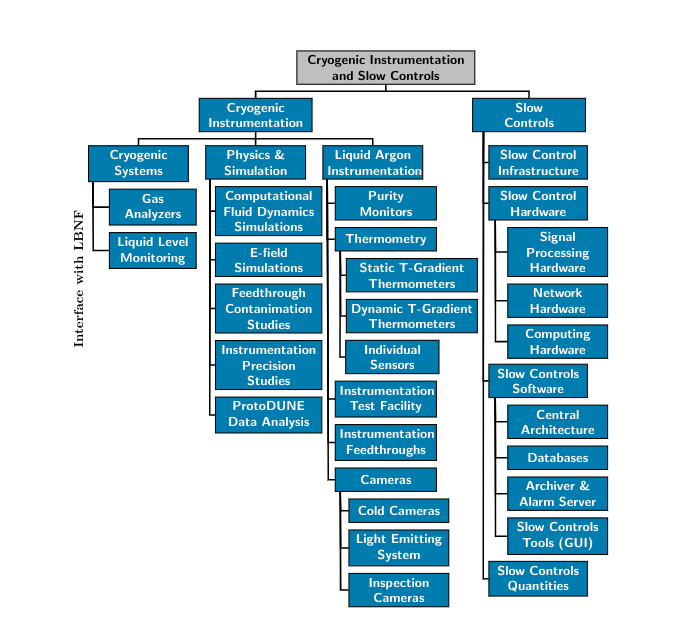
\includegraphics[width=0.6\textwidth]{CISC_scope-v3_TDR.png}
\end{dunefigure}

Two main branches can be distinguished: cryogenics instrumentation and slow controls. The former includes a set of instrumentation devices to monitor the quality and behavior of the \lar volume in the cryostat interior, ensuring the correct functioning of the full cryogenics system and the suitability of the \lar for good quality physics data. The second branch of \dword{cisc} is the slow controls (SC) system, in charge of monitoring and controlling most detector elements, such as power supplies, electronics, racks, instrumentation devices, calibration devices, etc. 

For all \lar instrumentation devices, \dword{pdsp} designs are
considered as the baseline, and requirements for most design
parameters are extrapolated from \dword{pdsp}. Hence the \dword{pdsp} data will be used to validate the instrumentation designs and to understand their performance.

\subsection{Components}
% \fixme{SG: Done. Editors, please check --- looks good [gahs]}

The devices included under cryogenics instrumentation are purity monitors,  different types of temperature monitors, and cameras with their associated light emitting system. Also included are components such as gas analyzers and \lar level monitors which are directly related to the external cryogenics system and thus have substantial interfaces with \dword{lbnf}. A test facility for the instrumentation devices is also included as part of the cryogenics instrumentation.

Cryogenics instrumentation also requires significant physics and
simulation work such as \efield simulations and cryogenics modeling
studies using \dfirst{cfd}. \efield simulations
are required to identify desirable locations for instrumentation
devices in the cryostat so that they are not in regions of high \efield and that their presence does not induce large field distortions. 
% AC. What do we mean by distortions here ?
% Alternative: ``that their designs do not induce high \efields and risk of dielectric breakdown. ``
\dshort{cfd} simulations are needed to understand the expected temperature, impurity and velocity flow distributions and guide the placement and distribution of instrumentation devices inside the cryostat.

The slow controls includes three main components: hardware, infrastructure, and software. The slow controls hardware and infrastructure consists of networking hardware, signal processing hardware, computing hardware, and relevant rack infrastructure. The slow controls software is needed for signal processing, alarms, archiving, and control room displays.

\subsection{Scope}
%\fixme{SG: Done. Editors, please check --- GAHS: added a few words, please check; SG: Checked, looks good!}

As described in the previous section, and shown schematically in Figure~\ref{fig:cisc-subsystem-chart}, the scope of the \dword{cisc} system spans a broad range of activities. In the case of cryogenics systems (gas analyzers and liquid level monitors), \dword{lbnf} provides the needed expertise and is responsible for the design, installation, and commissioning activities while the \dword{cisc} consortium provides the resources and supplements the labor as needed. In the case of \dword{lar} instrumentation devices (purity monitors, thermometers, cameras and light-emitting system; and their associated feedthroughs) and instrumentation test facility, CISC is responsible from design to commissioning in the \dwords{fd}.

For slow controls, \dword{cisc} provides software and infrastructure for controlling and monitoring of all detector elements that provide data on the health of the detector module or conditions important to the experiment, as well some related hardware. The scope of systems that slow controls includes is detailed below:

\textbf{Slow controls base software and databases:} provides the central tools needed to develop
control and monitoring for various detector systems and interfaces.
\begin{itemize}
\item Base input/output software,
\item Alarms; archiving; display panels; operator interface tools,
\item Slow controls system documentation and operations guidelines.
\end{itemize}
%
\textbf{Slow controls for external systems:} export data from systems external to the detector and provide status monitoring for operators and archiving.
\begin{itemize}
\item Beam status; cryogenics status; data acquisition (DAQ) status; facilities systems status,
\item For the systems above, import other interesting monitoring data as needed (e.g., pumps
data from cryogenics system, heaters data from facility systems, etc.),
\item Building controls; detector hall monitoring; ground impedance monitoring,
\item Interlock status bit monitoring (but not the actual interlock mechanism).
\end{itemize}
%
\textbf{Slow controls for detector hardware systems:} develop software interfaces for detector hardware devices
\begin{itemize}
\item Monitoring and control of all power supplies,
\item Full rack monitoring (rack fans, thermometers and rack protection system),
\item Instrumentation and calibration device monitoring (and control to the extent needed),
\item Power distribution units monitoring; computer hardware monitoring,
\item High voltage system monitoring through cold cameras,
\item Detector components inspection through warm cameras.
\end{itemize}
%
\textbf{Slow controls hardware:} \dword{cisc} will develop, install and commission any hardware related to rack monitoring and control. While most power supplies might only need a cable from the device
to an Ethernet switch, some power supplies might need special cables ({\em e.g.}, GPIB or RS232) for communication. The \dword{cisc} consortium will be responsible for providing such control cables.

In addition to the listed activities, \dword{cisc} also has activities that span outside the scope of the consortium and require interfacing with other groups. This is discussed in Sec.~\ref{sec:interfaces}.

\subsection{Requirements}
%\fixme{GAHS: text looks good; some numbers need to be replaced with latex commands from defs.tex or parameters.tex}

Some of the common design considerations for instrumentation devices include stability, reliability and longevity such that the devices can survive for a period of at least \dunelifetime. Since it is uncommon for any device to have such a long lifetime, provisions are made in the overall design to allow replacement of devices where possible. As for any other element inside the cryostat, the \efield  on the instrumentation devices is required to be less than \localefield, so that the risk of dielectric breakdown in \dword{lar} is minimized. Another important design parameter, which should be evaluated in \dword{pdsp}, is the maximum noise level induced by instrumentation devices on the readout electronics that can be tolerated to avoid confusing event reconstruction. Table~\ref{tab:fdgen-slow-cryo-requirements-1} and \ref{tab:fdgen-slow-cryo-requirements-2} show the full set of requirements for the different \dword{cisc} subsystems.
% \todo{SG: In table 1.2, there are "(???)" next to heat transfer. Needs to be fixed.  GAHS: fixed.}

Data from purity monitors and different types of thermometers will be used to validate the liquid argon fluid flow model and a number of requirements drive the design parameters for these systems to achieve the needed precision and granularity in their distribution across the cryostat. For example, the electron lifetime measurement precision is required to be 1.4\% in order to keep the bias on the charge readout in the \dword{tpc} to below 0.5\% at 3~ms lifetime. In the case of thermometers, the requirements are driven by the \dshort{cfd} simulations based on \dword{pdsp} design. The resolution and relative precision of temperature measurements
\footnote{The resolution is defined as the temperature RMS for individual measurements, and is driven by the electronics. The relative precision includes also the effect of reproducibility for successive inversions in LAr.}
is required to be less than 2~mK and 5~mK, respectively. The later is particularly important since gradients below 20~mK should be characterized.  
As will be described below, the laboratory calibration data and the recent analysis of thermometer instrumentation data from \dword{pdsp} showed that a 2.5~mK relative precision is achievable. 

The level meters are required to have a precision of 0.1\% over 14~m (14~mm) for measurement accuracy during filling. This precision is also sufficient for \dword{sp} to ensure the \dword{lar} level is above the ground planes. As shown in the table~\ref{tab:fdgen-slow-cryo-requirements-2}, multiple requirements drive the design of cold and warm cameras, and the associated light emitting system. It is important to ensure that none of the components of the camera systems contaminate the liquid argon or produce bubbles when the \dword{hv} is on as it increases the risk of \dword{hv} discharge. Both cold and warm cameras are required to provide a coverage of at least 80\% of the \dword{tpc} with a resolution of 1~cm and 2~mm on the \dword{tpc} for cold and warm cameras, respectively.
% CEL: my 'fixme' with details, removed. Wanted to hold 
% if needed later in the document. 

In the case of cryogenic test facility, a cryostat of 0.5 to about 3 cubic meter capacity is found to be reasonable as turn-around times are better for smaller cryostats, as well as filling costs. For gas analyzers, operating range forms an important requirement, details of which are shown in table~\ref{tab:fdgen-slow-cryo-requirements-1}.

For slow controls, the system will need to be designed to be robust enough to support a large number of monitored variables with a minimum of 50,000 variables and a broad range of monitoring and archiving rates. The system should also be able to interface with a large number of detector sub-systems to establish two-way communication for control and monitoring. 

% \fixme{Requirements table: replace ALARA with number or clear criterion, per reviewer comments. [gahs]; SG: I suggest using ENC < 1000 e$^{-}$ for minimum requirement and ALARA as goal. --- done [gahs]}

\begin{dunetable}
[Requirements for CISC subsystems]
{p{0.45\linewidth}p{0.25\linewidth}p{0.25\linewidth}}
{tab:fdgen-slow-cryo-requirements-1}
{List of requirements for the different CISC subsystems}   
Quantity/Parameter				                             & Minimum Requirement			                                        & Goal		                                              \\ \toprowrule                     
Noise from Instrumentation devices				             & <\elecnoisefe                                          & \dword{alara}		                                              \\ \colhline                     
Max. \efield near instrumentation devices				     & <\localefield			                                                & <15 kV/cm		                                          \\ \colhline                     
\textbf{Purity Monitors}	                                             &                                                                      &                                                         \\ \colhline                      
Precision in electron lifetime				                 & <1.4\% (<4\%)			                                            & < 1\%		                                              \\ \colhline                     
Range in electron lifetime				                     & 0 - 10 ms                   (0 - 30 ms)			                    & 0 - 10 ms                   (0 - 30 ms)		          \\ \colhline                         
Longevity				                                     & \dunelifetime			                                                    & > \dunelifetime		                                      \\ \colhline                     
Stability				                                     & Match precision requirement at all places/times			    & Match precision requirement at all places/times  \\ \colhline  	                   
Reliability				                                     & Daily Measurements			                                        & Measurements capable of being taken whenever needed	  \\ \colhline                         
\textbf{Thermometers}	                                             &                                                                      &                                                         \\ \colhline                      
Vertical density of sensors for T-gradient monitors			 & > 2 sensor/m			                                                & > 4 sensors/m		                                      \\ \colhline                 
2D horizontal density for top/bottom individual sensors		 &  1 sensor/5(10) m 			                                        &  1 sensor/3(5) m 		                                  \\ \colhline                     
Resolution of temperature measurements				         & < 2 mK			                                                    & <0.5 mK		                                          \\ \colhline                         
Precision: temperature reproducibility 				         & < 5 mK			                                                    & 2 mK		                                              \\ \colhline                     
Reliability				                                     & 80\% (in 18 months)			                                        & 50\% (during 20 years)		                              \\ \colhline                     
Longevity				                                     & > 18 months			                                                & > 20 years		                                      \\ \colhline                         
Stability 				                                     & Match precision requirement at all places/times 			    & 		                                                  \\ \colhline                 
Discrepancy between lab and in-situ                                                                                                   		                                          
calibrations for temperature sensors			             & < 5 mK			                                                    & < 3 mK		                                          \\ \colhline                           
Discrepancy between measured temperature                                                                                                                                                      
map and CFD simulations in ProtoDUNE-SP	                     & < 5 mK			                                                    & < 5 mK		                                          \\ \colhline                             
\textbf{Gas Analyzers}	                                             &                                                                      &  \\ \colhline            
Operating Range O2				                             & 0.2 (air) to 0.1 ppt			                                        & Air (0.2) to 0.1 ppt		                                             \\ \colhline    
Operating Range H2O				                             & Nominally Air to sub ppb levels, depending on species of contaminant	& Air to sub ppb levels, depending on species of contaminant	          \\ \colhline           
Operating Range N2				                             & Nominally Air to sub ppb levels, depending on species of contaminant	& Air to sub ppm.		                                              \\ \colhline             
Precision: 1 sigma at zero				                     & depends on the range of the gas analyzer			                    & depends on the range of the gas analyzer		                      \\ \colhline     
Detection limit: 3 sigma				                     & Different Gas analyzer modules are needed to cover the entire range	& Different Gas analyzer modules are needed to cover the entire range \\ \colhline           
Stability 				                                     & <\% of full scale range.			                                    & <\% of full scale range.		                                      \\ \colhline         
Longevity				                                     & >10 years			                                                & 10 years		                                                      \\   
\end{dunetable}


\begin{dunetable}
[Requirements for CISC subsystems]
{p{0.45\linewidth}p{0.25\linewidth}p{0.25\linewidth}}
{tab:fdgen-slow-cryo-requirements-2}
{List of requirements for the different CISC subsystems}   
Quantity/Parameter				                             & Minimum Requirement			                                        & Goal		                                              \\ \toprowrule   
\textbf{Level Meters}	                                             &                                                                      &                                                                     \\ \colhline            
Precision (LBNF side)				                         & 0.1\% over 14 m (14 mm)			                                    & 0.1\% over 14 m (14 mm)		                                      \\ \colhline           
Precision (additional level meters, DUNE side)				 & 20 mm			                                                    &  20 mm		                                                      \\ \colhline         
Longevity				                                     & 20 years			                                                    & > 20 years		                                                  \\ \colhline     
\textbf{Cold cameras}	                                             &                                                                      &                                                                     \\ \colhline        
Coverage				                                     & 80\% of the exterior of HV surfaces			                        & 100\% 	                                                          \\ \colhline         
Frames per second				                             & yet to be defined			                                        & yet to be defined		                                              \\ \colhline             
Resolution 				                                     & 1 cm on the TPC			                                            & yet to be defined		                                              \\ \colhline           
Duty cycle				                                     & yet to be defined			                                        & yet to be defined		                                              \\ \colhline         
longevity				                                     & > 18 months			                                                & > 20 years		                                                  \\ 
\textbf{Inspection cameras}	                                         &                                                                      &                                                                     \\ \colhline        
Coverage				                                     & 80\% of the TPC			                                            & yet to be defined		                                              \\ \colhline         
Frames per second				                             & yet to be defined			                                        & yet to be defined		                                              \\ \colhline             
Resolution 				                                     & 2 mm on the TPC			                                            & yet to be defined		                                              \\ \colhline           
heat transfer				                             & no generation of bubbles			                                & 	no generation of bubbles		                                                              \\ \colhline         
longevity				                                     & > 18 months			                                                & > 20 years		                                                  \\ \colhline         
\textbf{Light emitting system}	                                     &                                                                      &                                                                     \\ \colhline        
radiant flux 				                                 & > 10 mW/sr			                                        & 
100 mW/sr \\ \colhline         
power				                                         & < 125 mW/LED			                                        & \dword{alara}		                                              \\ \colhline           
wavelength				                                     & red/green			                                            & IR/white		                                              \\ \colhline         
longevity				                                     & > 18 months (for cold cameras) 			                            & > 20 years		                                              \\ \colhline         
\textbf{Cryogenics Instrumentation Tests Facility}	                 &                                                                      &                                                                     \\ \colhline            
Dimensions				                                     & 0.5-~3  cubic meters 			                                    & 0.5-3 cubic meters		                                          \\ \colhline             
Temperature stability				                         & +-1K			                                                        & +- 1K		                                                          \\ \colhline                                       
Turn-Around time				                             & ~9 days			                                                    & 9 days 		                                                      \\ \colhline                                       
LAr purity				                                     & O2 and H2O low enough  to measure drifting                            		                                                      
                                                               electrons of devices under test, ~0.5ms.                                                                        
                                                               N2 levels at the ppm level for scintillation light tests. 	        &  >1.0 ms                                                            \\ \colhline
\textbf{Slow Controls}		                                         &                                                                      &                                                                     \\ \colhline
Alarm rate				                                     & <150/day			                                                    &  < 50/day                                                           \\ \colhline
Total No. of variables				                         & 150,000			                                                    &  150,000 - 200,000                                                   \\ \colhline
Server rack space				                             & 2 racks			                                                    &  3 racks                                                            \\ \colhline
Archiving rate 				                                 & 0.02 Hz			                                                    &  Broad range 1 Hz  to 1 per few min.                                \\ \colhline
Near Detector Status				                         & Beam Conditions and Detector Status	                                &  Full Beam and Detector Status                                      \\          
\end{dunetable}                                  

%%%%%%%%
\section{Fluid Dynamics Simulation}
The overall goal of the fluid dynamics simulations for the DUNE detectors is to better understand and predict the fluid (in either a liquid and vapor state) motions and its implication on the performance of the detectors. The fluid flow behavior can be determined through simulation of \dword{lar} flow within the detector using Siemens Star-CCM$+$\footnote{https://mdx.plm.automation.siemens.com/star-ccm-plus}, a commercially available computational fluid dynamics (CFD) code. Such a model must include proper definition of the fluid characteristics, solid bodies and fluid-solid interfaces, and a means for measuring contamination, while still maintaining reasonable computation times. In addition, these fluid dynamics simulations are compared with available experimental data to assess the simulations' accuracy and credibility. 

Although simulation of the detector module presents challenges, there exist acceptable simplifications for accurately representing the fluid, the interfacing solid bodies, and variations of contaminant concentrations. Because of the magnitude of thermal variation within the cryostat, modeling of the \dword{lar} is simplified through use of constant thermophysical properties, calculation of buoyant force through use of the Boussinesq Model (using a constant density for the fluid with application of a temperature dependent buoyant force), and a standard shear stress transport turbulence model. Solid bodies that contact the \dword{lar} include the cryostat wall, the cathode planes, the anode planes, the \dword{gp}, and the \dword{fc}. As in previous \dword{cfd} models of the \dword{dune} 35-ton prototype and \dword{protodune} by South Dakota State University (SDSU) \cite{docdb-5915}, the \dword{fc} planes, anode planes, and \dword{gp} can be represented by porous bodies. Since impurity concentration and electron lifetime do not impact the fluid flow, these variables can be simulated as passive scalars, as is commonly done for smoke releases \cite{cfd-1} 
in air or dyes released in liquids.

Proper placement of purity monitors, thermometers, and liquid level monitors within the detector module requires knowledge of how \dword{lar} flows within the cryostat in terms of its fluid dynamics, heat and mass transfer, and distribution of impurity concentrations. Fluid motion within the cryostat is driven primarily by small changes in density caused by thermal gradients within the fluid, although pump flow rates and inlet and outlet locations also contribute. Heat sources include exterior heat from the surroundings, interior heat from the electronics, and heat flow through the pump inlet. In principle, purity monitors can be placed throughout the cryostat to determine if the argon is pure enough for experimentation. However, there are areas inside the cryostat that are off limits for such monitors. In order to determine the purity of the argon in regions where experimental data is unavailable, \dword{cfd} simulations can be used to better understand and quantify impurity levels.

Discrepancies between real data and simulations may have potential impacts on detector performance, as simulation results contribute to decisions about where to locate sensors and monitors, as well as definitions of various calibration quantities. However, methods of mitigating such risks include well established convergence criteria, sensitivity studies, and comparison to results of previous CFD simulation work by SDSU and Fermilab. Additionally, the simulation will be improved with input from temperature measurements and validation tests from \dword{protodune}.

%%%%% Must find better pictures. Just use this for now
\begin{dunefigure}[\dshort{cfd} example]{fig:cfd-example}
  {Distribution of temperature on a plane intersecting an inlet (right) and halfway between an inlet and an outlet (left), as predicted by SDSU \dshort{cfd} simulations (from~\cite{docdb-5915}). (See Fig.~\ref{fig:cfd-example-geometry} for geometry.)}
  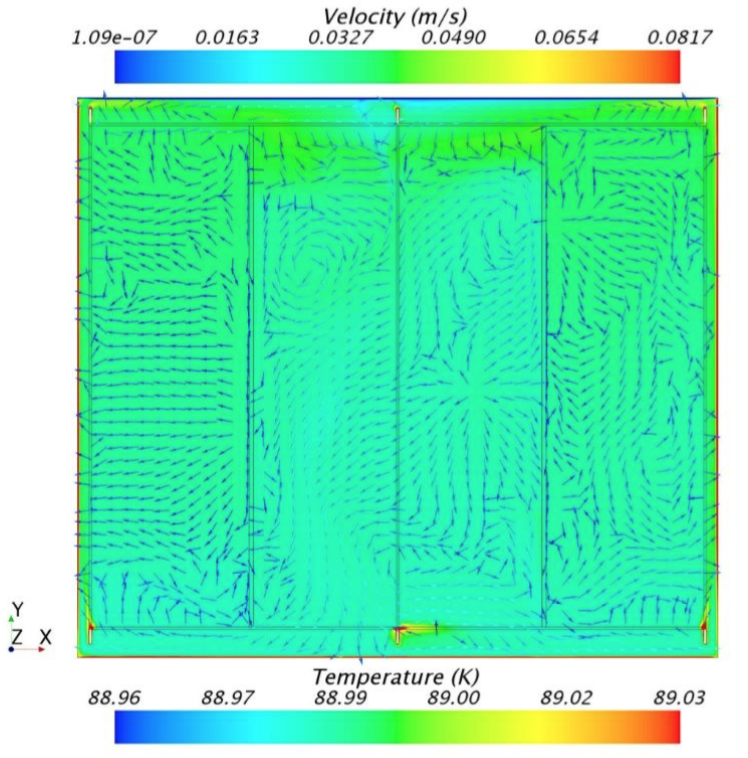
\includegraphics[height=0.4\textwidth]{cisc_cfd_outlet_z0.png}
  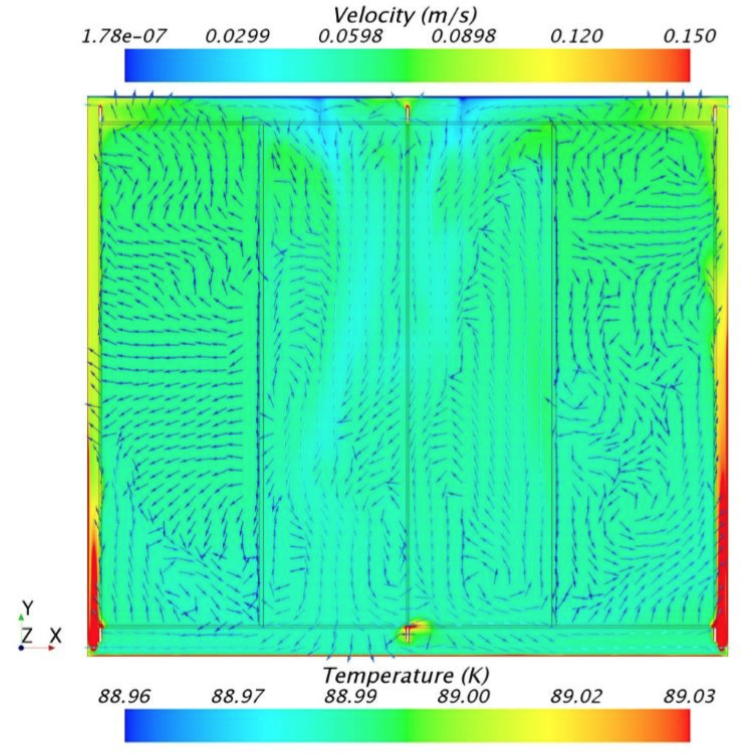
\includegraphics[height=0.4\textwidth]{cisc_cfd_inlet_z52.png}
\end{dunefigure}

Fig.~\ref{fig:cfd-example} shows an example of the temperature
distribution on a plane intersecting a \dword{lar} inlet and at a
plane halfway between an inlet and an outlet; 
the geometry used for
this simulation is shown in Fig.~\ref{fig:cfd-example-geometry}. Note the plume of higher temperature \dword{lar} between the walls and
the outer APA on the inlet plane. The current locations of instrumentation in
the cryostat as shown in Fig.~\ref{fig:cisc-tsensor-map} were determined using the temperature and impurity distributions from these previous simulations.

\begin{dunefigure}[\dword{cisc} geometry layout]{fig:cfd-example-geometry}
  {Layout of the \dword{tpc} within the cryostat (top) and positions of \dword{lar} inlets and outlets (bottom) as modeled in the SDSU \dword{cfd} simulations~\cite{docdb-5915}. The Y axis is vertical and the X axis is parallel to the \dword{tpc} drift direction. Inlets are shown in green and outlets are shown in red.}
  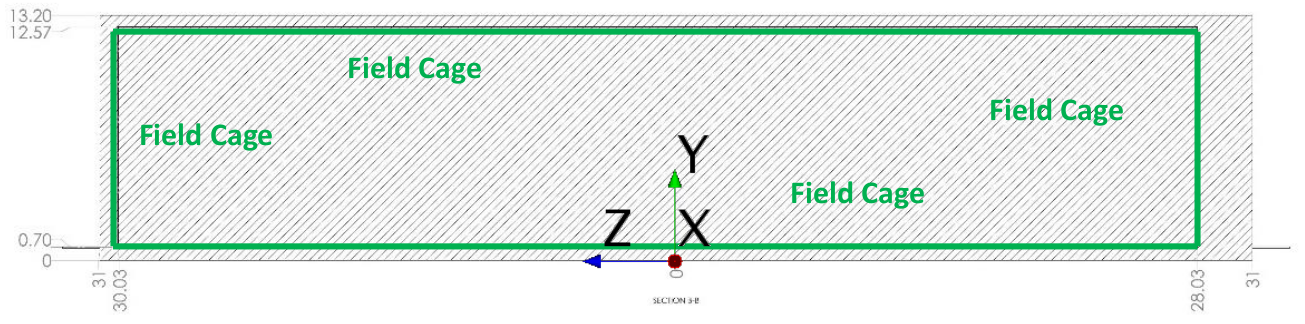
\includegraphics[width=0.7\textwidth]{cisc_cfd_cryostat-layout.png}
  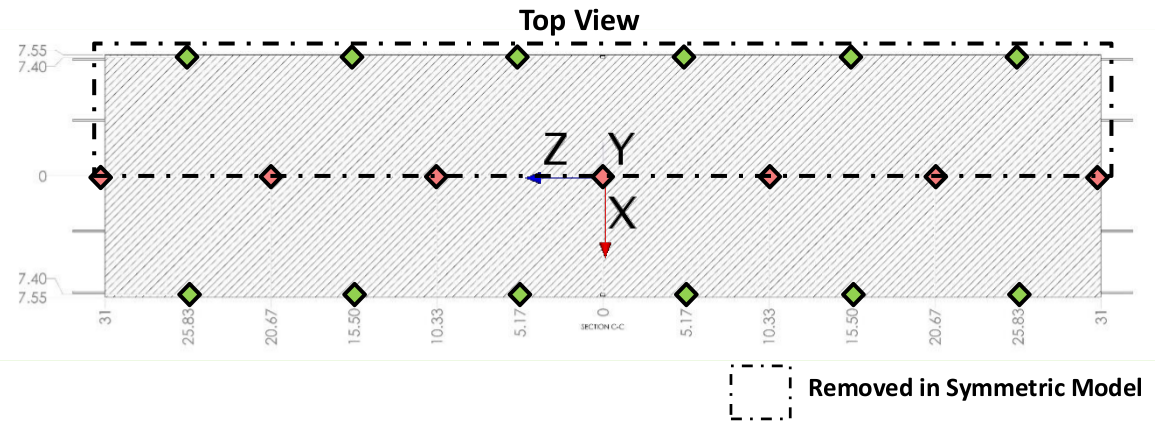
\includegraphics[width=0.7\textwidth]{cisc_cfd_inlet-outlet-layout.png}
\end{dunefigure}

The strategy for the future \dword{cfd} simulation effort is to understand the performance of ProtoDUNE-SP cryogenics system and model the far detectors to derive requirements for instrumentation devices. The following is a prioritized set of studies planned (some currently underway) to help drive the requirements for other systems:
\begin{itemize}
\item Review the \dword{dune} \dword{fd} cryogenics system design and verify the current implementation in simulation; this is important to ensure that the model represents what will be built.
\item 
Model the ProtoDUNE-SP liquid and gas regions with the same precision as the \dword{fd}. Presently only the liquid model exists. The liquid model is needed to interpret the thermometer data, and the gas model is needed to understand how to place thermometers in the ullage and verify the design of the gaseous argon purge system.
% \item Perform a \dword{cfd} study to determine the feasibility of a wier for DP; this helps to determine if it can be used to clean the \dword{lar} surface before the extraction grid is submerged in the DP module.
\item Verify the SP \dword{cfd} model for the \dword{fd} SP module in simulation performed by LBNF; this defines the requirements for instrumentation devices (e.g., thermometry).
% \item Model the ProtoDUNE-DP liquid and gas regions with the same precision as the \dword{fd}.
\end{itemize}

\begin{dunetable}
[CFD parameters for \dword{protodune}]
{p{0.25\textwidth}p{0.15\textwidth}p{0.5\textwidth}}
{tab:fdgen-cisc-CFDparam}
{CFD input parameters for \dword{protodune}}   


Parameter  &	Value &	Comments \\ \toprowrule
Cryostat height
&
7.878 m
&
Measured with laser (1 cm error approx.)
\\ \toprowrule	
LAr surface height
&
7.406 m
&
Measured by capacitive level meter ($<1$ cm error)
\\ \toprowrule	
Ullage pressure		
&
1.045 bar
&
Measured by pressure gauges
\\ \toprowrule
LAr surface temperature
&
87.596 K
&
computed using ullage pressure and \linebreak
https://lar.bnl.gov/properties/basic.html\#phase
\\ \toprowrule
LAr inlet temperature
&
outlet + 0.2 K
&
Estimated
\\ \toprowrule
LAr flow rate per pipe
&
0.4170025 kg/s
&
\\ \toprowrule		
Heat flux 
&
5.76 $W/m^2$		
&
This is the Heat flux from all four walls as well as the ground
\\ \toprowrule
Vapor being drawn from the chimneys
&
5-7 gr/sec
&
among all chimneys
\\
\end{dunetable}

\subsection{Validation in ProtoDUNE}

The data we can collect at ProtoDUNE-SP to validate \dword{cfd} is already set by the installed instrumentation:
\begin{itemize}
\item Static and Dynamic T-gradient thermometers
\item Individual temperature sensors placed in the return \dword{lar} inlets
\item two 2D grids of individual temperature sensors, located below the bottom ground planes and above the top ground planes
\item a string of three purity monitors vertically spaced from near the bottom of the cryostat to just below the \dword{lar} surface
\item H$_{2}$O, N$_{2}$, and O$_{2}$ Gas analyzers
\item \dword{lar} level monitors
\item standard cryogenic sensors such as pressure transducers, various individual temperature sensors placed around
the cryostat on the membrane walls, and recirculation flow rates transducers
\end{itemize}

These devices are up and running and have already been producing data which is logged through slow controls and available for offline analysis.

The temperature profiles of the ProtoDUNE-SP simulation are currently being compared with experimental temperature probe data. Although this work is ongoing preliminary results exist. Fig.~\ref{fig:cisc-cfd-valid} shows the fluid temperature measured by the temperature probe and how it compares with the current ProtoDUNE-SP \dword{cfd} model with parameter shown in Table \ref{tab:fdgen-cisc-CFDparam}.\todo{Confirm this table is referenced correctly as input parameters to the iteration procedure for comparison with temperature probes.} 
The validation procedure consists on an iterative process in which several versions of the \dword{cfd} simulations have been produced with different input parameters to converge on a reasonable agreement. 

\begin{dunefigure}[Comparison between ProtoDUNE-SP temperature data and CFD simulations]{fig:cisc-cfd-valid}
  {Comparison between ProtoDUNE-SP temperature data and CFD simulations.}
  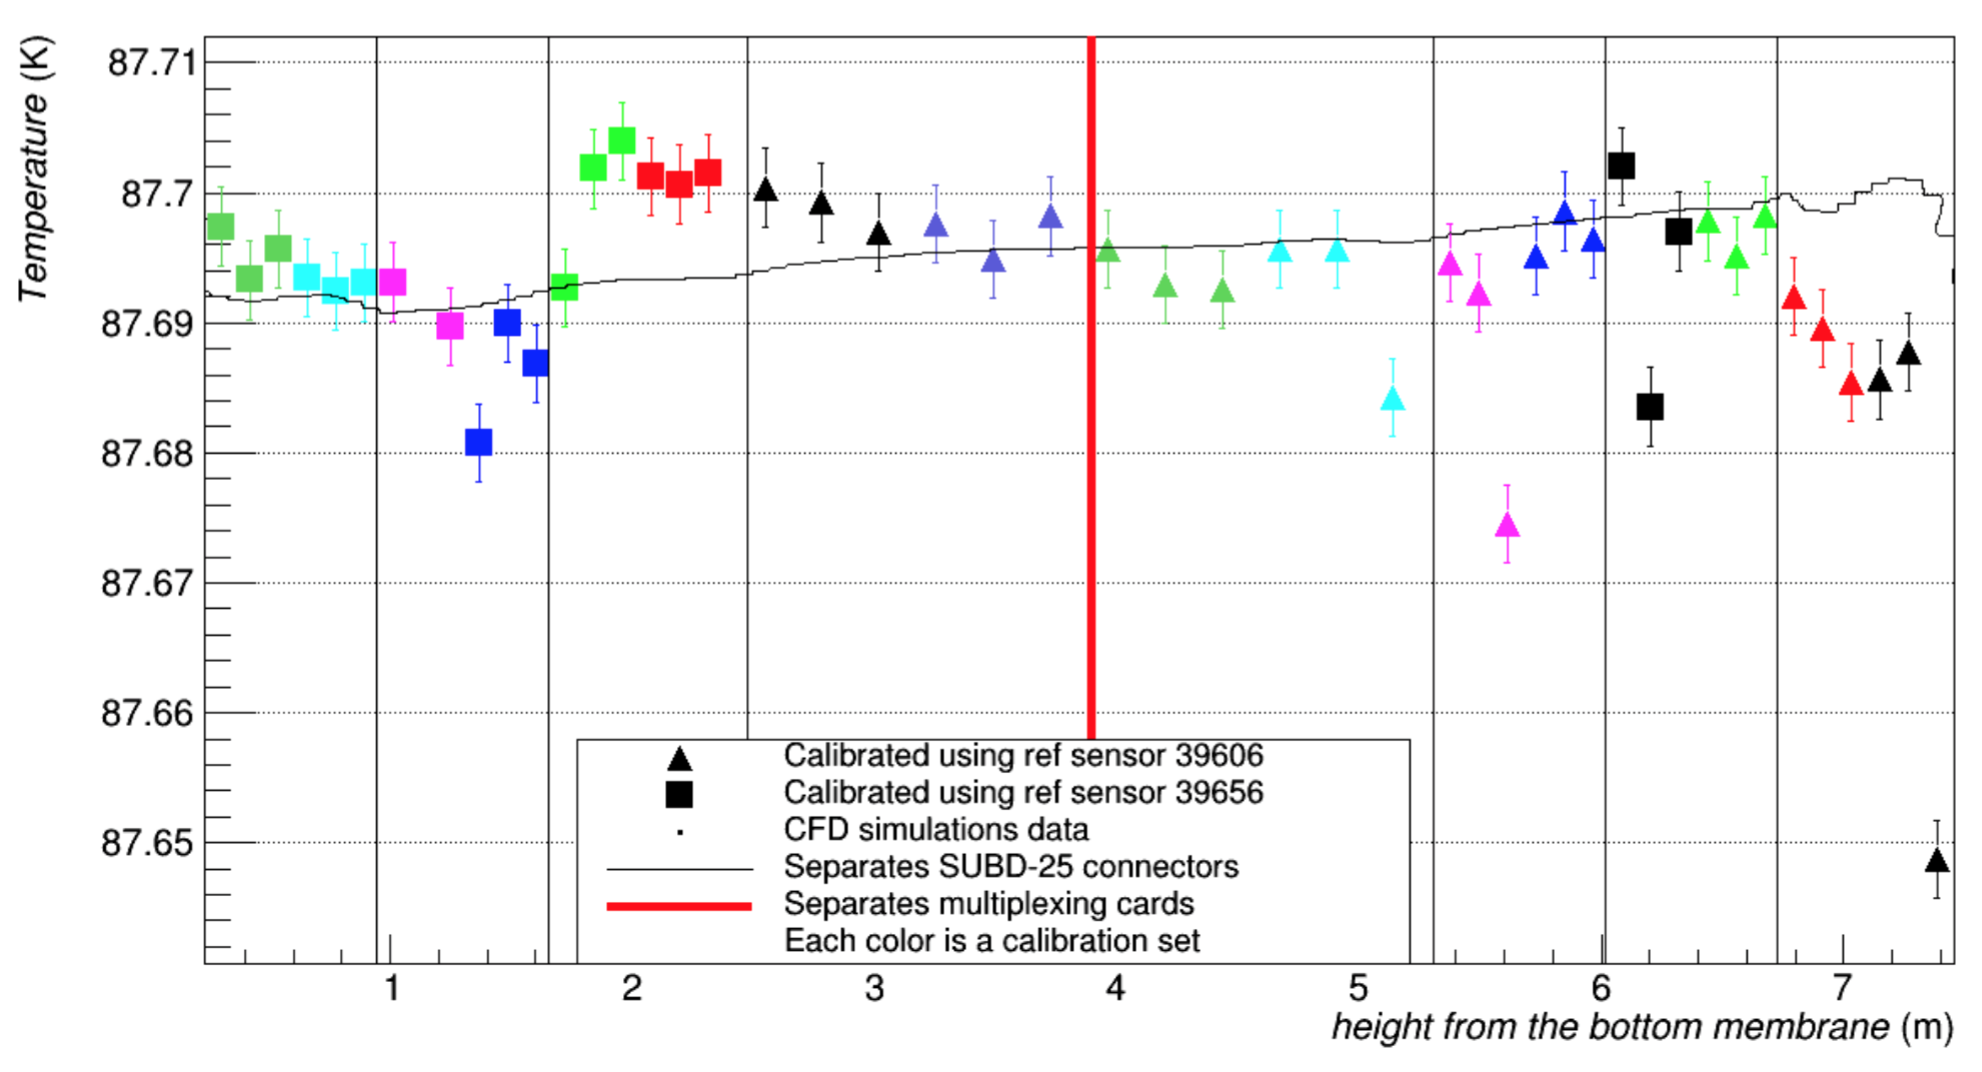
\includegraphics[width=0.6\textwidth]{cisc_CFD_valid_v0.png}
\end{dunefigure}

After further refinement of the \dword{cfd} models, additional data from purity monitors will be compared with the results to make sure that the simulations can accurately map impurity levels in the detector. Streamlines\footnote{In fluid mechanics, a streamline is a line that is everywhere tangent to the local velocity vector. For steady flows, a streamline also represents the path that a single particle of the fluid will take from inlet to exit.} from the current ProtoDUNE-SP simulation (Fig.~\ref{fig:cisc-cfd-larflow-inlets}) show the flow paths from the four inlets to the outlet of the cryostat.

\begin{dunefigure}[lar flow inlets]{fig:cisc-cfd-larflow-inlets}
  {Streamlines for liquid argon flow inside of the ProtoDUNE-SP detector.}
  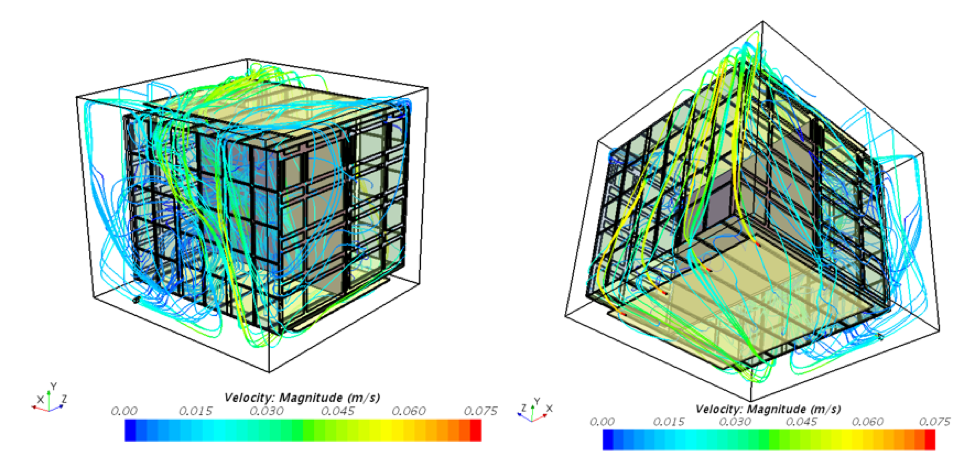
\includegraphics[width=0.8\textwidth]{cisc_cfd_larflow-inlets.png}
\end{dunefigure}

In the future, additional dedicated tests are also planned towards \dword{cfd} validation as provoking changes to the cryostat environment and measuring the instrumentation response may assist in establishing the validation of the \dword{cfd} model. Seeing that the \dword{cfd} predicts a reasonable response for more than one set of initial conditions is reassuring. For these additional tests, it is reasonable to wait until the beam run is finished, since they could have undesirable impacts on the cryostat environment. Some of the additional tests that could be done include pump/recirculation manipulations such as pump on/off, pumping speed change and bypassing filtration. Additionally, one can also induce changes in the pressure by setting the cryostat pressure set point to a higher (or lower) value\footnote{One may want the HV to be ramped down for this exercise, since dropping the pressure too fast might provoke boiling of the LAr near the
surface.} for a specified time and the instrumentation monitored. Any change in pressure has the potential to change the temperature everywhere in the cryostat. Studying the rate of this change, as
detected in the various vertical heights of the cryostat might provide interesting constraints on the \dword{cfd} model. 

%\fixme{The plan is to PRODUCE A NEW MAP WITH THE HAWAII DATA INCLUDED AND THE NEW CFD SIMULATION, BY THE END OF DECEMBER. Text will be updated accordingly to discuss new results.}

%%%%%%%%
\section{Cryogenic Instrumentation}
\label{sec:fdgen-cryo-instr}
Instrumentation inside the cryostat must ensure that the condition of the \dword{lar} is adequate for operation of the \dshort{tpc}.
This instrumentation includes devices to monitor the impurity level of the argon, e.g., the purity monitors, which provide high-precision electron lifetime measurements,
and gas analyzers to ensure that the levels of atmospheric contamination drop below certain limits during the cryostat purging, cooling and filling.
The cryogenics system operation is monitored by temperature sensors deployed in vertical arrays and at the top and bottom of the detector, providing a 
detailed \threed temperature map that can help to predict the \dword{lar} purity across the entire cryostat. The cryogenics instrumentation also includes \lar level monitors and
a system of internal cameras to help in locating sparks in the cryostat and for overall monitoring of the cryostat interior. 

%Reference to CFD (lo que esta escrito no vale, es un primer intento copiando la introduccion de la seccion CFD)
As mentioned in previous section, fluid motion within the cryostat needs to be simulated using a \dfirst{cfd} code.
The proper placement of purity monitors, thermometers, and liquid level monitors within the \dword{detmodule} requires knowledge of how \dword{lar} behaves within the cryostat in terms of its fluid dynamics, heat and mass transfer, and distribution of impurity concentrations. Besides that, the coherent analysis of the instrumentation data needs the results of such simulations.

%Something on ProtoDUNE Validation 
The performance of all cryogenic instrumentation for DUNE-FD is being tested in ProtoDUNE-SP, validating the baseline design for DUNE-FD.

%%%%%%%%%%%%%%%%%%%%%%%%%%%%%%%%%%%%%%%%%%%%%%%%%%%%%%
%%%%%%%%%%%%%%%%%  PURITY MONITORS %%%%%%%%%%%%%%%%%%%

%%%%%%%%%%%%%%%%%%%%%%%%%%%%%%%%%%%

\subsection{Purity Monitors}
\label{sec:fdgen-slow-cryo-purity-mon}

%Laura, Jianming
A fundamental requirement of a \dword{lar} \dshort{tpc} is that ionization electrons drift over long distances in \dword{lar}. Part of the charge is inevitably lost due to the presence of electronegative impurities in the liquid. To keep such loss to a minimum, purifying the \dword{lar} during operation is essential, as is the monitoring of impurities.




A purity monitor is a small ionization chamber that can be used to independently  infer the effective free electron lifetime in the \lartpc.  The operational principle of the purity monitor consists of generating a known electron current via illumination of a cathode with UV light, followed by collecting at an anode the current that survives after drifting a known distance.  The  attenuation of the current can be related to the electron lifetime.
The electron loss can be parameterized as
%
\(N(t) = N(0)e^{-t/\tau},\)
%
where $N(0)$ is the number of electrons generated by ionization, $N(t)$ is the number of electrons after drift time $t$, and $\tau$ is the electron lifetime. 

For the \dword{spmod}, the drift distance is \spmaxdrift and the \efield is \SI{500}{\volt\per\centi\meter}. Given the drift velocity at this field of approximately \SI{1.5}{\milli\meter\per\micro\second}, the time to go from cathode to anode is around \SI{\sim2.4}{\milli\second} \cite{Walkowiak:2000wf}.
The \dword{lar} \dshort{tpc} signal attenuation, \([N(0)-N(t)]/N(0)\), is to be kept less than \SI{20}{\percent} over the entire drift distance \cite{fdtf-final-report}. The corresponding electron lifetime is $2.4/[-\ln(0.8)] \simeq \SI{11}{ms}$.
% (The corresponding \dword{lar} O2 purity requirement is about \SI{30}{ppt}.)

Residual gas analyzers are an obvious choice when analyzing argon gas and can be exploited for the monitoring of the gas in the ullage of the tank. Unfortunately, commercially available and suitable mass spectrometers have a detection limit of \num{\sim10}\dword{ppb}, whereas DUNE requires a sensitivity down to the \dword{ppt} level. Instead, specially constructed purity monitors measure \lar purity in all the phases of operations, and enable the position-dependent purity measurements necessary to achieve DUNE's physics goal. 
%Purity monitors also have the potential to be developed as a calibration tool that provides high precision and real-time electron lifetime measurements for wire-by-wire detector calibration.

Purity monitors also serve to mitigate \lar contamination risk.  The large scale of the \dwords{detmodule} increases the risk of failing to notice a sudden unexpected infusion of contaminated \lar being injected back into the cryostat.   
If this condition were to persist, it could cause irreversible contamination to the \dword{lar} and terminate useful data taking.  Strategically placed purity monitors mitigate this risk, which has been demonstrated by the purity monitors installed in the \dword{pdsp} detector.

Purity monitors are placed inside the cryostat, but outside of the detector \dshort{tpc}, as well as outside the cryostat within the recirculation system before and after filtration. 
Continuous monitoring of  the \dword{lar} supply lines to the \dword{detmodule} provides a strong line of defense against contaminated \lar. Gas analyzers (described in Section~\ref{sec:fdgen-slow-cryo-gas-anlyz}) provide a first line of defense against contaminated gas.  Purity monitors inside the \dword{detmodule} provide the critical defense against liquid argon contamination caused by pump and filter problems, as well as all sources of contamination in the \lar volume and contamination from recirculated \lar. 

Furthermore, multiple purity monitors measuring lifetime with high precision at carefully chosen points can provide key inputs to \dshort{cfd} models of the detector, such as vertical gradients in impurity concentrations.

Purity monitors have been deployed in previous LArTPC experiments such as ICARUS, \microboone, and \dword{35t}. During the first run of the \dword{35t}, two out of four purity monitors stopped working during the cooldown, and a third was intermittent. It was later found out that this was due to poor electrical contacts of the resistor chain on the purity monitor. A new design was then implemented and successfully tested in the second run. 


The \dword{pdsp} and \dword{pddp} employ purity monitoring systems that consist of several purity monitors to measure electron lifetime at different heights. The assembly of the ProtoDUNE-SP purity monitors is shown in Figure~\ref{fig-pdsp-prmassembly}. Improvements in the design were made to ensure the electric connectivity and to improve signals. \dword{pdsp} utilizes a string of purity monitors connected with stainless steel tubes which protect the optic fibers. The purity monitor system at \dword{pdsp} measured electron lifetime on a hours base during the commissioning and on a daily base during the beam test. During the commissioning and test beam running, the purity monitor system at \dword{pdsp} has solely alerted the experiment to serious problems two times. The first time was the filter saturation and the second time was the fact that the recirculation pump had stopped. Those alerts are crucial to the success of the test beam running of the \dword{pdsp} project, as they prevented the situations which otherwise would have continued unnoticed for some time, with severe consequences to the ability to take any beam data.

\begin{dunefigure}[The ProtoDUNE-SP purity monitoring system]{fig-pdsp-prmassembly}
  {The ProtoDUNE-SP purity monitoring system}
  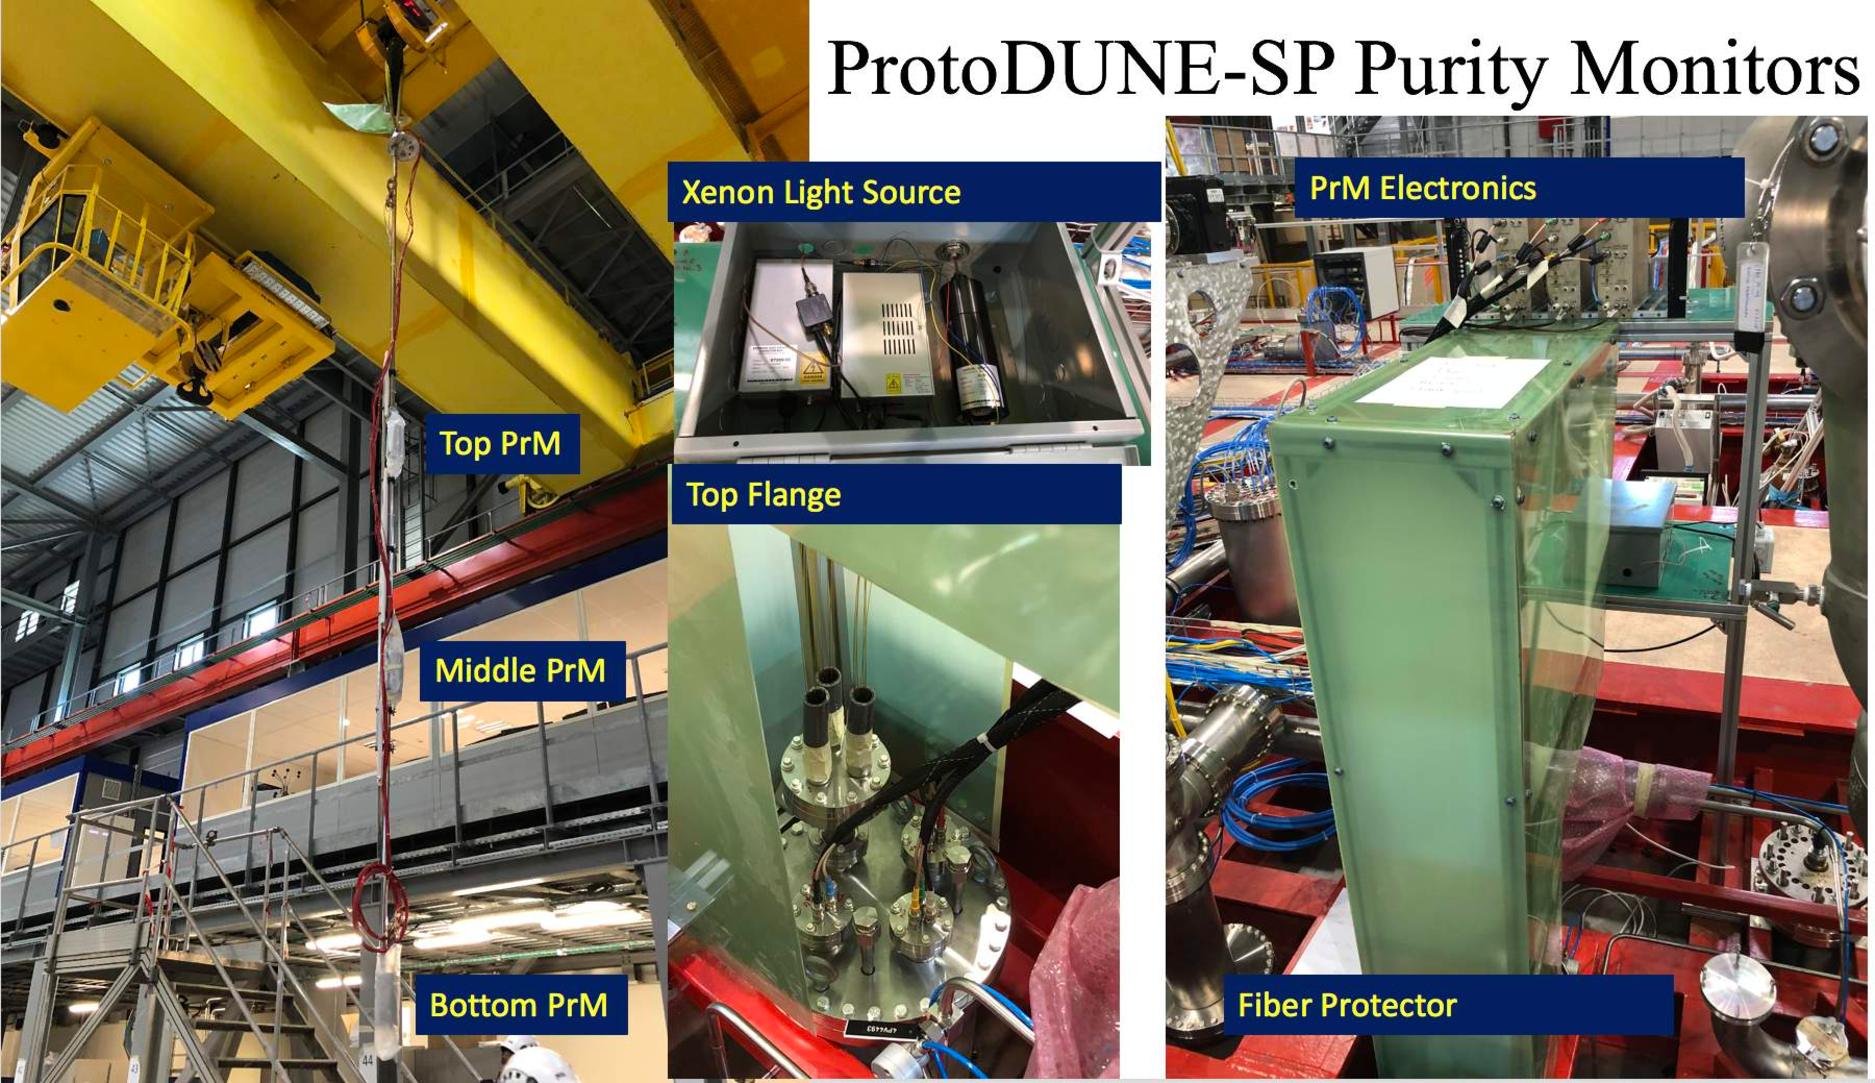
\includegraphics[width=0.9\textwidth]{PrMon_pdsp-PrMAssembly.pdf}
\end{dunefigure}



The \dword{pdsp}  purity monitors were operated with different high voltages to make electron drift time ranging from 150 $\mu$s to 3 ms. This allows the \dword{pdsp} purity monitors measuring electron lifetime from 35 $\mu$s to about 10 ms with high precision. In other words, the purity monitors are capable of measuring lifetimes over a dynamic range above 300. This high precision electron lifetime measurement is also valuable to the lifetime calibration for  \dword{pdsp}. Particularly, because the purity monitors have much small drifter volumes compared with the \dshort{tpc}, they are less affected by the space charge caused by the cosmic rays. 

  A similar purity monitoring system design and operation plan are exploited in the DUNE \dword{fd}, with modifications made to accommodate the instrumentation port placement relative to the purity monitor system and the requirements and constraints coming from the different geometric relations between the \dshort{tpc} and cryostat.




%%%%%%%%%%%%%%%%%%%%%%%%%%%%%%%%%%%%%%%%%%
%\subsubsection{Physics and Simulation}
% Andrew, Jianming





The \dword{pdsp} at CERN was instrumented with three purity monitors. The data taken with them from the commissioning of \dword{pdsp} in September, 2018 to the middle of test beam running, November, 2018, are shown in Figure~\ref{fig-pdsp-prm}. 

\begin{dunefigure}[The measured electron lifetimes in the four purity monitors as a function of time at ProtoDUNE-SP prototype]{fig-pdsp-prm}
  {The measured electron lifetimes in the four purity monitors as a function of time at ProtoDUNE-SP prototype.}
  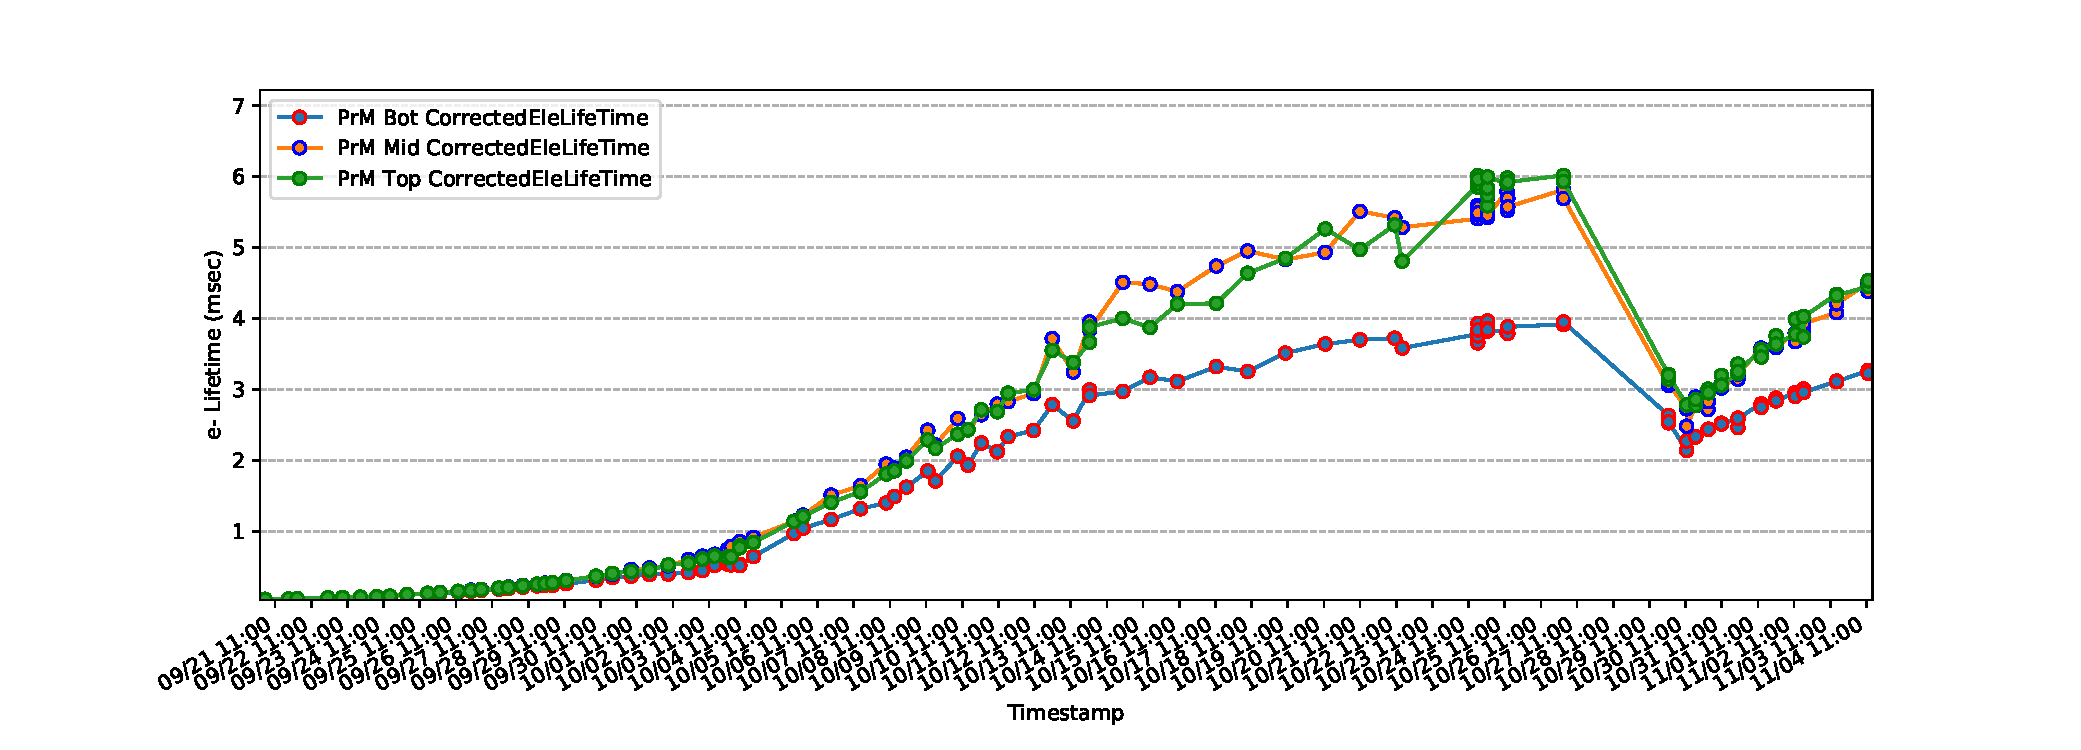
\includegraphics[width=0.9\textwidth]{PrMon_pdsp-PrM.pdf}
\end{dunefigure}




%%%%%%%%%%%%%%%%%%%%%%%%%%%%%%%%%%%%%%%%%
\subsubsection{Purity Monitor Design}
%Laura, Jianming
%WIP IF YOU HAVE MIP PARTICLES LIKE MUONS... NOT TRUE WHEN YOU ARE UNDERGROUND. ALSO, WE HAVE SEEN IN THE 311 THAT MUONS DO NOT DEPOSIT THE EXACT SAME AMOUNT OF ENERGY ACROSS THE TRACK 
%While the \dword{lar} \dshort{tpc} itself can measure the purity of the liquid argon based on the drift electron lifetime, this can only be done once a certain level of purity has been achieved, and until then it may be unclear what the level of purity is and if conditions in the detector are becoming better or worse. 

The basic design of a purity monitor is based on those used by the ICARUS experiment (Figure~\ref{fig:prm})\cite{Adamowski:2014daa}. It is a double-gridded ion chamber immersed in the \lar volume.   The purity monitor consists of four parallel, circular electrodes: a disk holding a photocathode, two grid rings (anode and cathode), and an anode disk. The cathode grid is held at ground potential. The cathode, anode grid, and anode are electrically accessible via modified vacuum grade high-voltage \fdth{}s and separate bias voltages held at each one.  
The anode grid and the field shaping rings are connected to the cathode grid by an internal chain of \SI{50}{\mega\ohm} resistors to ensure the uniformity of the \efield{}s in the drift regions. A stainless mesh cylinder is used as a Faraday cage to isolate the purity monitor from external electrostatic backgrounds. 

The purity monitor measures the electron drift lifetime between its anode and cathode. The electrons are generated by the purity monitor's UV-illuminated gold photocathode via the photoelectric effect. As the electron lifetime in \lar is inversely proportional to the electronegative impurity concentration, the fraction of electrons generated at the cathode that arrive at the anode ($Q_A/Q_C$) after the electron drift time $t$ gives a measure of the electron lifetime $\tau$:
%
\( Q_A/Q_C \sim e^{-t/\tau}.\)



\begin{dunefigure}[Schematic diagram of the basic purity monitor design]{fig:prm}
  {Schematic diagram of the basic purity monitor design \cite{Adamowski:2014daa}.}
  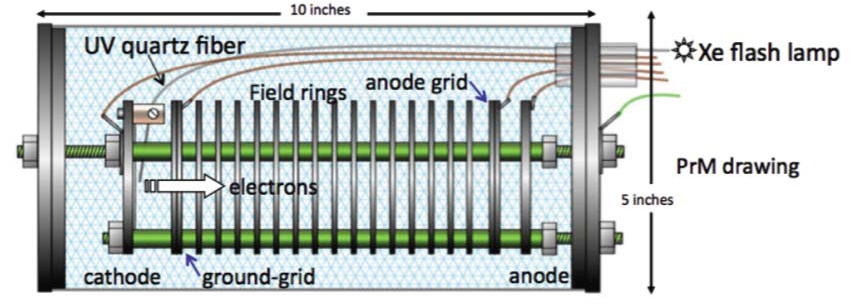
\includegraphics[width=0.9\textwidth]{PrMon_prm.pdf}
\end{dunefigure}


%
%Complete formula would be: Q_A/Q_C = \frac{T_1 \sinh(t_3/2\tau)}{t_3 \sinh(t_1/2\tau)} \exp \left(-\frac{t_2+\frac{t_1+t_3}{2}}{\tau} \right), where$t_1$ is the time it takes the electrons to go from cathode to cathode grid, $t_2$ to go from cathode grid to anode grid, and $t_3$ to go from grid anode to anode. 

It is clear from this formula that the purity monitor reaches its sensitivity limit once the electron lifetime becomes much larger than the drift time $t$. For $\tau >> t$ the anode to cathode charge ratio becomes $\sim\,1$. But, as the drift time is inversely proportional to the \efield, by lowering the drift field one can in principle measure any lifetime no matter the length of the purity monitor (the lower the field, the lower the drift velocity, i.e., the longer the drift time). On the other hand, increasing the high voltage will shorten the drift time, allowing purity monitors to measure a short lifetime when the purity is low. 

According to the experience we had from the \dword{pdsp}, for a 9.5-inch-long purity monitor, varying the operational high voltage on anode from 250 V to 4000 V allows the purity monitors to measure an electron lifetime ranging from 35 $\mu$s to about 10 ms with high precision. 

In practice, at very low fields it is hard to drift the electrons all the way up to the anode, and the discharge in the gas phase limits the anode high voltage to go above 4000 V. 

The electron lifetime of the purest commercial liquid argon after the first filtering during the filling process is typically above 40$\mu$s. However, when the filter starts to saturate the lifetime will be lower than 30 $\mu$s.  To achieve small energy loss due to impurity,  the DUNE \dword{fd} would need the electron lifetime to be greater than 10 ms. Therefore, purity monitors with different lengths (drift distances) are needed to extend purity measuring range below 35 $\mu$s and above 10 ms.
%Currently, specific sensitivity limits for purity monitors with a drift distance of the order of $\sim$\SI{20}{\centi\meter} are still to be determined in a series of tests. If the required sensitivity is not achieved by these ``short'' purity monitors, longer ones may be developed.

The photocathode that produces the \phel{}s is an aluminum plate coated with \SI{50}{\angstrom} of titanium and \SI{1000}{\angstrom} of gold and attached to the cathode disk. A xenon flash lamp is used as the light source in the baseline design, although this could potentially be replaced by a more reliable and possibly submersible light source in the future, perhaps LED driven. The UV output of the lamp is quite good around $\lambda=$ \SI{225}{\nano\meter}, which is close to the work function of gold (\SIrange{4.9}{5.1}{\eV}). Several UV quartz fibers are used to carry the xenon UV light into the cryostat to illuminate the gold photocathode.   Another quartz fiber is used to deliver the light into a properly biased photodiode outside of the cryostat to provide the trigger signal for when the lamp flashes. 



\subsubsection{Electronics, DAQ and Slow Controls Interfacing}
%Jianming
The purity monitor electronics and \dword{daq} system consist of \dword{fe} electronics, waveform digitizers, and a \dword{daq} PC.  The block diagram of the system is shown in Figure~\ref{fig:cryo-purity-mon-diag}.


\begin{dunefigure}[Block diagram of the purity monitor system.]{fig:cryo-purity-mon-diag}
  {Block diagram of the purity monitor system.}
  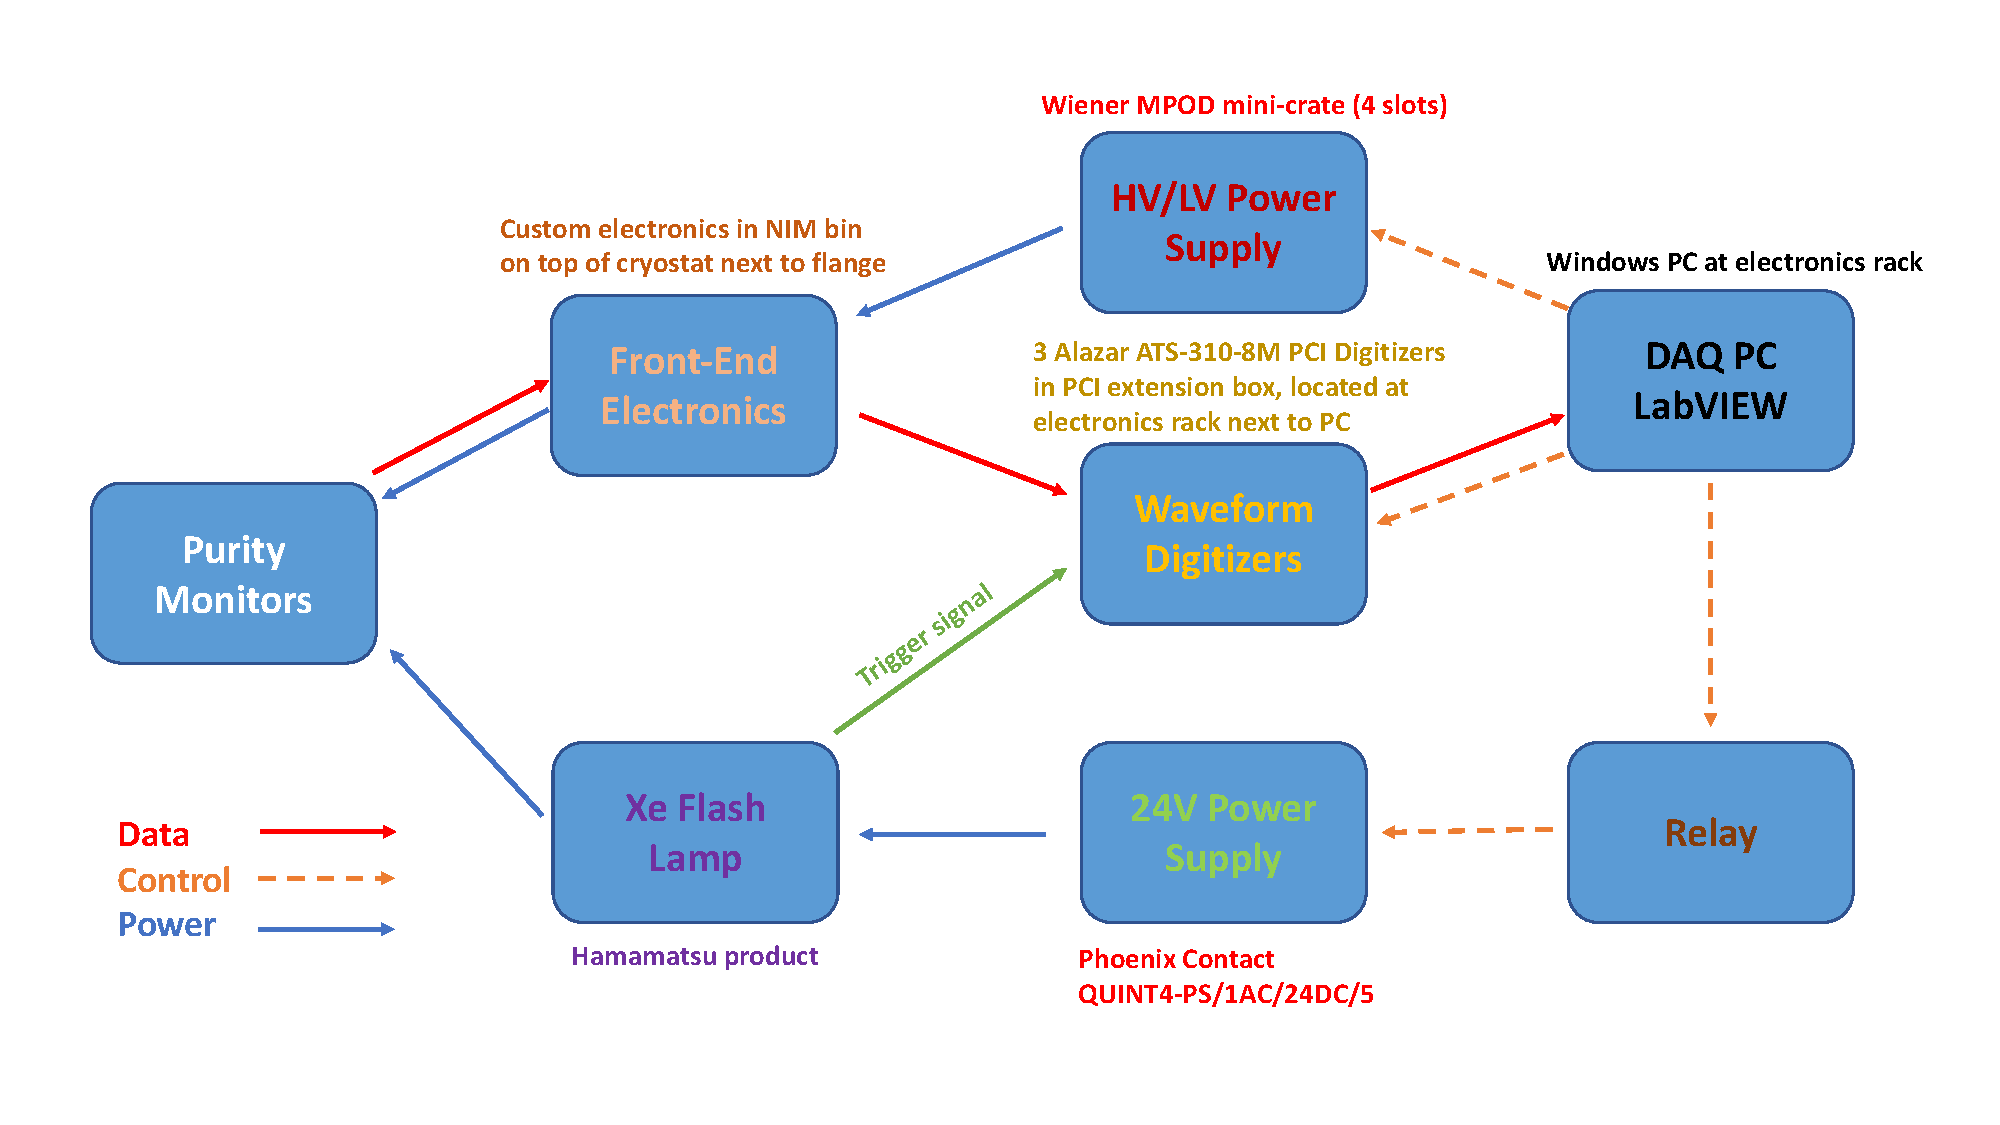
\includegraphics[width=0.9\textwidth]{PrMon_BlockDiagram.pdf}
\end{dunefigure}


The baseline design of the \dword{fe} electronics is the one used for the purity monitors at the \dword{35t}, LAPD, and \microboone. The cathode and anode signals are fed into two charge amplifiers contained within the purity monitor electronics module.
This electronics module includes a HV filter circuit and an amplifier circuit that are shielded by copper plates, so the signal and high voltage can be carried on the same cable and decoupled inside the purity monitor electronics module.
The amplified outputs of the anode and cathode are recorded with a waveform digitizer that interfaces with a \dword{daq} PC.
The shields of the signal and HV cable connect to the grounding points of the cryostat and are separated from the electronic ground with a resistor and a capacitor connected in parallel, mitigating ground loops between the cryostat and the electronics racks. The amplified outputs are transmitted to an AlazarTech ATS310 waveform digitizer that contains two input channels each with 12-bit resolution. Each channel is capable of sampling a signal at a rate of \SI{20}{\mega\samples\per\second} to \SI{1}{\kilo\samples\per\second} and storing up to \SI{8}{\mega\samples} in memory. One digitizer is used per purity monitor and each interfaces with the DAQ PC across the PCI bus. 

A custom LabVIEW application running on the \dword{daq} PC is developed and executes two functions: it controls the waveform digitizers and the power supplies, and it monitors the signals and key parameters. The application configures the digitizers to set the sampling rate, the number of waveforms to be stored in the memory, pre-trigger data, and a trigger mode. A signal from a photodiode triggered by the xenon flash lamp is directly fed into the digitizer as an external trigger to initiate data acquisition. The LabVIEW application automatically turns on the xenon flash lamp by powering a relay at the start of data taking and then turns it off when finished.
The waveforms stored in the digitizers are transferred to the DAQ PC and used to obtain averaged waveforms in order to reduce the electronic noise present in waveforms. The baseline is estimated by using the pre-trigger data and subtracted from the waveforms to measure peak voltages of the cathode and anode signals. These processes are performed in real time within the application and are then used to estimate the electron lifetime.
The application continuously displays the waveforms and important parameters, such as measured electron lifetime, peak voltages, and drift time of electrons in the purity monitors, and shows these parameters over time.
This allows one to validate the impurity of the \dword{lar} and see effects that may not be spotted at an instantaneous moment. Instead of storing the measured parameters, the waveforms and the digitizer configurations are recorded in binary form for offline analysis. ISEG HV modules in a WIENER MPOD mini crate are used to supply negative and positive voltages to the cathode and the anode, respectively. The LabVIEW application will control and monitor the HV systems through an Ethernet interface.  

The xenon flash lamp and the \dword{fe} electronics are installed close to the purity monitor flange, to reduce light loss through the optical fiber and prevent signal loss. Other pieces of equipment are mounted in a rack separate from the cryostat. They distribute power to the xenon flash lamp and the \dword{fe} electronics, as well as collect data from the electronics. The slow control system communicates with the purity monitor \dword{daq} software and has control of the \dword{hv} and \dword{lv} power supplies of the purity monitor system. As the optical fiber has to be very close to the photocathode (less than \SI{0.5}{\milli\meter}) for efficient \phel extraction, little interference with the \dword{pds} is expected. 
The electronics of purity monitors could induce noise in the \dshort{tpc} electronics, largely coming from the current surge in the discharging process of the main capacitor of the purity monitor xenon light source when producing a flash.  This source of noise can be controlled by placing the xenon flash lamp inside its own Faraday cage, allowing for proper grounding and shielding; the extent of mitigation will be evaluated at \dword{protodune}. According to the operation of purity monitors at \dword{pdsp}, after careful checks of the grounding, this noise is well below the regular noises generated by other sources.

We will use triggering to prevent any potential noises from the purity monitor's flash lamp from affecting TPC and \dword{pds} signals. The neutrino spill trigger rate is a few hertz, and each trigger window is one or a few milliseconds. For a purity monitor's flash lamp, since the flash light pulse is very short (at a microsecond level, much shorter than the gaps between LArTPC trigger windows), it is possible to send a LArTPC trigger signal to a programmable pulse generator, then let the pulse generator generate trigger pulses that do not overlap with the LArTPC trigger windows. This trigger pulse will then be sent to the external trigger port on the flash lamp HV controller to control the lamp so that it flashes in the interim times between the LArTPC trigger windows. In this way, the electronic and light noises from the flash lamp will not affect the LArTPC data-taking at all.


%If an unavoidable interference problem is found to exist, then software can be implemented to allow the \dword{daq} to know if and when the purity monitors are running and to veto purity monitor measurements in the event of a \dword{snb} alert or trigger. 

%\fixme{Nevertheless light interference will be evaluated more precisely at \dword{protodune}.}
%%%%%%%%%%%%%%%%%%%%%%%%%%%%%%%%%%%%%%%%%%
\subsubsection{Production and Assembly}
\label{sec:PrMon-Production-Assembly}
%Andrew
Production of the individual purity monitors and their assembly into the string that gets placed into the \dword{detmodule} cryostat follows the same methodology that is being developed for \dword{protodune}.  Each of the individual monitors is fabricated, assembled and then tested in a smaller test stand.  After confirming that each of the individual purity monitors operates at the required performance, they are assembled together via the support tubes used to mount the system to the inside of the cryostat such that three purity monitors are grouped together to form one string, as shown in Figure~\ref{fig:PrMon-SystemString}.

%The assembly of the individual purity monitors into the string would follow the steps laid out in the first 5 panels of Fig.~\ref{fig:PrMon-Assembly}.



\begin{dunefigure}[Design of the purity monitor string that will contain three purity monitors.]{fig:PrMon-SystemString}
  {Design of the purity monitor string that will contain three purity monitors.}
  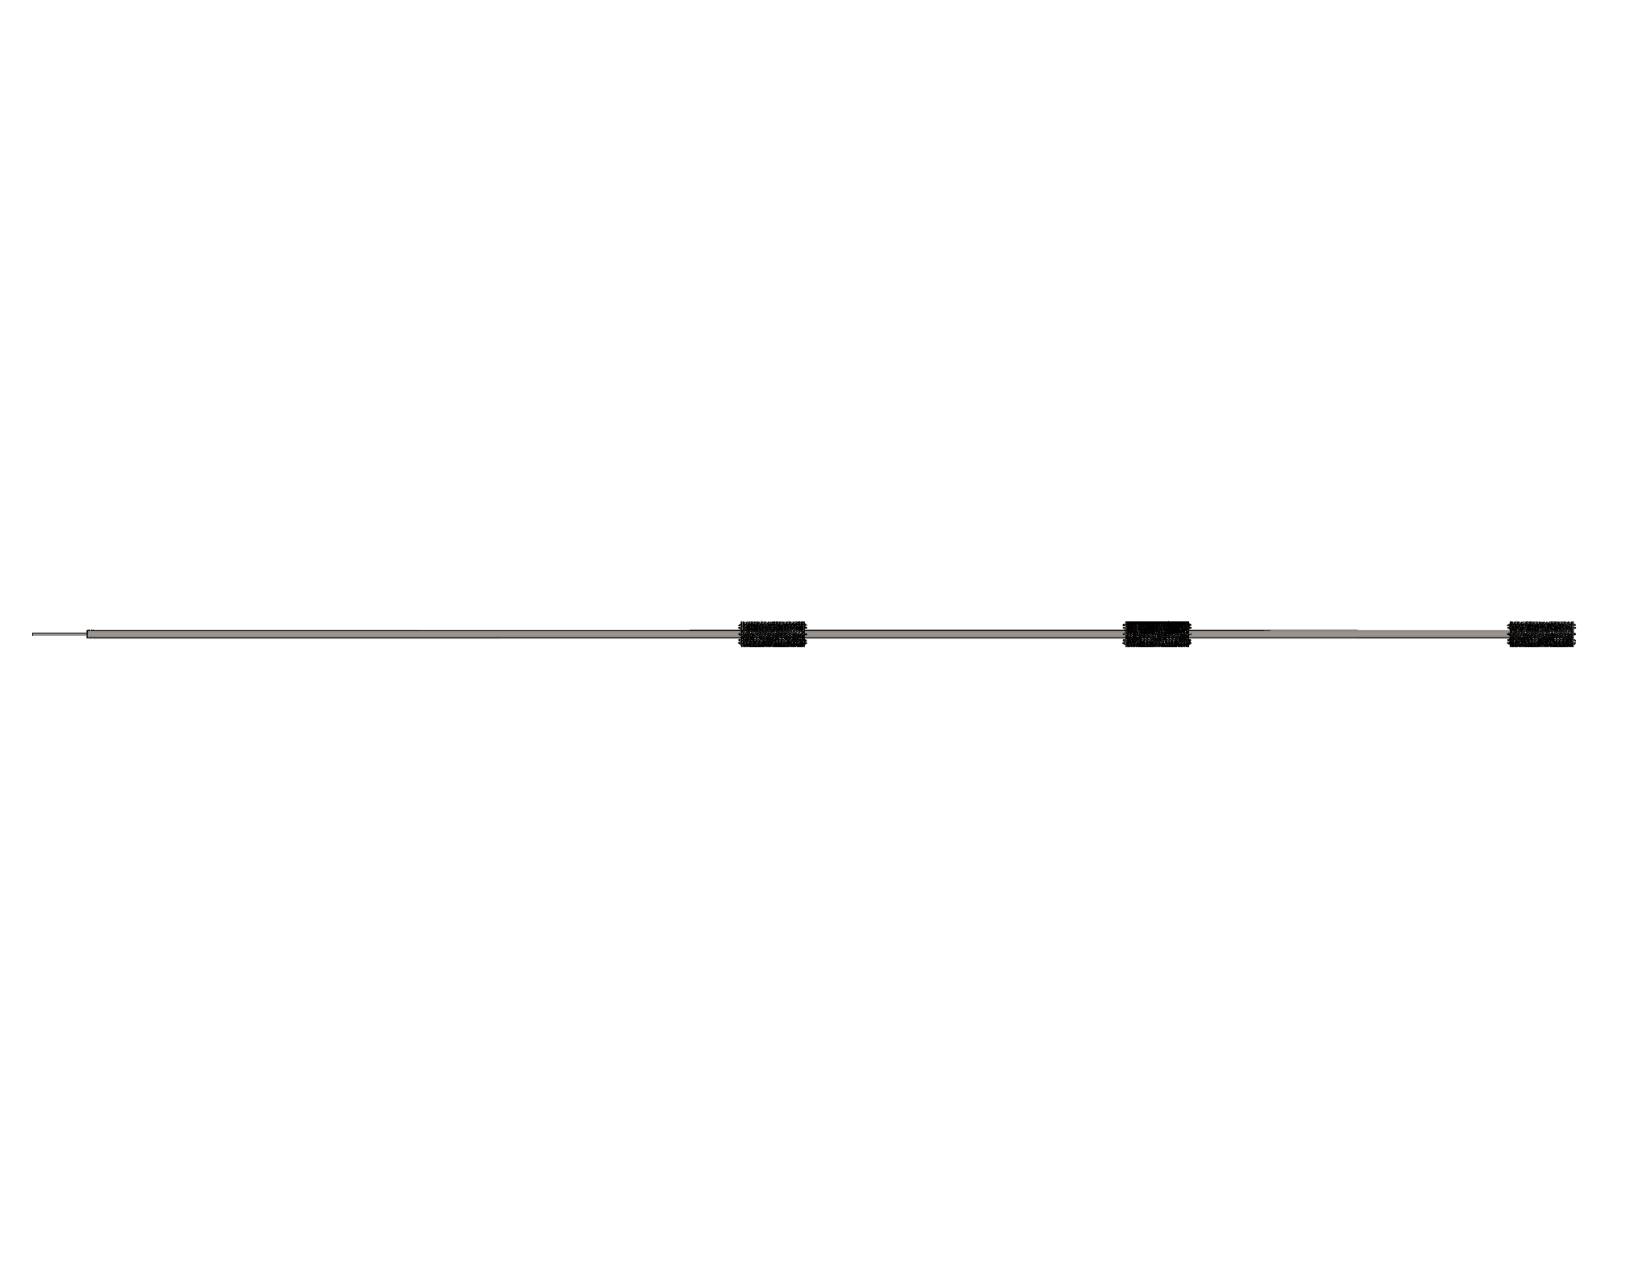
\includegraphics[width=0.9\textwidth]{PrMon-SystemString.pdf}
\end{dunefigure}



%\begin{dunefigure}[Purity Monitor String Assembly]{fig:PrMon-Assembly}
%  {Assembly sequence of the purity monitors.}
%  \includegraphics[width=\textwidth]{PrMon-Assembly.pdf}
%\end{dunefigure}



A short version of the assembly with all purity monitors will be tested in the liquid argon test facility. The full string assembly will be installed and shipped to the \dword{fd} site. A vacuum tested in a long vacuum tube will be performed onsite before inserting the full assembly into the \dword{fd} cryostat. 

%not clear if we want to ship the 12 meter assembly or assemble onsite yet.
%Each monitor is assembled as the string is built from the top down, and in the end %there would be 
%three individual purity monitors %hanging 
%hang from a single string.  The assembly of the string concludes once the purity monitors are each in %place, but with the Faraday cages removed and the \dword{hv} cables and optical fibers yet to be run.  
%This full string assembly is then %would then be 
%shipped to the \dword{fd} site for installation into the cryostat. // a shorter version need to be tested in the LAr testing facility



\subsection{Thermometers}
\label{sec:fdsp-cryo-therm}
As mentioned above, a detailed 3D temperature map is important to monitor the correct functioning of the cryogenic system and the LAr uniformity.
Given the complexity and size of purity monitors, those can only be installed on the cryostat sides to provide a local measurement of
the LAr purity. While a direct measurement of the LAr purity across the entire cryostat is not viable, a sufficiently detailed 3D temperature map
can be used to predict the LAr purity using CFD simulations. Specially important is the vertical coordinate since this will be closely related to
the LAr recirculation and uniformity. 

The baseline sensor distribution, as well as the cryostat ports used to extract cables (with indication of number of cables per port), is shown in figure~\ref{fig:cisc-tsensor-map}. This distribution will evolve when more information will be available (precise CFD simulations, better understanding of DSS ports, installation interfaces with other groups), but it is sufficient to establish the overall strategy.

\begin{dunefigure}[Distribution of temperature sensors inside the cryostat]{fig:cisc-tsensor-map}
  {Distribution of temperature sensors inside the cryostat}
  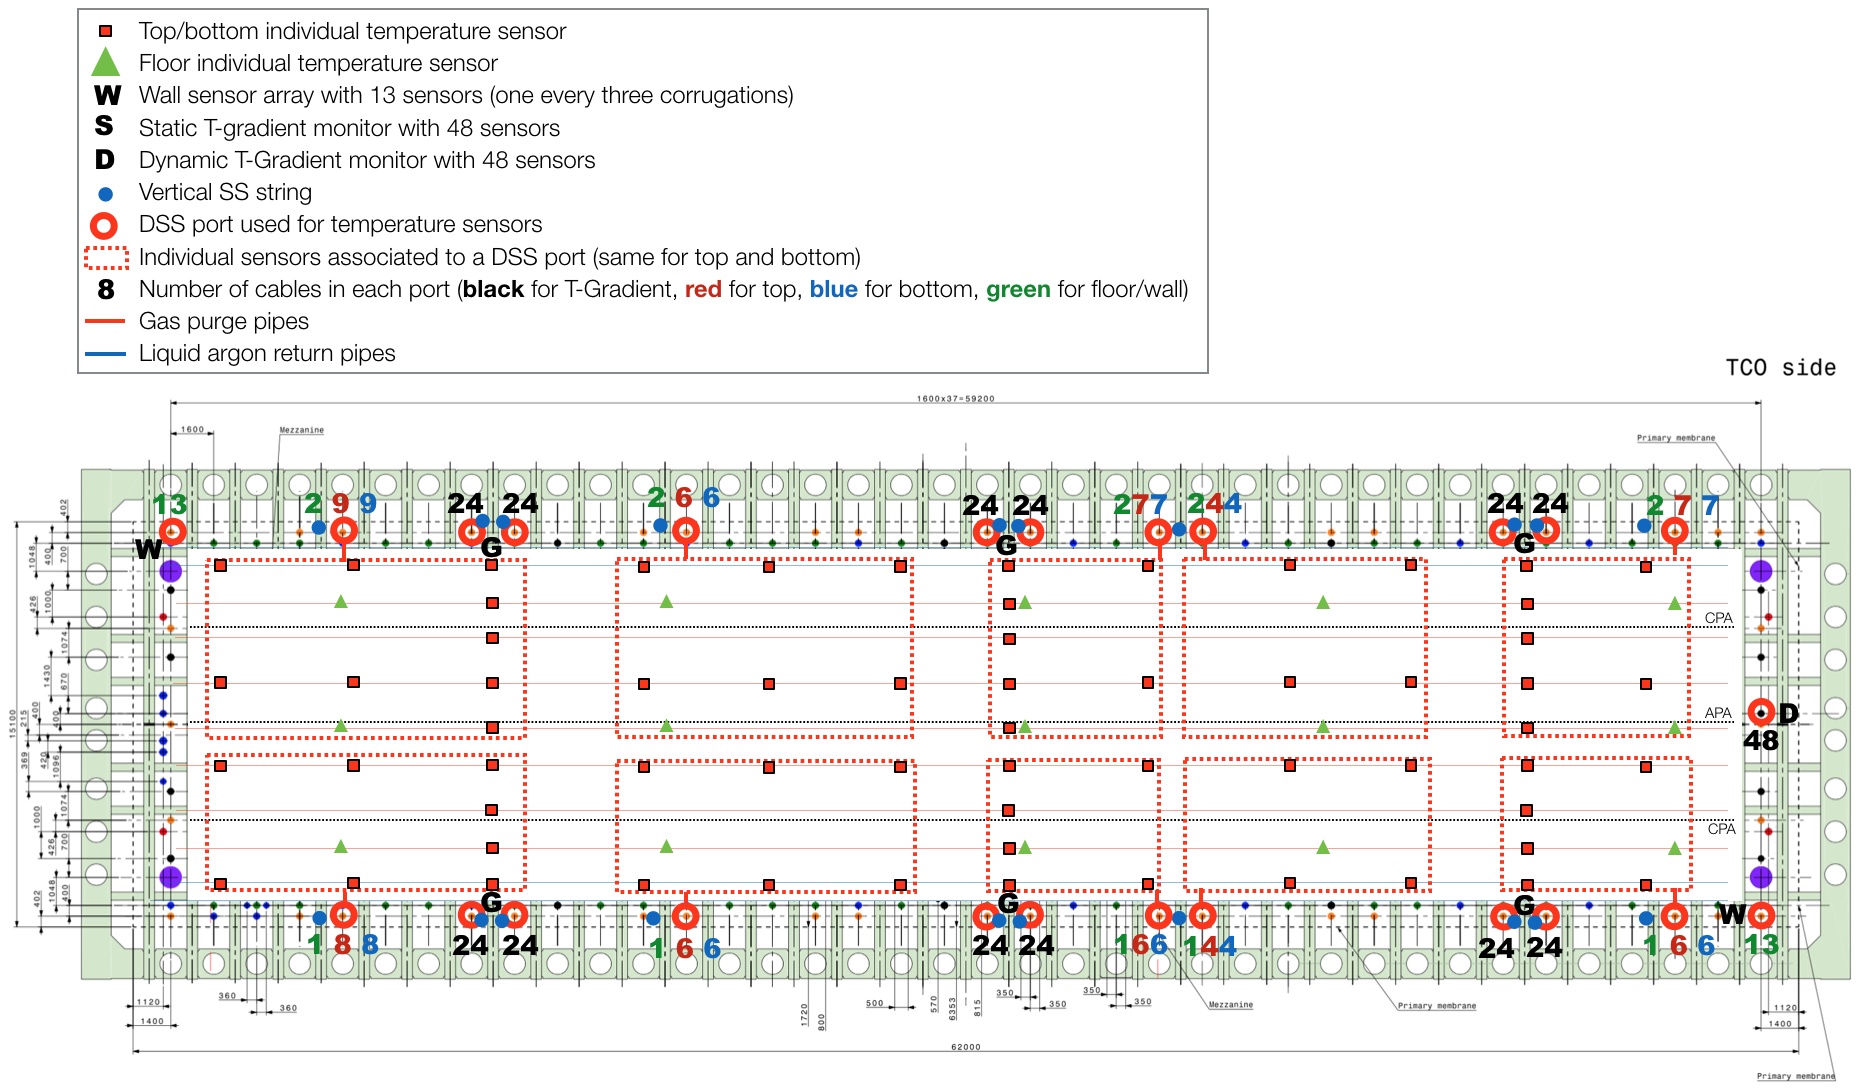
\includegraphics[width=0.9\textwidth]{cisc_tsensor_map.png}
\end{dunefigure}

High precision temperature sensors will be distributed near the TPC walls in two ways:
i) forming high density (\(>2\) sensors/\si{m}) vertical arrays (the so-called T-gradient monitors), and ii) in coarser ($\sim$ 1 sensor/\SI{5}{m}) 2D arrays 
at the top and bottom of the detector, which are the most delicate regions (the so-called individual sensors). 

Since temperature variations inside the cryostat are expected to be very small ($\SI{0.02}{K}$, see Fig.~\ref{fig:cfd-example}) %\todo{Missing figure in Thermometers intro --> \textbf{Anselmo(?) to copy figure from IDR.}}, to properly measure the 3D temperature map 
sensors must be cross-calibrated to better than $\SI{0.005}{K}$. Most sensors will be calibrated in the laboratory, prior to installation,
as described in the next section. This is in fact the only viable method for sensors in areas where the available space is restricted: on the long sides of the detector
% (behind the APAs for SP, and behind the lateral FC end-walls for DP) 
and top/bottom of the detector.
Given the precision required and the unknown longevity of the sensors, which could require a new calibration after some time, a complementary method
will be used for T-gradient monitors behind the front end-walls.
% at least for the SP detector.
In those areas there is sufficient space for a movable system, which can be used to cross calibrate
the temperature sensors  {\em in situ}. This calibration method is described in the section about dynamic T-gradient monitors. 

In the baseline design for all three systems mentioned above three elements are common: sensors, cables and readout system.
Platinum sensors with \SI{100}{\ohm} resistance (PT100 series), produced by Lakeshore,  
are adequate for the temperature range of interest, 83-92\si{K}, since in this range those sensors have high reproducibility 
$\sim\SI{5}{mK}$ and absolute temperature accuracy of \SI{100}{mK}.
The use of 4-wire readout will greatly reduce the issues related to the lead resistance, any parasitic resistances,
connections through the flange and general electromagnetic noise pick-up. The Lakeshore PT102 sensors
%(see Fig.~\ref{fig:sensor_cable}-Left)
have being previously used in the 35t prototype and ProtoDUNE-SP detector,
giving excellent results. For the inner readout cables a custom cable made by Axon is the baseline. It consists in four teflon-jacketed 
copper wires (AWG28), forming two twisted pairs, with an metallic external shield
and an outer teflon jacket.
%Further details are given in Fig.~\ref{fig:sensor_cable}-Right. 
The readout system will be described below in a separate subsection. 

%As shown in Fig.~\ref{fig:sensor_cable}, the PT102 sensor has a length of \SI{21}{mm}, which can easily be accommodated in the DUNE T-gradient monitors. 

%\begin{dunefigure}[DUNE baseline choices for sensor and cable]{fig:sensor_cable}
%  {DUNE baseline choices for sensor and cable. Left: Schematic diagram of the PT102 sensor from the Lakeshore company. Right: Schematic diagram and properties of the four wires cable from the
%  Axon company}
%  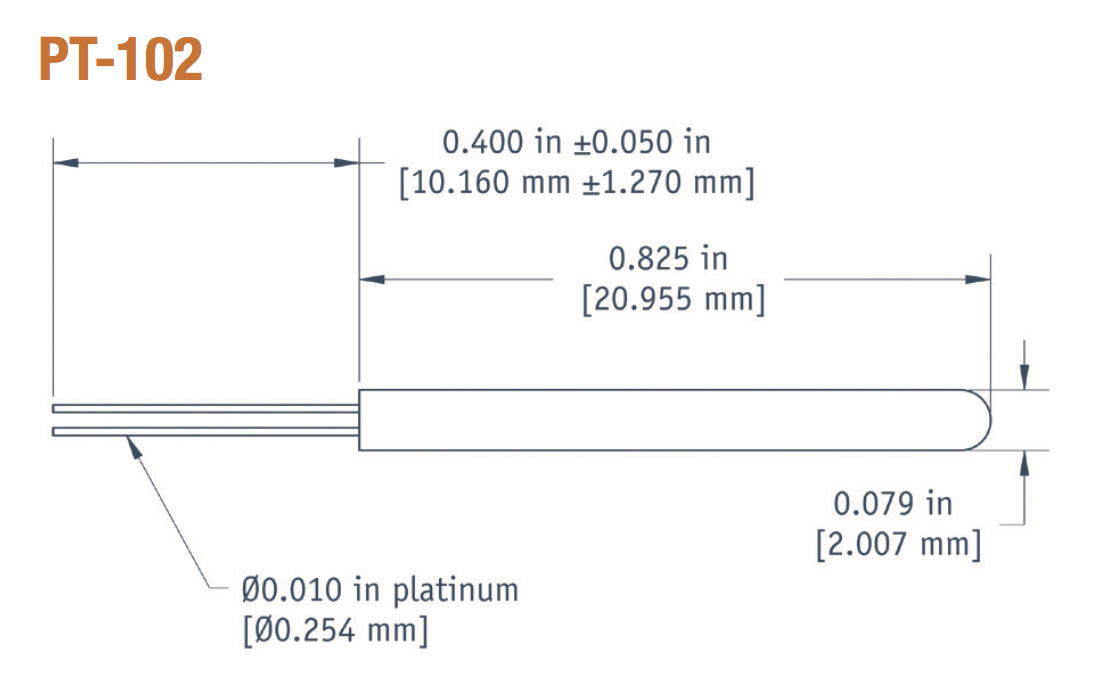
\includegraphics[width=0.4\textwidth]{cisc_pt102.png}
%  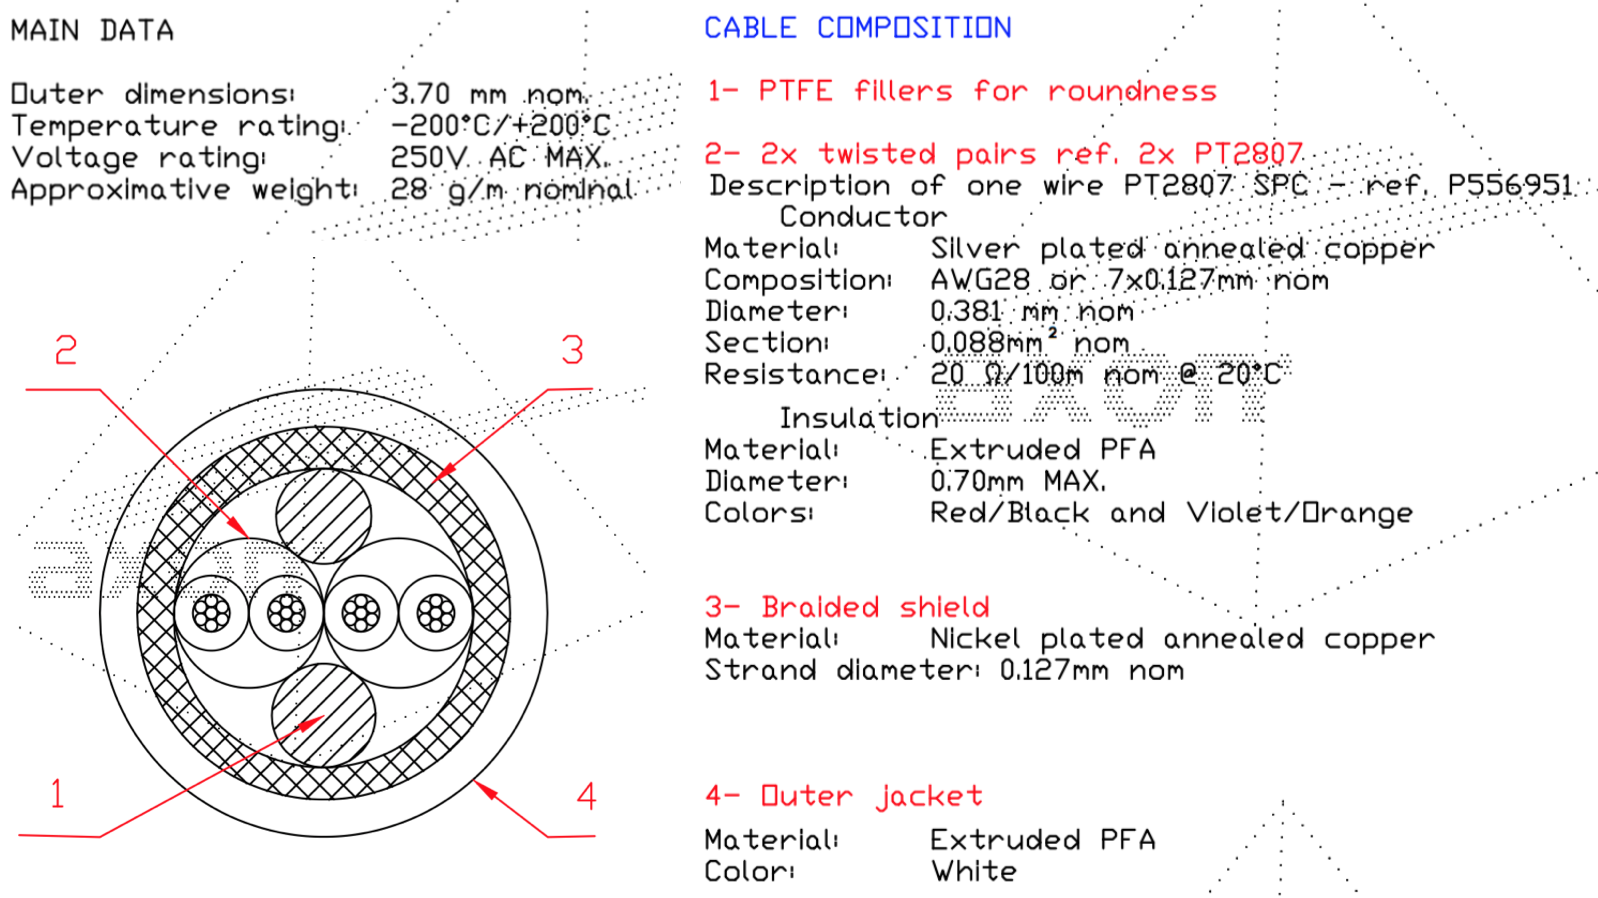
\includegraphics[width=0.55\textwidth]{cisc_TAxonCable.png}
%\end{dunefigure}

Another set of lower precision sensors epoxied into the cryostat bottom membrane will be used to monitor the filling of the cryostat in its initial stage.   
Finally, the inner walls and roof of the cryostat will be instrumented with the same type of sensors in order to monitor their temperature during cool-down and filling (W sensors in figure~\ref{fig:cisc-tsensor-map}).
 
% \fixme{Remove references to DP -- done}
 
%except for the membrane sensors that may come from Minco.

% % % %
\subsubsection{Static T-Gradient monitors}

Several vertical arrays of high precision temperature sensors cross-calibrated in the laboratory will be installed behind the APAs.  
% near the lateral walls.
%(behind the APAs for SP and behind the lateral FC end-walls for DP). 
%For the SP detector, since the electric potential is zero behind the APAs, no electric field shielding is required, simplifying enormously the mechanical design.
%\footnote{This does not apply for the DP detector, for which the proper shielding must be provided.} 
The baseline design assumes six arrays with 48 sensors each. Spacing between sensors
is 20 cm at the top and bottom and 40 cm in the middle area. This configuration is similar to the one used in \dword{pdsp} but with nearly double spacing. As shown in Fig. \ref{fig:cisc-cfd-valid} a configuration with 48 sensors seems appropriate in \dword{pdsp} as it should be in DUNE where the expected total gradient is not larger (see Fig.~\ref{fig:cfd-example}). 

\begin{dunefigure}[Temperature sensor resolution and reproducibility]{fig:Trepro}{
 Left:   Temperature offset between two sensors as a function of time for four independent immersions in LAr. The reproducibility of those sensors, defined as the RMS of the mean offset in the flat region, is $\sim \SI{1}{mK}$,
    The resolution for individual measurements, defined as the RMS of one of the offsets in the flat region, is better than \SI{0.5}{mK}. Right: Difference between the mean offset obtained with two independent calibration methods for the 51 sensors calibrated. The standard deviation of this distribution is taken as precision of the calibration.}
  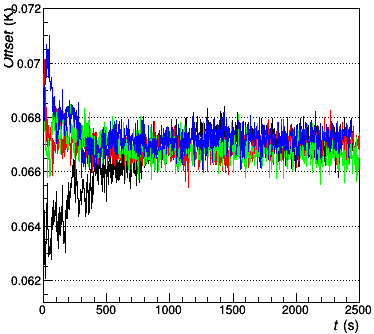
\includegraphics[height=0.44\textwidth]{cisc_tsensor_calib.png}%
  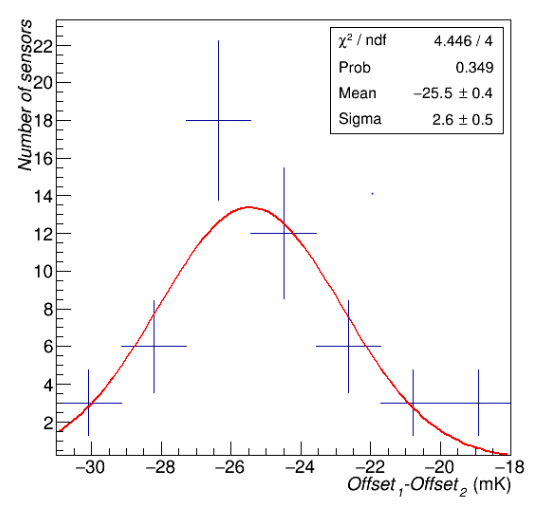
\includegraphics[height=0.45\textwidth]{cisc_tsensor_calib2.png}%
\end{dunefigure}

Sensors are cross-calibrated in the lab using a well controlled environment and a high precision readout system, described below in a separate subsection.
%Although the calibration procedure will certainly improve, the one currently used for ProtoDUNE-SP is descrived here.
%Four sensors are placed as close as possible (such that identical temperature can be assumed for all of them) inside a small cylindrical aluminum capsule,
%which protects the sensors from thermal shocks and helps in minimizing convection.
%One of the sensors acts as reference while the other three are the ones being calibrated. Five independent calibrations
%are performed for each set of three sensors, such that the reproducibility of each sensor can be computed. For each calibration 
%the capsule is introduced in a PLA box of size \(9.5\times9.5\times\SI{19}{cm^3}\), with two concentrical independent volumes of LAr
%and sourounded by a polystyrene box with \SI{15}{cm} thick walls. A small quantity of LAr is used to slowly
%cooldown the capsule to $\sim\SI{90}{K}$, avoiding thermal shocks that could dammage the sensors.
%Then the capsule is covered by LAr such that it penetrates
%inside fully covering the sensors. Once the temperature stabilizes to the 1-\SI{2}{mK} level (after 5-15 minutes) measurements are taken. Then the capsule is taken out from LAr
%and kept at room temperature until it reaches \SI{200}{K}. As mentioned above, this procedure is repeated five times, before going to the next set of three sensors.  
As shown in figure ~\ref{fig:Trepro} a precision of $\SI{2.6}{mK}$ has been achieved in the calibration of ProtoDUNE-SP sensors. This has been confirmed with ProtoDUNE-SP temperature data, as shown in figure~\ref{fig:cisc-cfd-valid}), where the difference in temperature measured by two adjacent sensors is consistent with the claimed precision.  


\begin{dunefigure}[Conceptual design of the Static T-Gradient monitor]
{fig:cisc-static-tgradient}
  {Conceptual design of the Static T-Gradient monitor.}
  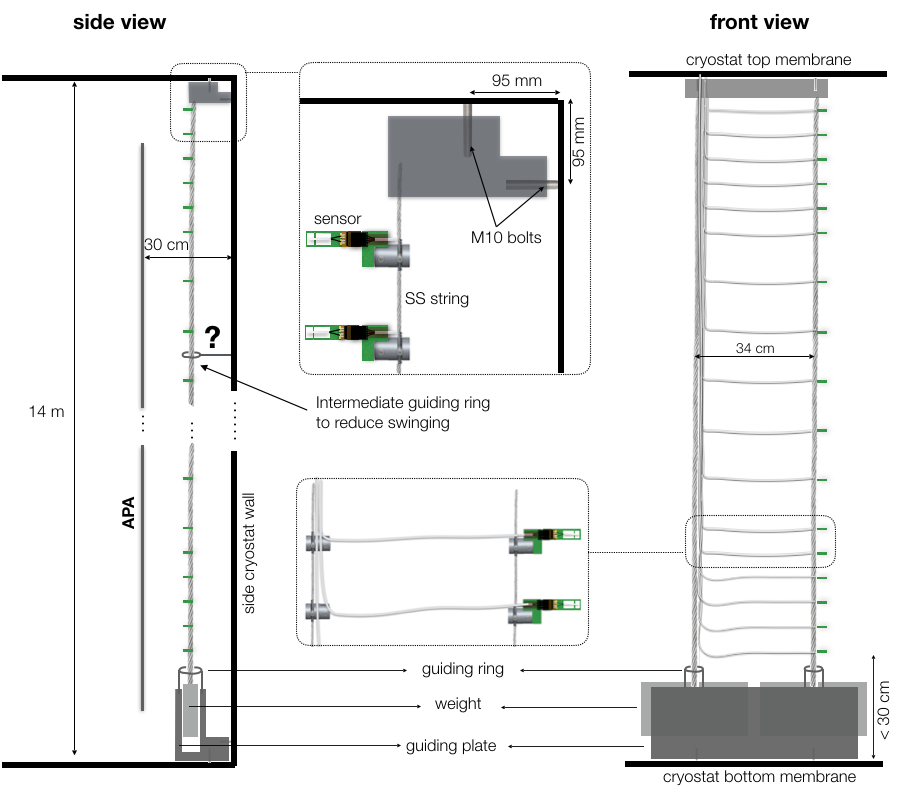
\includegraphics[width=0.8\textwidth]{cisc_static_tgradient.png}
\end{dunefigure}

The baseline design for the mechanics 
%of the SP system 
is shown in figure~\ref{fig:cisc-static-tgradient}. It consists in two stainless steel strings anchored at top and bottom corners of the cryostat
using the available M10 bolts (see Fig.~\ref{fig:sensor-support}-Left). One of the strings is used to route the cables while the other,
separated \SI{340}{mm}, serves as support for temperature sensors.
Given the height of the cryostat, the need of an intermediate anchoring point to reduce swinging is under discussion. To account for the shrinkage of the strings under cryogenic conditions and to guaranty that the same tension is always applied a weight at the bottom of the strings is used. A guiding system made of stainless steel and anchored at four bottom M10 bolts is used to keep the weight confined in space. A prototype is being built at IFIC, where the full system will be mounted using two dummy cryostat corners. An alternative design with carbon fiber strings is also under consideration.  

% \fixme{Static T-Gradient: comment out reference to dual phase? [gahs] --- I took the liberty of doing this myself [gahs]}
% For the DP detector no baseline design exists yet,
% since additional complications due to the required electric field shielding must be taken into account. 
% \todo{Is the second sentence in this paragraph about dual phase? Why does paragraph begin with dual phase? [gahs]}

Fig.~\ref{fig:sensor-support}-Right shows the baseline design of the
PCB support for temperature sensors, with an IDC-4 male connector. 
It has a size of $52\times \SI{15}{mm^2}$. A narrower connector (with two rows of two pins each) is currently under study. This alternative design would reduce the width of the PCB assembly and allow for an increase in the number of sensors calibrated simultaneously. Each four-wires cable from the sensor to the flange will have an IDC-4 female connector on the sensor side; on the other side, it will be soldered/crimped to the appropriate connector, whose type and number of pins (SUBD-25 connectors where used in ProtoDUNE-SP) depends on the final design of the DSS ports,
which will be used to extract the cables. 

\begin{dunefigure}[Cryostat bolts and temperature sensor support]{fig:sensor-support}
  {Left: bolts at the bottom corner of the cryostat. Right: Lakeshore PT102 sensor mounted on a PCB with an IDC-4 connector.}
  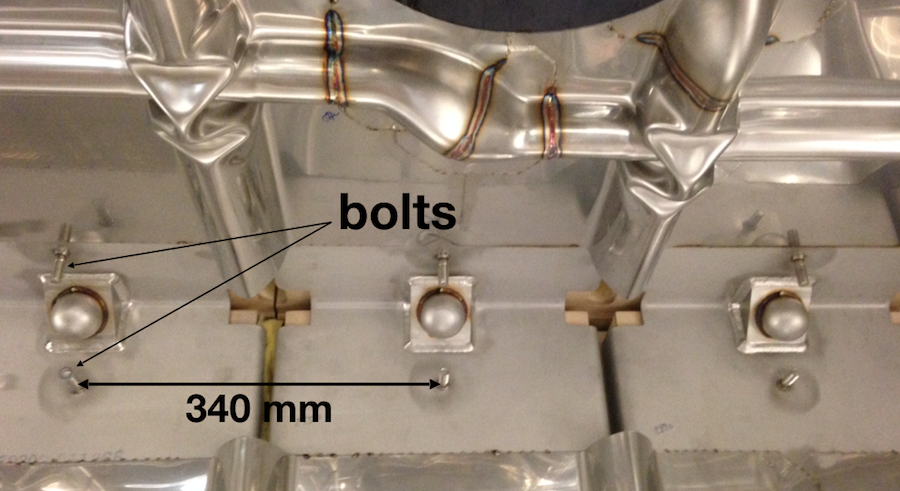
\includegraphics[height=0.2\textwidth]{cisc_cryostat_bolts.png}%
    \hspace{1cm}%
  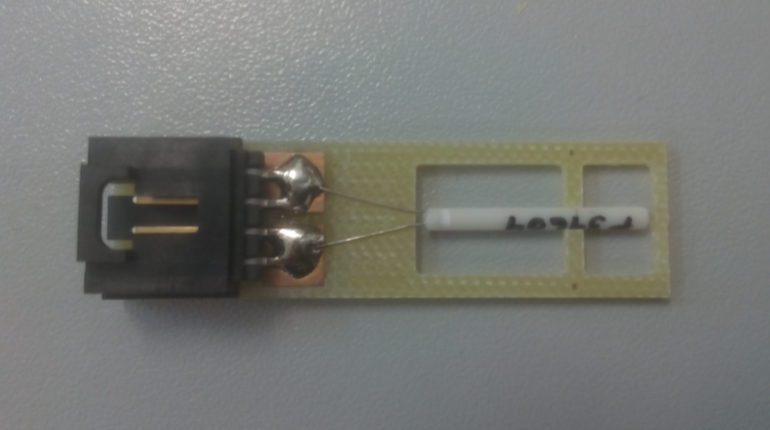
\includegraphics[height=0.2\textwidth]{cisc_tsensor.png}%
\end{dunefigure}




% \begin{dunetable}
% [Static t-gradient parameters]
% {p{0.2\textwidth}p{0.1\textwidth}p{0.6\textwidth}}
% {tab:fdgen-cisc-static-tgradient}
% {Parameters for the Static T-gradient monitor}   
% Parameter            & {\bf value} & {\bf comment} \\ \toprowrule
% \# sensors	         &     48      &       \\ \toprowrule
% sensor spacing       &    20/40 cm & 20 at top and bottom and 40 in the mid area  \\ \toprowrule
% cable diameter       &   3.5 mm    &       \\ \toprowrule
% cable weight         &   28 g/m    &       \\ \toprowrule
% cable-string weight  &   13 Kg     &  10 Kg for the cable, 1.3 Kg for the SS string and 1.7 kg for the cable supports      \\ \toprowrule
% sensor-string weight &   3.3 Kg     & 1.3 Kg for the SS string, 1.7 kg for the cable supports and 300 g for the sensors     \\ \toprowrule
% \end{dunetable}

%Table \ref{tab:fdgen-cisc-static-tgradient} summarizes key properties of the static T-gradient monitor.

% % % %
\subsubsection{Dynamic T-Gradient monitors}

% What I was thinking about is to have 3 sensors per meter. 4 would be even better and have 1.35 m range of motion. The goal is to have 4 sensor overlap. In this case, we would be quite safe against sensor failure.
% If we are to populate 14 m with 3 sensors per meter, that would be 42 sensors. In addition, we should increase frequency at the top or bottom.

Dynamic temperature monitor is a vertical array of high precision temperature sensors with the goal of measuring vertical temperature gradient with precision of few mK. The design of the system is driven by two factors:
\begin{itemize}
\item
few mK uncertainty in the measured vertical temperature profile over the entire detector height is required to monitor LAr purity and provide useful feedback of efficiency cryogenic recirculation and purification.
\item
simulations of the cryogenic recirculation predict very slow change in temperature at meter scale except at the bottom and top of the cryostat. Thus, sensors will be placed every \SI{50}{cm} along the detector height with increased frequency in the first \SI{50}{cm}, closest to the bottom of the cryostat and the last \SI{50}{cm}, closest to the top of the cryostat, where spacing between sensors is reduced to \SI{10}{cm}.
 \end{itemize}


 In order to address concerns related to potential difference in the sensor reading prior to installation and after installation in DUNE FD dynamic temperature monitor allows cross-calibration of sensors in situ. Namely, this T-gradient monitor  can move vertically while installed in DUNE FD, which allows for precise cross-calibration between the sensors in-situ at predefined locations as well as in between them. The procedure for cross-calibrations is the following: the temperature reading is taken at the lowest position with all sensors. Then, the stepper motor moves the carrier rod up for \SI{50}{cm} putting all sensors in the location of their neighbor that is \SI{50}{cm} above them. Then the second reading is taken. In this manner, except for the lowest position we have temperature measurement at each location with two adjacent sensors, and by linking the temperature offsets between the two readings at each location, temperature readings from all sensors are cross-calibrated in situ, canceling all offsets due to electromagnetic noise or any parasitic resistances that may have prevailed despite the four point connection to the sensors that should cancel most of the offsets. These measurements are taken with very stable current source, which ensures high precision of repeated temperature measurements over time. The motion of the dynamic T-monitor is stepper motor operated, delivering measurements with high spatial resolution. 

This concept has been already tested in ProtoDUNE-SP, where the system has been successfully moved up by a maximum of 51 cm allowing for the cross-calibration of all sensors (22 sensors with 10.2 cm spacing at top and bottom and 51 cm in the middle). 
The temperature profile after calibration was shown in Fig.~\ref{fig:cisc-cfd-valid}, whose smoothness demonstrates the reliability of the method.  

\todo{Figure on the dynamic profiler movement  to be inserted when available. }

\subsubsection{Dynamic T-gradient monitor design}
Dynamic T-gradient monitor consists of three distinct parts: carrier rod on which sensors are mounted, enclosure above the cryostat housing the space that allows vertical motion of the carrier rod 1.5\,m above its lowest location, and motion mechanism. The motion mechanism consists of a stepper motor connected to a gear and pinion motion mechanism through ferrofluidic dynamic seal. The sensors have two pins that are soldered to a printed circuit board (PCB). Two wires are soldered to the common soldering pad for each pin, individually.   There is a cutout in the PCB around the sensor that allows free flow of argon for more accurate temperature reading.  Stepper motors typically have very fine steps allowing high precision positioning of the sensors.  Figure~\ref{fig:fd-slow-cryo-dt-monitor-overview} shows the overall design of the dynamic T-gradient monitor with the sensor carrier rod, enclosure above the cryostat and stepper motor mounted on the side of the enclosure. The enclosure consists of two parts connected by 6-cross flange. One side of the 6-cross flange will be used for the signal wires, another side will be used as a viewing window, while the two other ports will be spares. Figure~\ref{fig:fd-slow-cryo-sensor-mount}-Left shows the mounting of the PCB board on the carrier rod and mounting on the sensor on the PCB along with the four point connection to the signal readout wires. Finally, Figure~\ref{fig:fd-slow-cryo-sensor-mount}-Right shows the stepper motor mounted on the side of the rod enclosure. The motor is kept outside, at room temperature and its power and control cables are also kept outside.

\begin{dunefigure}[Dynamic T-gradient monitor overview]{fig:fd-slow-cryo-dt-monitor-overview}
  {An overview of the dynamic T-gradient monitor.}
% 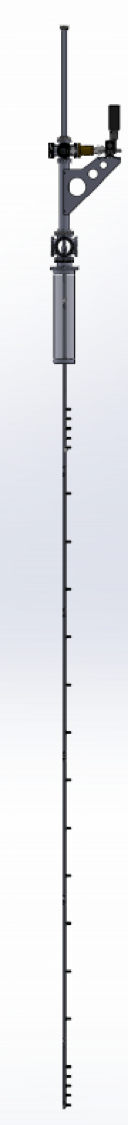
\includegraphics[width=0.11\textwidth,angle=90]{cisc_DTOverview.png}
 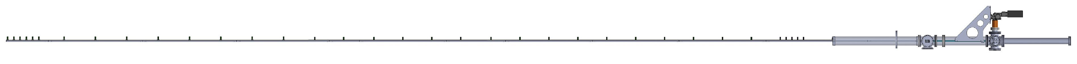
\includegraphics[width=0.95\textwidth,angle=0]{cisc_DynamicProfiler.png}
\end{dunefigure}
\begin{dunefigure}[Sensor-cable assembly for dynamic T-gradient monitor]{fig:fd-slow-cryo-sensor-mount}
  {Left: Sensor mounted on a PCB board and PCB board mounted on the rod. Right:
    The driving mechanism of the dynamic T-gradient monitor. It consists of a stepper motor driving the pinion and gear linear motion mechanism. }
  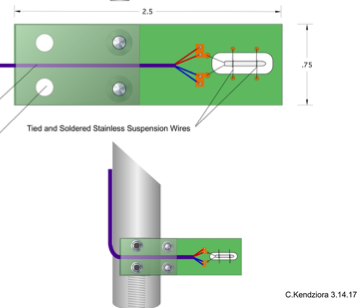
\includegraphics[width=0.40\textwidth]{cisc_DTSensorMount.png}
  \hspace{3cm}%
  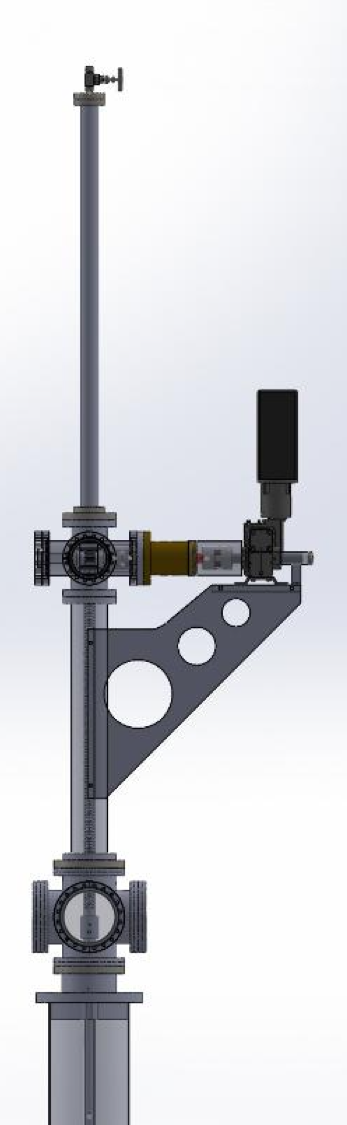
\includegraphics[width=0.12\textwidth]{cisc_DTMotor.png}
\end{dunefigure}

% % % %
\subsubsection{Individual Temperature Sensors}

T-Gradient monitors will be complemented by a coarser 2D array (every 5 m) of precision sensors at the top and bottom of the detector, as shown in figure~\ref{fig:cisc-tsensor-map}. Following ProtoDUNE-SP design, bottom sensors will use the cryogenic pipes as support structure, while top sensors will be anchored to the ground planes. Although a similar distribution of sensors at top and bottom will be pursued, small differences will come from the different distribution of suitable anchoring points. 

As in ProtoDUNE-SP, another set of standard sensors will be epoxied to the bottom membrane evenly distributed. Those will be used to detect the presence of LAr when cryostat filling starts. Finally, two vertical arrays of standard sensors will be epoxied to the lateral walls in two opposite vertical corners, with a spacing of 102 cm (every 3 corrugations), with the aim of monitoring the cryostat membrane temperature during the cool-down and filling processes. 

While in ProtoDUNE-SP cables were routed individually (not touching neighbor cables nor any metallic elements) to prevent grounding loops in the case the outer Teflon jacket was broken, it has been demonstrated that this failure mode is very unlikely to occur. Thus, in DUNE far detectors cables will be routed in bundles, simplifying enormously the design. As shown in figure~\ref{fig:cisc-tsensor-map} a maximum of 20 sensors will use the same DSS port, which corresponds to a cable bundle diameter of 16 mm.

Cable bundles of several sizes will be configured using custom made Teflon 
pieces,  %(see Fig.~\ref{fig:cable-support})
which will be anchored to different cryostat and detector elements to route cables from sensors to DSS ports. For sensors at the bottom (on pipes and floor), cables will be routed towards the cryostat bottom horizontal corner using stainless steel split clamps anchored to pipes (successfully prototyped at \dword{pdsp}), and from there towards the top of the cryostat using vertical strings (as for the static T-gradient monitors). For sensors on the top ground planes, cables bundles will be routed to the corresponding DSS port using Teflon supports attached to both the FR4 threaded rods in the union between two ground plane modules and to the DSS I-bins (both successfully prototyped at \dword{pdsp}). Sensors on the walls will use bolts in the vertical corners for cable routing. 

For all individual sensors, PCB sensor's support, cables and connection to the flanges will be the same as for the T-gradient monitors. 
  

%\begin{dunefigure}[Cable supports for individual temperature sensors]{fig:cable-support}
%  {Left: support for two cables on ground planes. Right: Supports for three %cables  mounted on cryogenics pipes using split clamps}
% This PDF is made from the .dot of the same name.
%  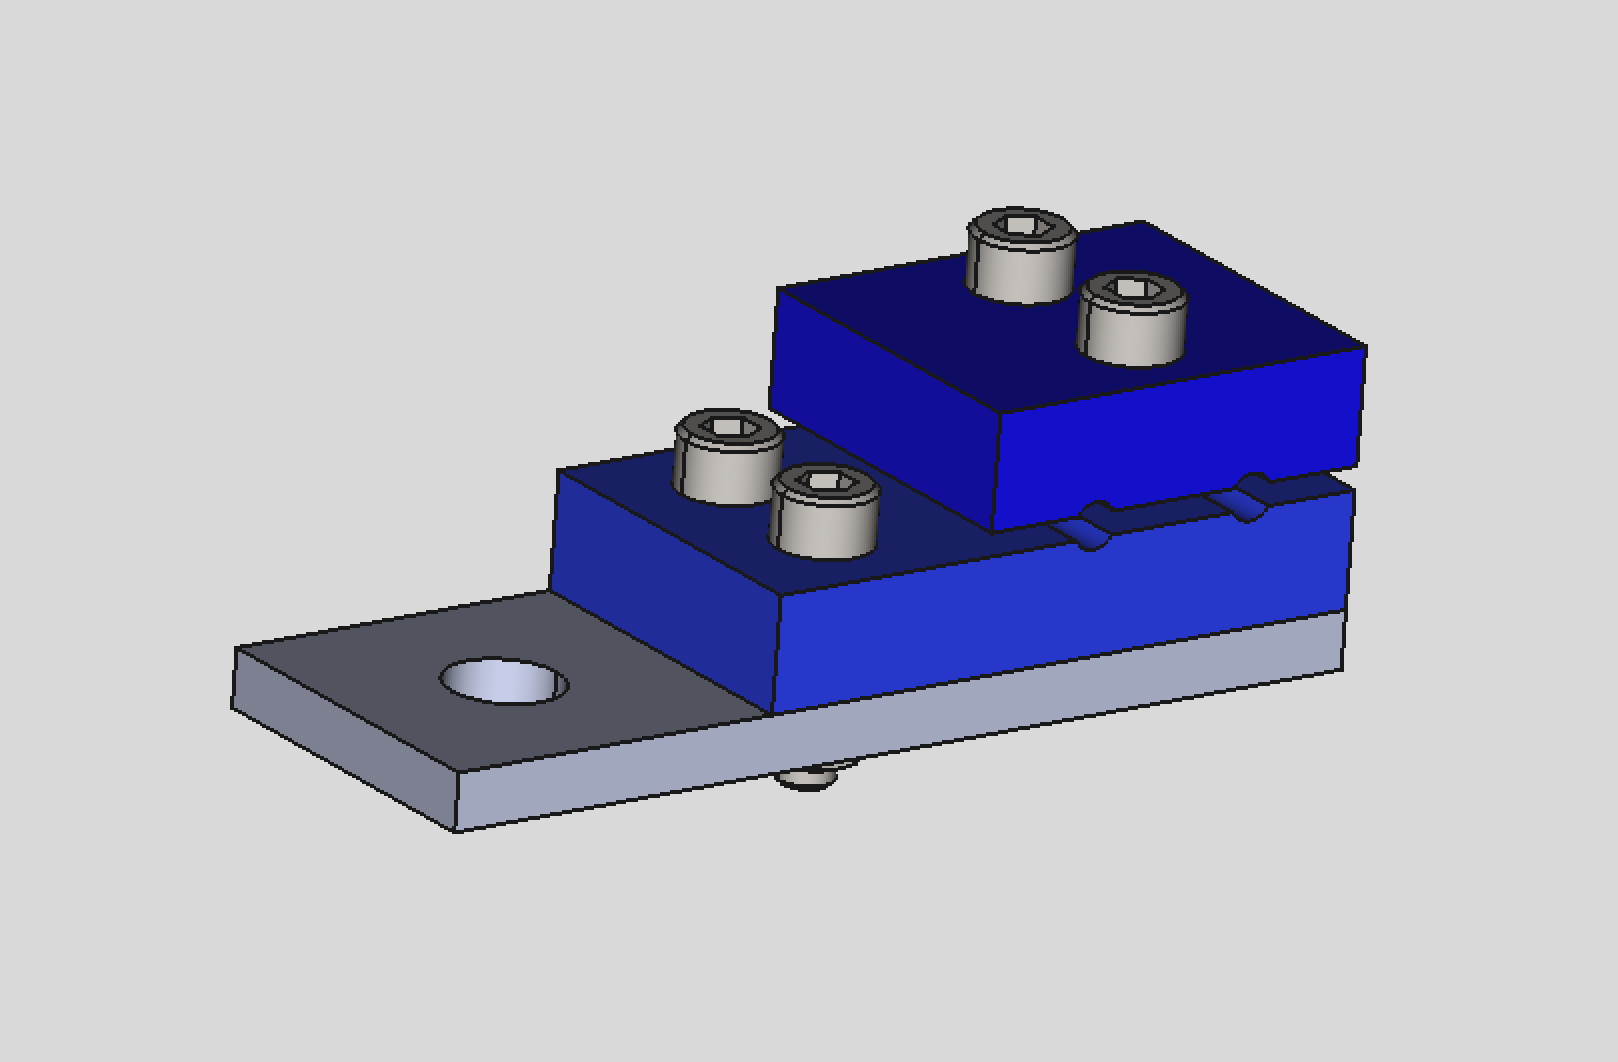
\includegraphics[width=0.3\textwidth]{cisc_TcableSupportGP.png}
%  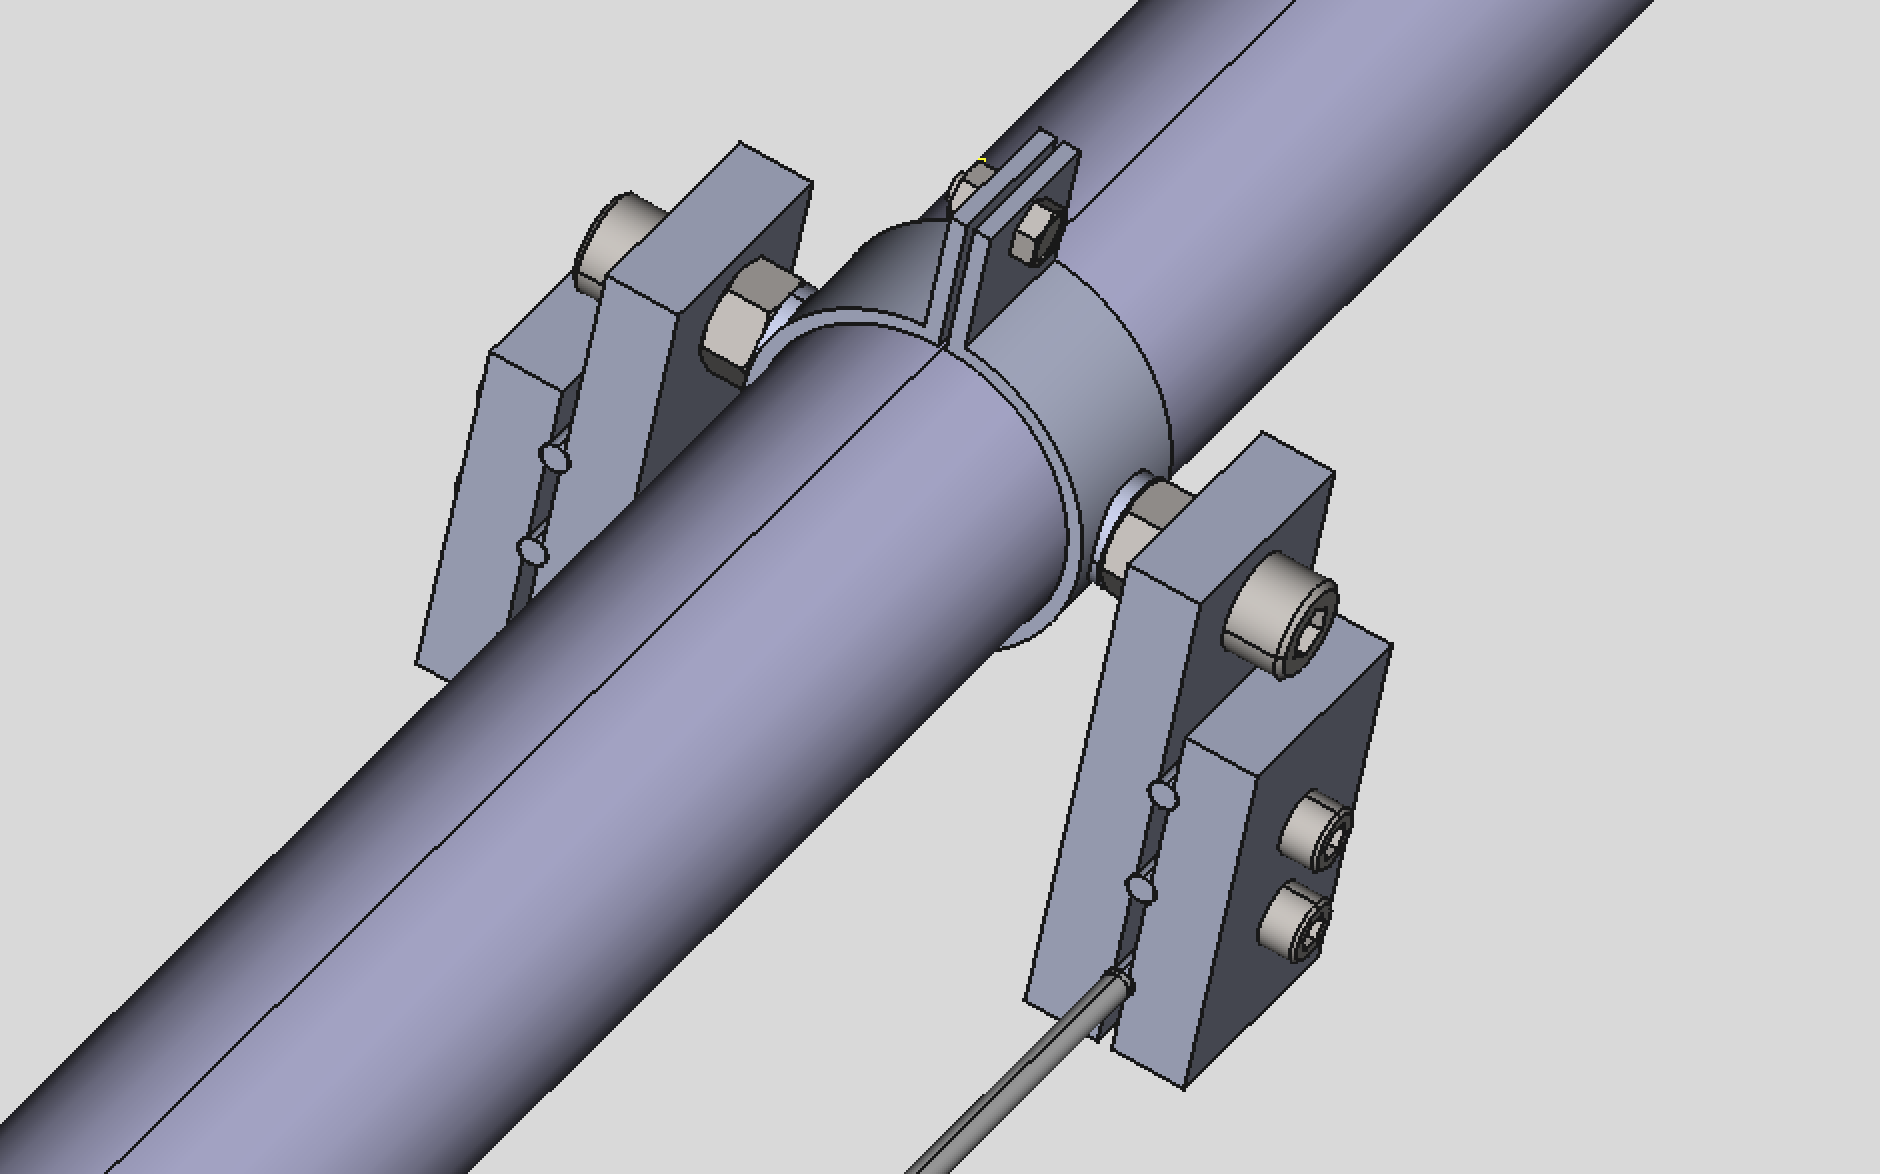
\includegraphics[width=0.315\textwidth]{cisc_TcableSupportPipes.png}
%\end{dunefigure}


% % % %
\subsubsection{Readout system for thermometers}
\label{sec:fdgen-slow-cryo-therm-readout}

A high precision and very stable system is required to achieved the design precision of $< \SI{5}{mK}$.
The proposed readout system is the one used in ProtoDUNE-SP, which relies on a variant of an existing mass PT100 temperature readout system developed at
CERN for one of the LHC experiments; prior  test and validation by the collaboration experts. The system consists in an electronic circuit which includes:
\begin{itemize}
\item A precise and accurate current source for the excitation of the temperature sensors measured in 4-wires method. 
\item A multiplexing circuit connecting the temperature sensor signals and forwarding the selected one to a single line
\item A readout system based on National Instrument Compact RIO Device  with a high accuracy voltage signal readout NI9238 module with 24 bits resolution over \SI{1}{V} range. This device also drives the multiplexing circuit and performs the temperature value calculations. The Compact RIO device is connected to the Detector Ethernet Network sending the temperature values to the DCS software through the standard OPC UA driver.

\end{itemize}

The current mode of operation averages over 2000 samples taken every second for each sensor. 
As inferred from Fig.~\ref{fig:Trepro} the system has a resolution better than \
\SI{1}{mK}, the RMS of one of the offsets in the stable region.


%%%%%%%%%%%%%%%%%%%% LIQUID LEVEL MONITORING %%%%%%%%%%%%%%%%%%%%
\subsection{Liquid Level Monitoring}
% john L, anselmo
% SP

The goals for the \lar level monitoring system are basic level sensing when filling, and precise level sensing during static operations. 

Filling the cryostat with \lar will last several months. During this operation 
the differential pressure between the top of
the cryostat and known points below can be converted to depth using
the known density of \lar.  The temperatures of \dwords{rtd} at known
heights may also be used to determine when the cold liquid reaches 
each \dword{rtd}. Fine tuning of the final LAr level will be accomplished 
with several capacitive level meters at the top of the cryostat. 

During operation, the purpose of liquid level monitoring is twofold:
the cryogenics system uses it to tune the \lar flow, and 
the detector uses it to guarantee that the top \dwords{gp} are always
submerged (otherwise the risk of dielectric breakdown is high). The plan is to keep the \lar surface at least \SI{20}{cm} above the \dwords{gp} (this is the value used for the \dword{hv} interlock in \dword{pdsp}). 

The \lar flow 
is tunned using two differential pressure level meters, which are installed as part of the cryogenics system, one on each side of the \dword{detmodule}.  They 
have a precision of \SI{0.1}{\%}, which corresponds to \SI{14}{mm} at the
nominal \lar surface. Cryogenic pressure sensors will be purchased from commercial sources. Installation methods and positions will be determined as part of the
cryogenics internal piping plan.  
%Sufficient redundancy will be designed in
%to ensure that no single point of failure compromises the level measurement.

%This precision is sufficient for the  \dword{spmod}, since the plan is to keep the \lar surface at least \SI{20}{cm} above the \dwords{gp} (this is the value used for the \dword{hv}
%interlock in \dword{pdsp}); thus, no additional level meters are required for the \single. 

For the HV integrity, multiple capacitive level sensors (with precision of few mm) will deployed along the top of the fluid to be used during stable operation and checked against each other.
One capacitive level sensor at each of the four corners of the cryostat will provide sufficient redundancy to ensure that no single point of failure compromises the capacitive level sensor measurement.


% However, in the \dual \lar system the surface level should be controlled at the millimeter level, which can be accomplished with capacitive monitors. Using the same capacitive monitor system in each \dword{detmodule} reduces design differences and provides a redundant system for the \single.  Either system could be used for the \dword{hv} interlock.





Figure~\ref{fig:cisc_pdsp_level} shows the evolution of the \dword{pdsp} LAr level during two months as measured by the differential pressure and capacitive level meters. 
%\fixme{Liquid Level Monitoring has ProtoDUNE results --> \textbf{Anselmo to get data, add something about this. WORK IN PROGRESS}}


\begin{dunefigure}[LAr level measurements]{fig:cisc_pdsp_level}{Evolution of the \dword{pdsp} LAr level during two months. Left: Measured by the capacitive level meter. Right: Measured by the differential pressure level meter. The units in the vertical axis are percentage with respect to the cryostat height (7878 mm).}
  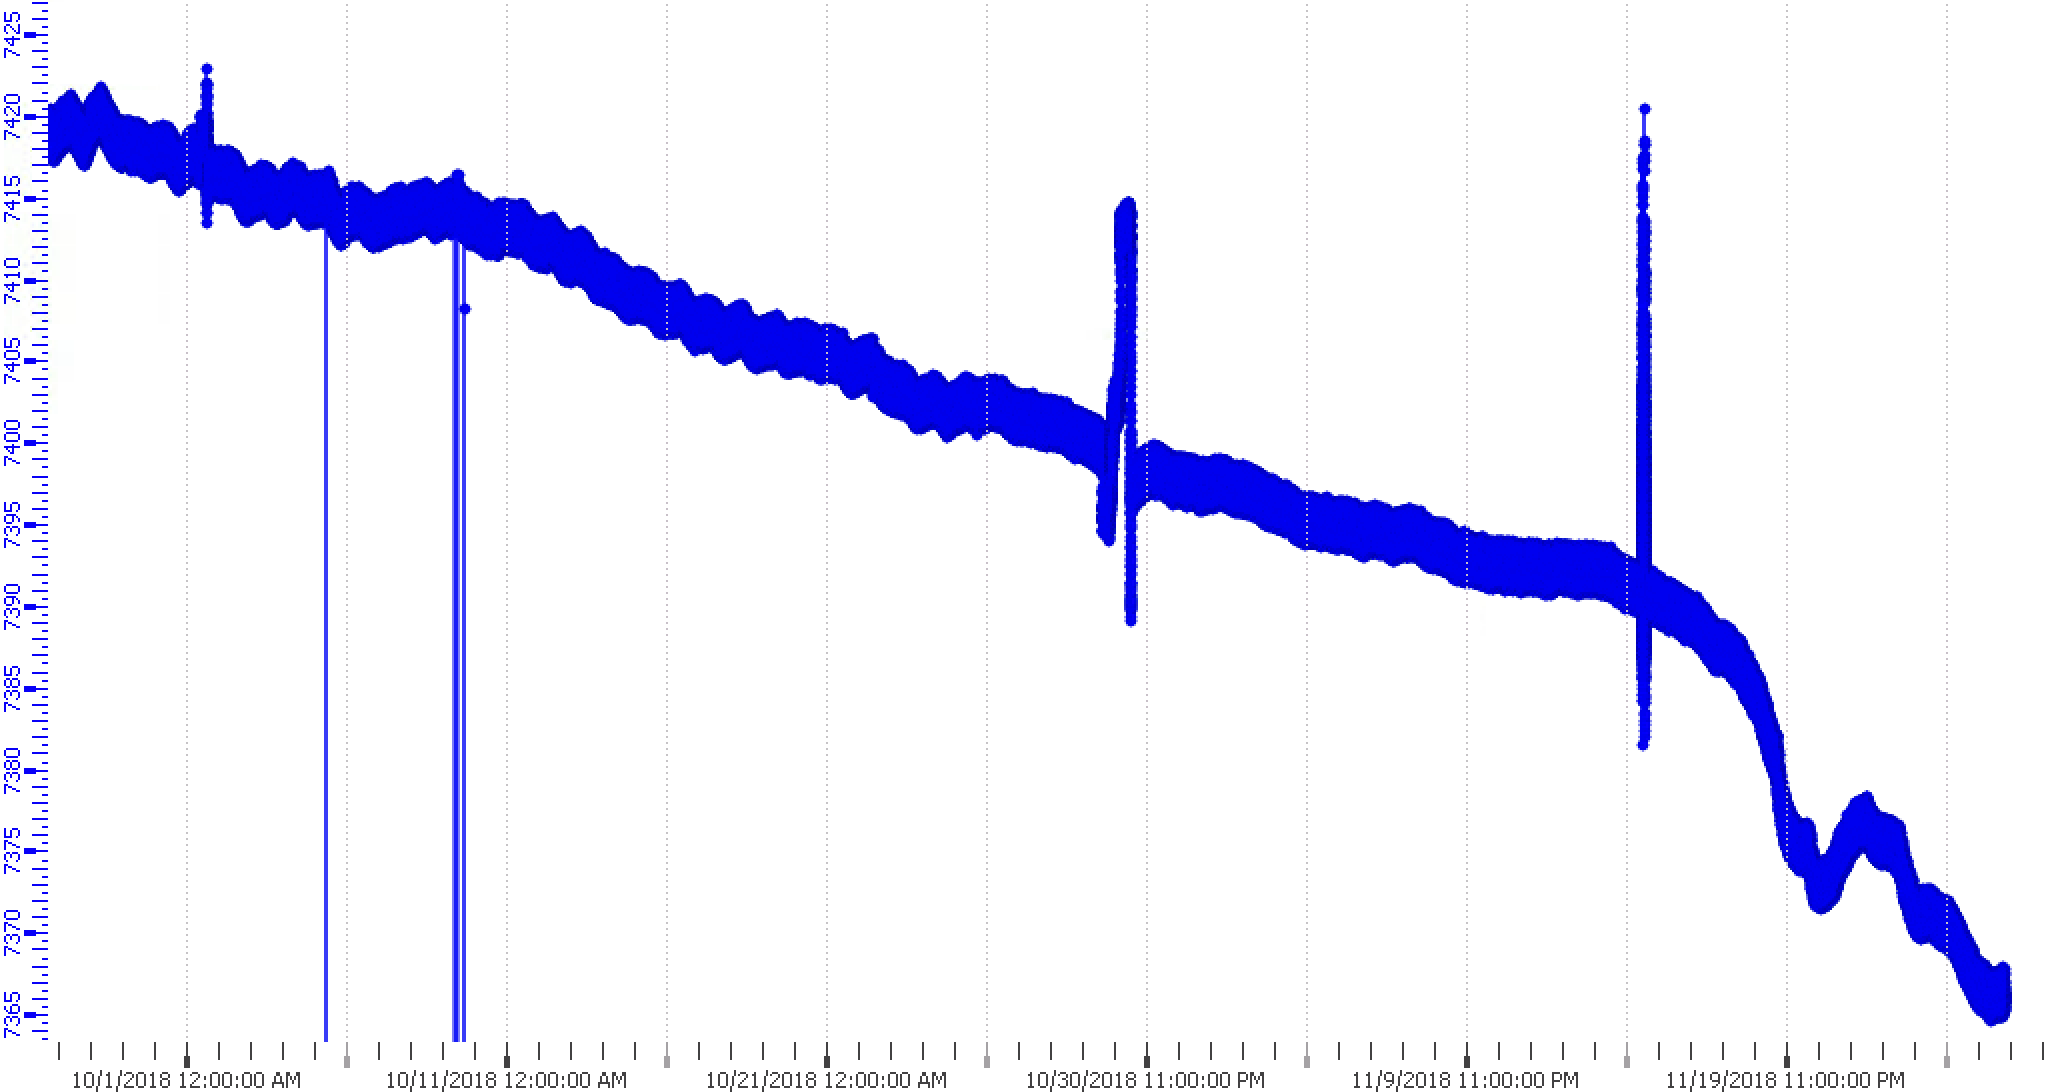
\includegraphics[width=0.4\textwidth]{cisc_level_cap.png}%
  \hspace*{1cm}
  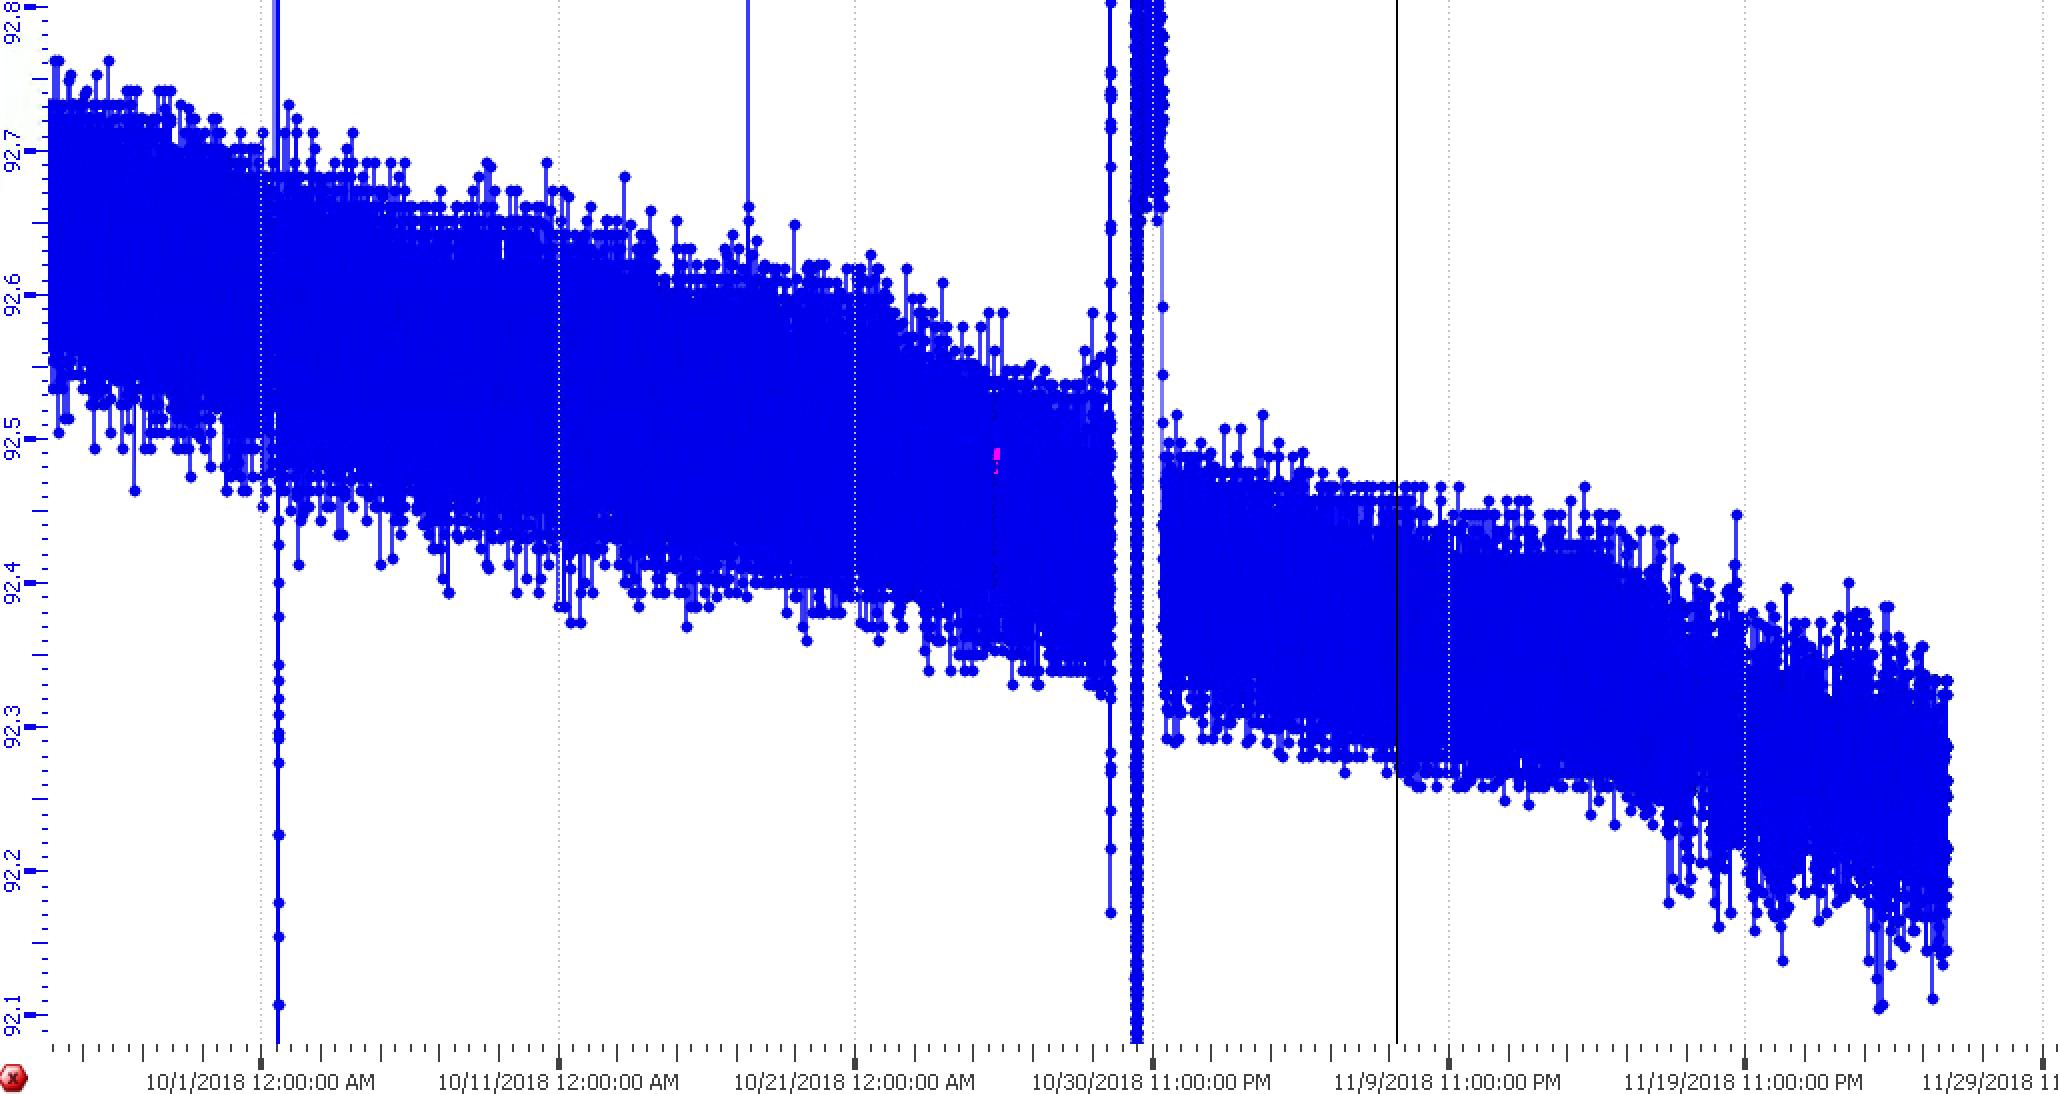
\includegraphics[width=0.4\textwidth]{cisc_level_diffp.png}%
\end{dunefigure}

%%%%%%%%%%%%%%%%%%% GAS ANALYZERS %%%%%%%%%%%%%%%%%%%%
\subsection{Gas Analyzers}
\label{sec:fdgen-slow-cryo-gas-anlyz}
% alan h

 Gas analyzers are commercially produced modules that measure trace quantities of specific gases contained within a stream of carrier gas. The carrier gas for DUNE is argon, and the trace gases of interest are oxygen ($\text{O}_2$), water ($\text{H}_2\text{O}$), and nitrogen ($\text{N}_2$). $\text{O}_2$ and $\text{H}_2\text{O}$ impact the electron lifetime in \dword{lar} and need to be kept to levels below \SI{0.1}{ppb} ($\text{O}_2$ equivalent) , while $\text{N}_2$ impacts the efficiency of scintillation light production at levels above \SI{1}{ppm}.
The argon is sampled from either the argon vapor in the ullage or from the \dword{lar} by the use of small diameter tubing run from the sampling point to the gas analyzer. Typically the tubing from the sampling points are connected to a switchyard valve assembly that is used to route the sample points to the desired gas analyzers (see figure~\ref{fig:GA-switchyard}).


\begin{dunefigure}[Photo of a Switchyard Valve Assembly]{fig:GA-switchyard}
  {A Gas Analyzer switchyard that routes sample points to the different gas analyzers.}
  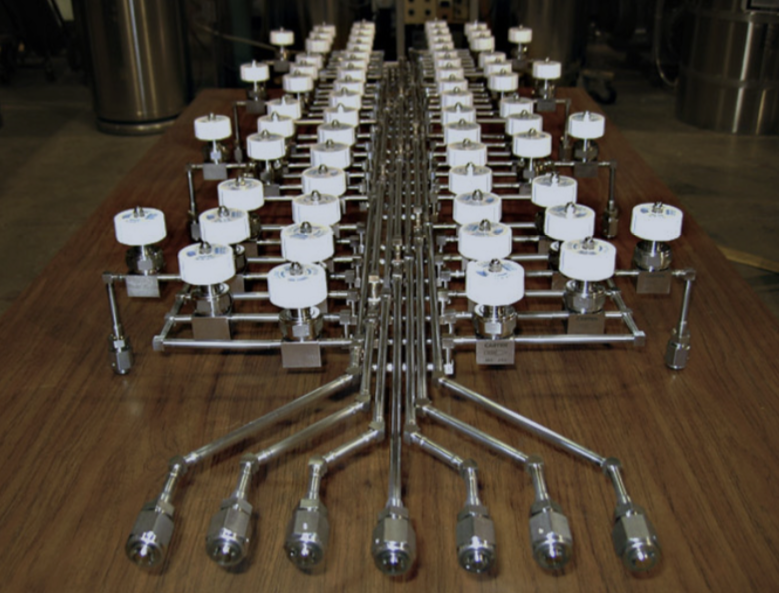
\includegraphics[width=0.9\textwidth]{cisc_GasAnalyzerSwitchyard.png}
\end{dunefigure}

The following list shows three examples of gas analyzer usage.


\begin{enumerate}
\item Following the elimination of the air atmosphere from the cryostat after detector installation to levels low enough to begin cooldown. This purge/gas recirculation process is detailed in Section~\ref{sec:fdgen-slow-cryo-install-ga}. Figure~\ref{fig:cisc_Phase1_purge_gas_recirculation} shows the evolution of the $\text{N}_2$, $\text{O}_2$, and $\text{H}_2\text{O}$ levels from gas analyzer data taken during the purge and recirculation stages of the DUNE \dword{35t} %Prototype P
phase 1 run.

\item Track trace $\text{O}_2$ and $\text{H}_2\text{O}$ contaminants from the $\>$tens of ppb to the hundreds of ppt. This is useful when other means of monitoring the impurity level (e.g., purity monitors, or \dshort{tpc} tracks) are not yet sensitive. Figure~\ref{fig:cisc_O2AnalyzerPrM2_HVRun1} shows an example plot of the $\text{O}_2$ level at the beginning of \dword{lar} purification from one of the later \num{35}\si{t} %Prototype 
\dword{hv} runs.

\item Monitor the tanker \dword{lar} deliveries purity during the cryostat-filling period. This allows tracking the impurity load on the filtration system and rejecting any deliveries that are out of specifications. Likely specifications for the delivered \dword{lar} are in the \SI{10}{ppm} range per contaminant.

\end{enumerate}

\begin{dunefigure}[Photo of a Switchyard Valve Assembly]{fig:cisc_Phase1_purge_gas_recirculation}
  {Plot of the O2, H2O, and N2 levels during the Piston Purge and Gas Recirculation stages of the 35 Ton Cryostat Phase 1 run}
  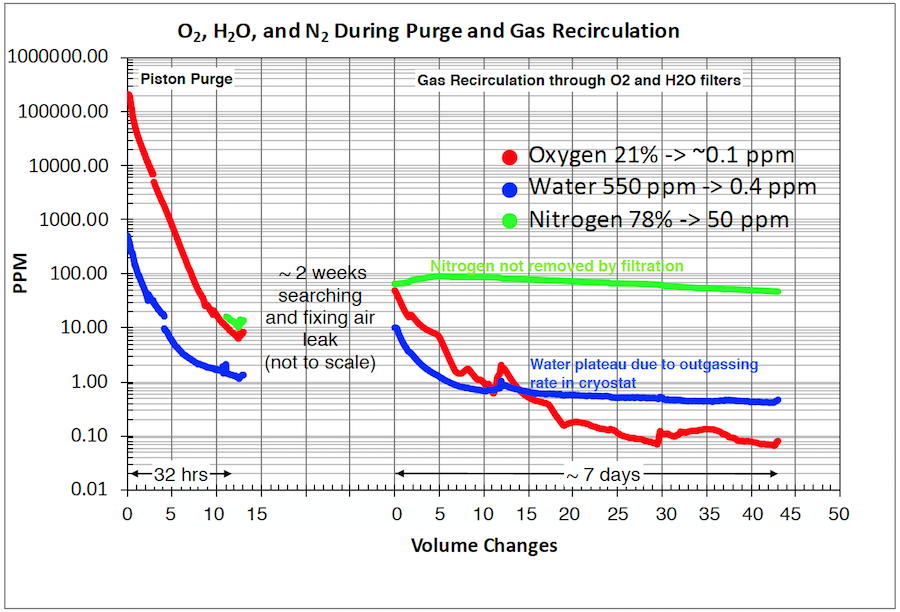
\includegraphics[width=0.7\textwidth]{cisc_Phase1_purge_gas_recirculation.png}
\end{dunefigure}

\begin{dunefigure}[Photo of a Switchyard Valve Assembly]{fig:cisc_O2AnalyzerPrM2_HVRun1}
  {O2 as measured by a precision O2 analyzer just after the 35T cryostat was filled with LAr, continuing with the LAr pump start and beginning of LAr recirculation through the filtration system. As the gas analyzer loses sensitivity, the purity monitor is able to pick up the impurity measurement. Note that the purity monitor is sensitive to both O2 and H2O impurities giving rise to its higher level of impurity.}
  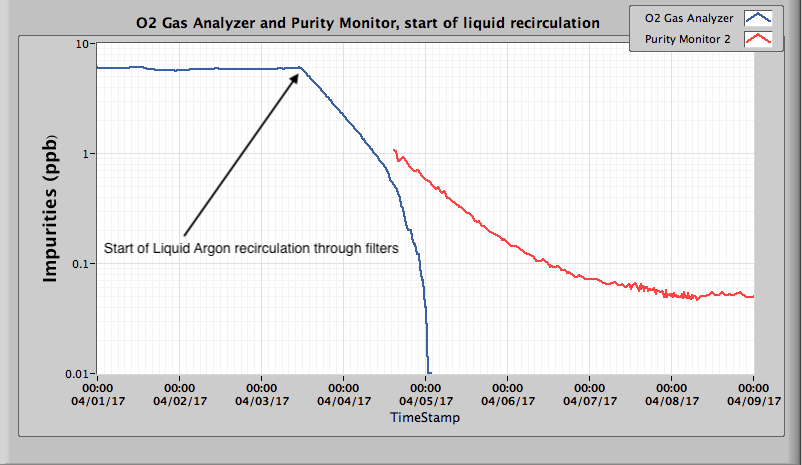
\includegraphics[width=0.7\textwidth]{cisc_O2AnalyzerPrM2_HVRun1.png}
\end{dunefigure}

As any one gas analyzer covers only one contaminant species and \numrange{3}{4} orders of magnitude of range, multiple units are needed both for the three contaminant gases and to cover the ranges that are seen between the cryostat closure to the beginning of \dshort{tpc} operations:
\SI{20}{\percent} to $\lesssim 100$~ppt for $\text{O}_2$,
\SI{80}{\percent} to $\lesssim 1$~ppm for $\text{N}_2$, and
$\sim \SI{1}{\percent}$ to $\lesssim 1$~ppb for $\text{H}_2\text{O}$.
Since the total cost of these analyzers exceeds $\SI{100}[\textdollar]{k}$, it is useful to be able to  sample more than a single location or cryostat with the same gas analyzers. At the same time, the tubing run lengths from the sample point should be as short as possible in order to keep the response of the gas analyzer timely. This puts some constraints on the sharing of devices since, for example, the argon deliveries are at the surface, perhaps necessitating a separate surface gas analyzer.

% \fixme{Do Gas Analyzers have ProtoDUNE design and results? Alan and Stephen say they weren't used as extensively at PDSP as at 35t, and "35t is also a prototype and has shown how gas analyzers can be used."}

%%%%%%%%%%%%%%%%%%%%%55 CAMERAS %%%%%%%%%%%%%%%%%%%%%%%%5
\subsection{Cameras}
% glenn, jim s, chuck
% same text in single and dual phase

Cameras provide direct visual information about the state of the
\dword{detmodule} during critical operations and when damage or unusual
conditions are suspected.  Cameras in the \dword{wa105} allowed spray from cool-down
nozzles to be seen and the level and state of the \lar to be
observed as it covered the \dword{crp} \cite{Murphy:20170516}.  A camera was
used in the Liquid Argon Purity Demonstrator
cryostat\cite{Adamowski:2014daa} to study \dword{hv} discharges in
\lar, and in EXO-100 during operation of a TPC
\cite{Delaquis:2013hva}.  Warm cameras viewing \lar from a distance
have been used to observe \dword{hv} discharges in \lar in
fine detail \cite{Auger:2015xlo}.  Cameras are commonly used during
calibration source deployment in many experiments (e.g., the
\kamland ultra-clean system \cite{Banks:2014hra}).

In DUNE, cameras are used to verify the stability, straightness,
and alignment of the hanging TPC structures during cool-down and
filling; to ensure that there is no bubbling near the \dwords{gp}
(\single) or \dwords{crp} (\dual); to inspect the
state of movable parts in the \dword{detmodule} (calibration devices, dynamic
thermometers) as needed; and to closely inspect parts of the TPC as
necessary following any seismic activity or other unanticipated
occurrence.  These functions are performed using a set of fixed
\textit{cold} cameras permanently mounted at fixed points in the cryostat
for use during filling and commissioning, and a movable, replaceable
\textit{warm} inspection camera that can be deployed through any free
instrumentation flange at any time throughout the life of the
experiment. 
% [GAHS: I commented out the table.] Table \ref{tab:fdgen-cameras-req} summarizes the requirements for the camera system.

Eleven cameras were deployed in \dword{pdsp} at the locations shown in Fig.~\ref{fig:pdsp-camera-locations}. They successfully provided views of the detector during filling and throughout the operation of the detector.

\begin{dunefigure}[Camera locations in \dword{pdsp}]{fig:pdsp-camera-locations}
  {A 3d view showing the locations of the 11 cameras in \dword{pdsp}.}
  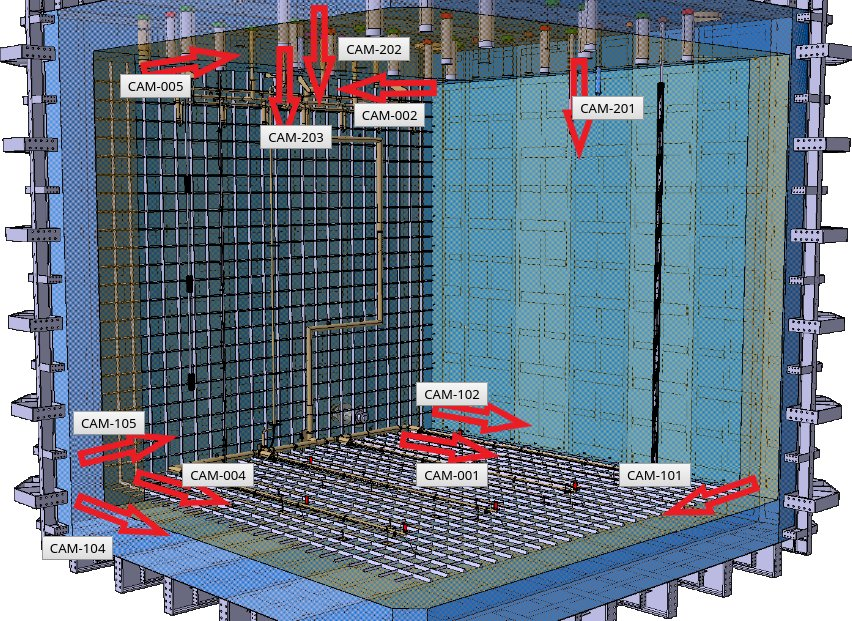
\includegraphics[width=0.6\textwidth]{pdsp-camera-locations-3d}%
\end{dunefigure}

The following sections describe the design considerations for the cold
and warm cameras and the associated lighting system and discuss the \dword{pdsp} camera systems' designs and performance.  
The same basic
designs may be used for both the single and dual phase detectors.

% GAHS: I commented out the table
% \begin{dunetable}
% [Camera system requirements]
% {p{0.45\linewidth}p{0.50\linewidth}}
% {tab:fdgen-cameras-req}
% {Camera system requirements}   
%  Requirement & Physics Requirement Driver \\ \toprowrule
%  \multicolumn{2}{l}{\bf General} \\ \specialrule{1.5pt}{1pt}{1pt}
%  No component may contaminate the \lar{}. & High \lar purity is required for TPC operation. \\ \colhline
%  No component may produce bubbles in the liquid argon if the \dword{hv} is on. & Bubbles increase risk of \dword{hv} discharge. \\ \colhline
%  No point in the camera system shall have a field greater than \SI{15}{kV/cm} when the drift field is at nominal voltage. & Fields must be well below \SI{30}{kV/cm} to avoid risk of \dword{hv} discharge.\\ \colhline
% The camera system shall not produce measurable noise in any detector system. & Low noise is required for TPC operation. \\ \colhline
%  Cameras provide the viewing functionality as agreed upon with the other subsystems for viewing, as documented in the ICDs with the individual systems. \\ \toprowrule
% \multicolumn{2}{l}{\bf Cold cameras}\\ \specialrule{1.5pt}{1pt}{1pt}
% Minimize heat dissipation when camera not in operation. & Do not generate bubbles when \dword{hv} is on. \\ \colhline
% Longevity must exceed \num{18} months. & Cameras must function throughout cryostat filling and detector commissioning. \\ \colhline
% Frame rate \(\geq\SI{10}{\per s}\). & Observe bubbling, waves, detritus, etc. \\ \toprowrule
% \multicolumn{2}{l}{\bf Inspection cameras}\\ \specialrule{1.5pt}{1pt}{1pt}
% Keep heat transfer to \lar low when in operation. & Do not generate bubbles, some use cases may require operation when \dword{hv} is on. \\ \colhline
% Deploy without exposing \lar to air. & Keep \lar free of N2 and other electronegative contaminants. \\ \colhline
% Camera enclosure must be replaceable. & Replace broken camera, or upgrade, throughout life of experiment. \\ \colhline
% {\bf Light emitting system} \\ \colhline
% No emission of wavelengths shorter than \(\SI{400}{nm}\) & Avoid damaging \dword{tpb} waveshifter. Note emitted wavelength shortens significantly with temperature. \\ \colhline
% Longevity must exceed \num{18} months. & Lighting for fixed cameras must function throughout cryostat filling and detector commissioning. \\ \colhline
% \end{dunetable}

%\fixme{Cameras intro: GAHS -- do we want to keep the separate, lower-level table of requirements for cameras?  I think we have to put key high-level requirements in the requirements table in the Requirements section, and drop this table. [dropped, but need to check for things to add to Requirements]}

%%%%%%%%%%%%%%%%%%%%%%%%%%%%%%%%%%%%%%%
\subsubsection{Cryogenic Cameras (Cold)}

The fixed cameras
monitor the following items during filling:
\begin{itemize}
\item Positions of corners of \dword{apa} or \dword{crp}, \dword{cpa} or cathode, \dwords{fc}, \dwords{gp} (\SI{1}{mm} resolution);
\item Relative straightness and alignment of \dword{apa}/\dword{crp}, \dword{cpa}/cathode, and \dword{fc} (\(<\sim\SI{1}{mm}\));
\item Relative position of profiles and endcaps (\SI{0.5}{mm} resolution);
\item State of \lar surface: e.g., the presence of bubbling or debris.
\end{itemize}


% GAHS: I commented out the past performance discussion because the PDSP cameras performed so well.
% There are published articles and unpublished presentations describing
% completely or partially successful operation of low-cost,
% off-the-shelf \dword{cmos} cameras in custom enclosures immersed in cryogens.
% (e.g., EXO-100: \cite{Delaquis:2013hva}; DUNE \dword{35t} test
% \cite{McConkey:2016spe}; \dword{wa105}: \cite{Murphy:20170516}.)  Generally
% it is reported that such cameras show poor performance and ultimately
% fail to function below some temperature of order \SIrange{150}{200}{K}, but some report that their cameras recover fully after
% being stored (not operated) at temperatures as low as \SI{77}{K} and
% then brought up to minimum operating temperature.

% However, as with photon sensors, experience has also shown that it is
% non-trivial to ensure reliable and reproducible mechanical and
% electrical integrity of such cameras in the cryogenic environment 
% (e.g., \cite{McConkey:2016spe} and
% \cite{Valencia-Rodriquez:20180130}).  Off-the-shelf cameras and camera
% components are generally only specified by the vendors and original
% manufacturers for operation down to \SI{-40}{\celsius} or \SI{-50}{\celsius}.
% In addition, many low-cost cameras use digital interfaces not intended
% for long distance deployment, such as USB (\(2\sim\SI{5}{m}\)) or CSI (circuit
% board scale), leading to signal degradation and noise problems.

One design for the DUNE fixed cameras uses an enclosure similar to
the successful EXO-100 design\cite{Delaquis:2013hva}, which was also
used successfully in the Liquid Argon Purity Demonstrator
and \dword{pdsp} (see Figure~\ref{fig:gen-fdgen-cameras-enclosure}). Cameras 101, 102, 104, and 105 shown in Fig.~\ref{fig:pdsp-camera-locations} use this enclosure.
A thermocouple in the enclosure allows temperature monitoring, and a heating element provides temperature control.  
SUB-D connectors are used at the cryostat flanges and the camera enclosure for signal, power, and control connections.
% The enclosure is connected to a stainless steel gas line to allow it to be flushed with argon gas at low enough pressure to prevent liquification, using the same design as the gas line for the beam plug tested in the \dword{35t} \dword{hv} test and in \dword{protodune}.  
%The camera transmits its video signal using either a composite video signal over shielded coax or Ethernet over optical fiber.  Most importantly, the DUNE \dword{cisc} consortium must work with vendors to design camera circuit boards that are robust and reliable in the cryogenic environment.

\begin{dunefigure}[A camera enclosure]{fig:gen-fdgen-cameras-enclosure}
  {Top left: a CAD exploded view of vacuum-tight camera enclosure suited for cryogenic applications from \cite{Delaquis:2013hva}.
    (1) quartz window, (2 and 7) copper gasket, (3 and 6) flanges, (4) indium wires, (5) body piece, (8) signal \fdth.
    Top right: two of the \dword{pdsp} cameras using stainless steel enclosure. 
    Bottom left: one of the \dword{pdsp} cameras using acrylic enclosure.
    Bottom right: a portion of an image taken with \dword{pdsp} camera 105 showing a purity monitor mounted outside of \dword{apa} on the beam left side. This photo was taken with \dword{pdsp} completely filled.
  }
  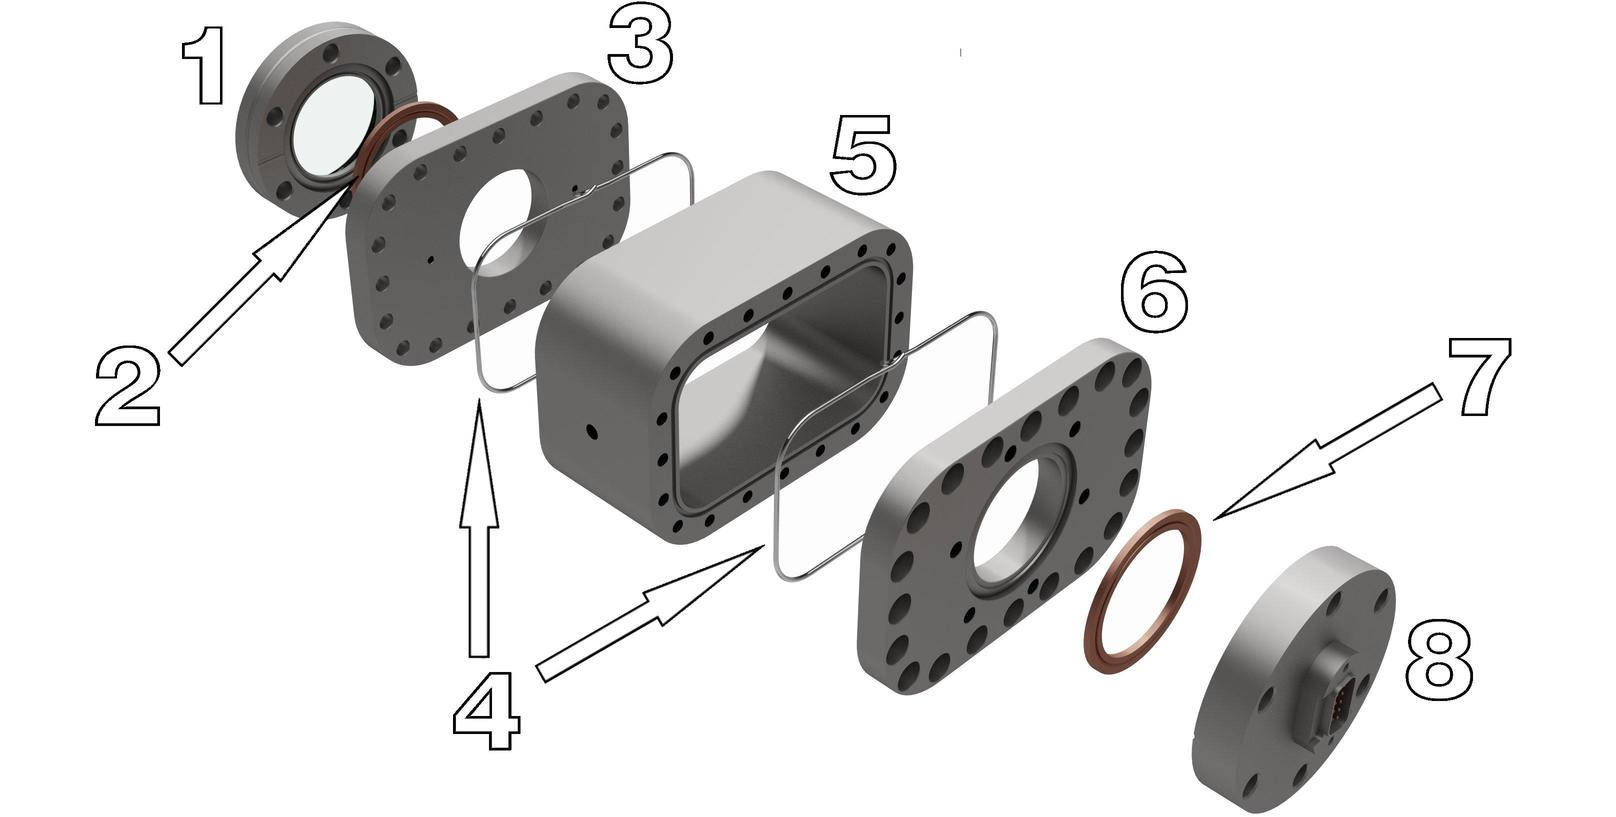
\includegraphics[width=0.4\textwidth]{exo100-camera-case}%
  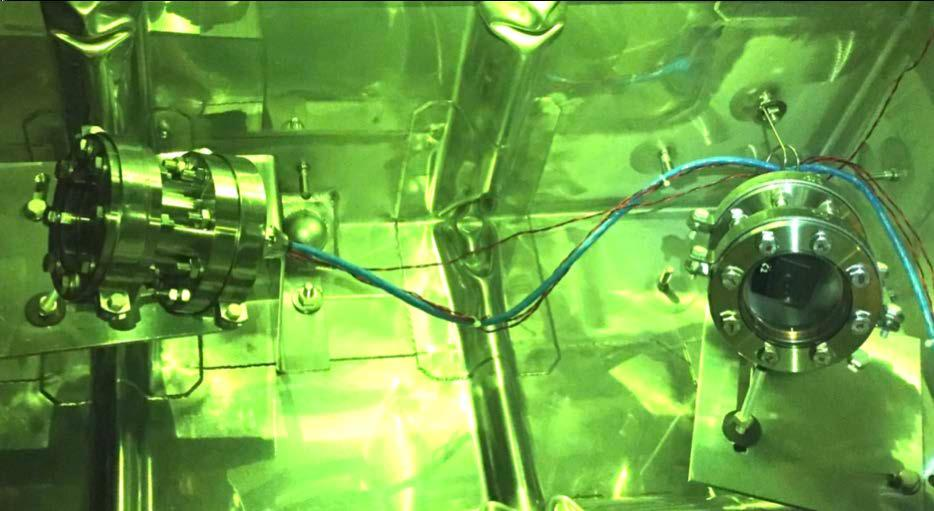
\includegraphics[width=0.4\textwidth]{edgar-cameras}\\
  \hfill 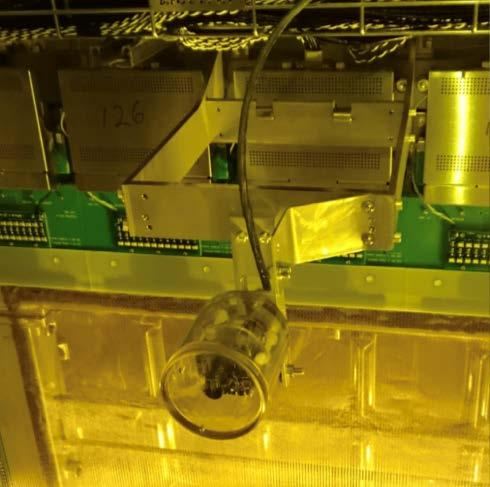
\includegraphics[width=0.22\textwidth]{bo-camera}%
  \hfill 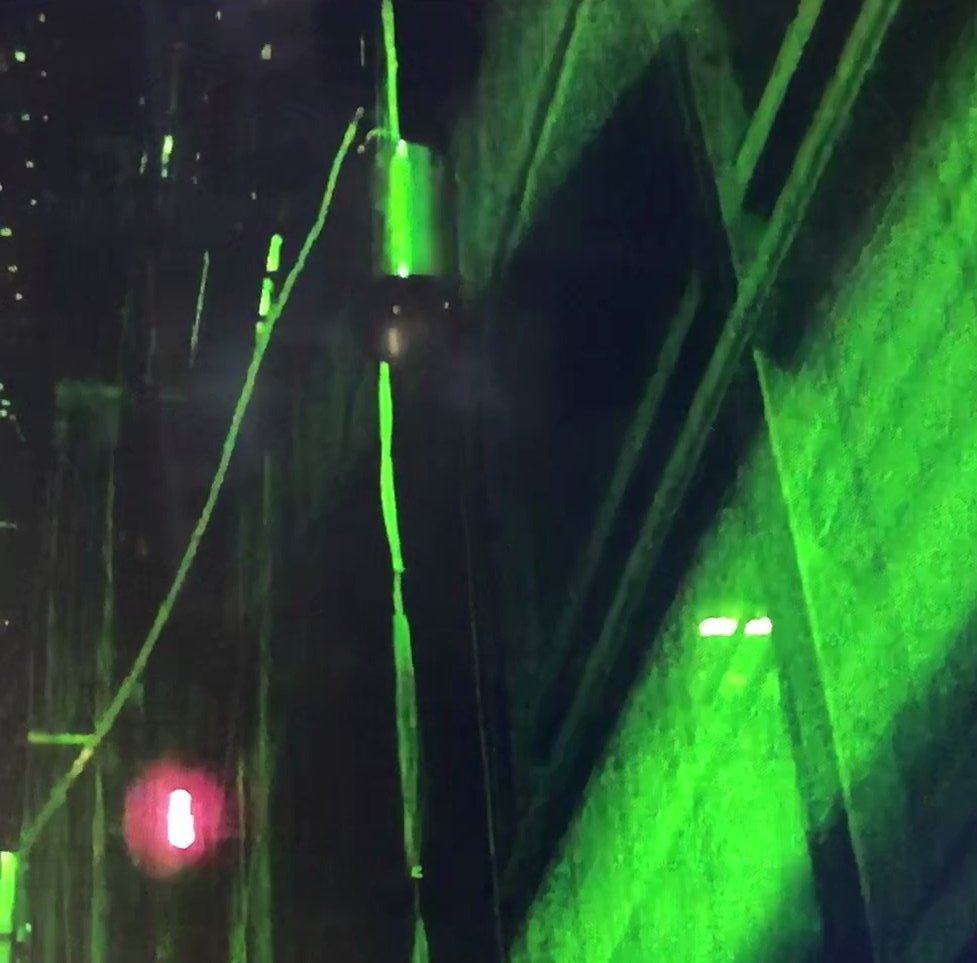
\includegraphics[width=0.22\textwidth]{camera-105-purmon-orig-rot-crop}%
  \hfill
\end{dunefigure}

An alternative design uses an acrylic enclosure.
This design was used successfully in \dword{pdsp} (see Figure~\ref{fig:gen-fdgen-cameras-enclosure}, bottom left). Cameras 001, 002, 004, and 005 shown in Fig.~\ref{fig:pdsp-camera-locations} use acrylic enclosures. 
All operated successfully, including those at the bottom of the cryostat.


%%%%%%%%%%%%%%%%%%%%%%%%%%%%%%%%%%%%%%%%%%%%%%%5
\subsubsection{Inspection Cameras (Warm)}

The inspection cameras are intended to be as versatile as possible.
However, the following locations have been identified as likely
to be of interest:
\begin{itemize}
\item Status of \dword{hv} \fdth and cup;
\item Status of \dword{fc} profiles, endcaps (\SI{0.5}{mm} resolution);
\item $y$-axis deployment of calibration sources;
\item Status of thermometers, especially dynamic thermometers;
\item \dword{hv} discharge, corona, or streamers on \dword{hv} \fdth, cup, or \dword{fc};
\item Relative straightness and alignment of \dword{apa}/\dword{crp}, \dword{cpa}/cathode, and \dword{fc} (\SI{1}{mm} resolution);
\item Gaps between \dword{cpa} frames (\SI{1}{mm} resolution);
\item Relative position of profiles and endcaps (\SI{0.5}{mm} resolution);
\item Sense wires at top of outer wire planes in \single \dword{apa} (\SI{0.5}{mm} resolution).
\end{itemize}

Unlike the fixed cameras, the inspection cameras need operate only as
long as inspection lasts, as the camera can be replaced in case of failure.  It
is also more practical to keep the cameras continuously \textit{warm}
(above \SI{-150}{\celsius}) during deployment; this offers %and therefore we willhave 
more options for commercial cameras, e.g., %.  For example, we could deploy 
the same model camera used successfully to observe discharges
in \lar from \SI{120}{cm} away \cite{Auger:2015xlo}.

\begin{dunefigure}[Inspection camera design]{fig:gen-fdgen-cameras-movable}
  {Left: An overview of the inspection camera design using a sealed deployment system opening directly into the cryostat. Right: A photo of the \dword{pdsp} warm inspection camera acrylic tube, immediately prior to installation; the acrylic tube is sealed with an acrylic dome at the bottom, and may be opened at the top.}
  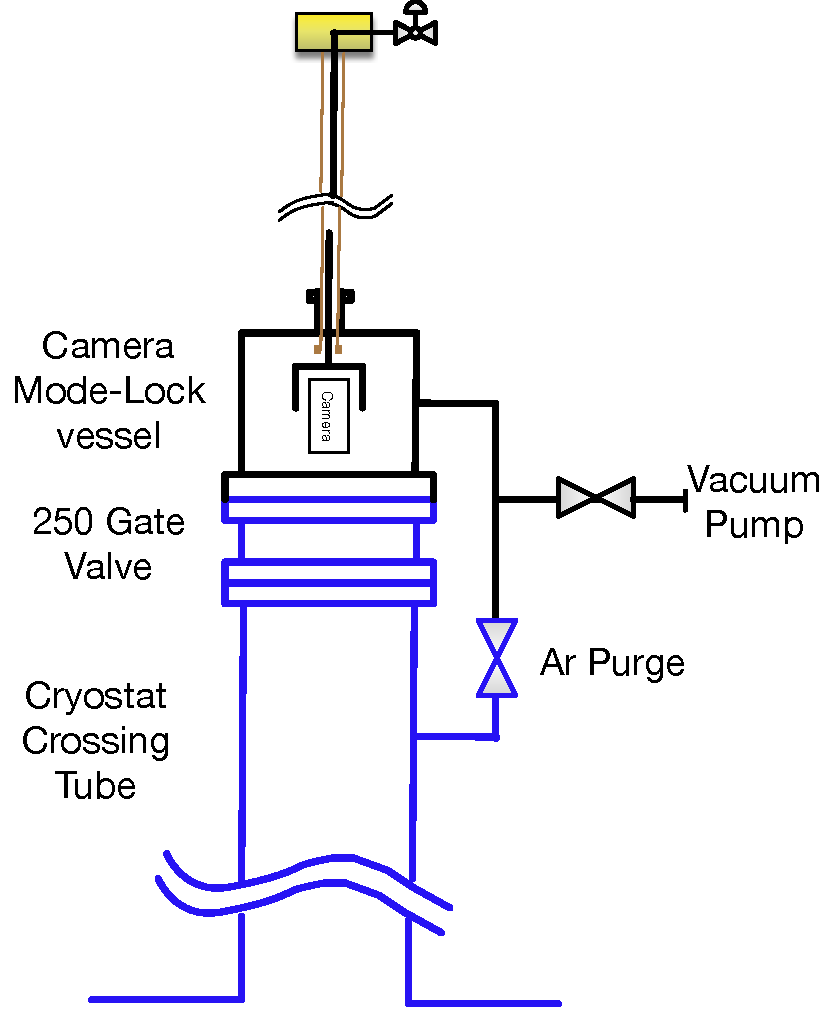
\includegraphics[height=0.3\textheight]{Camera-Sketch}%
  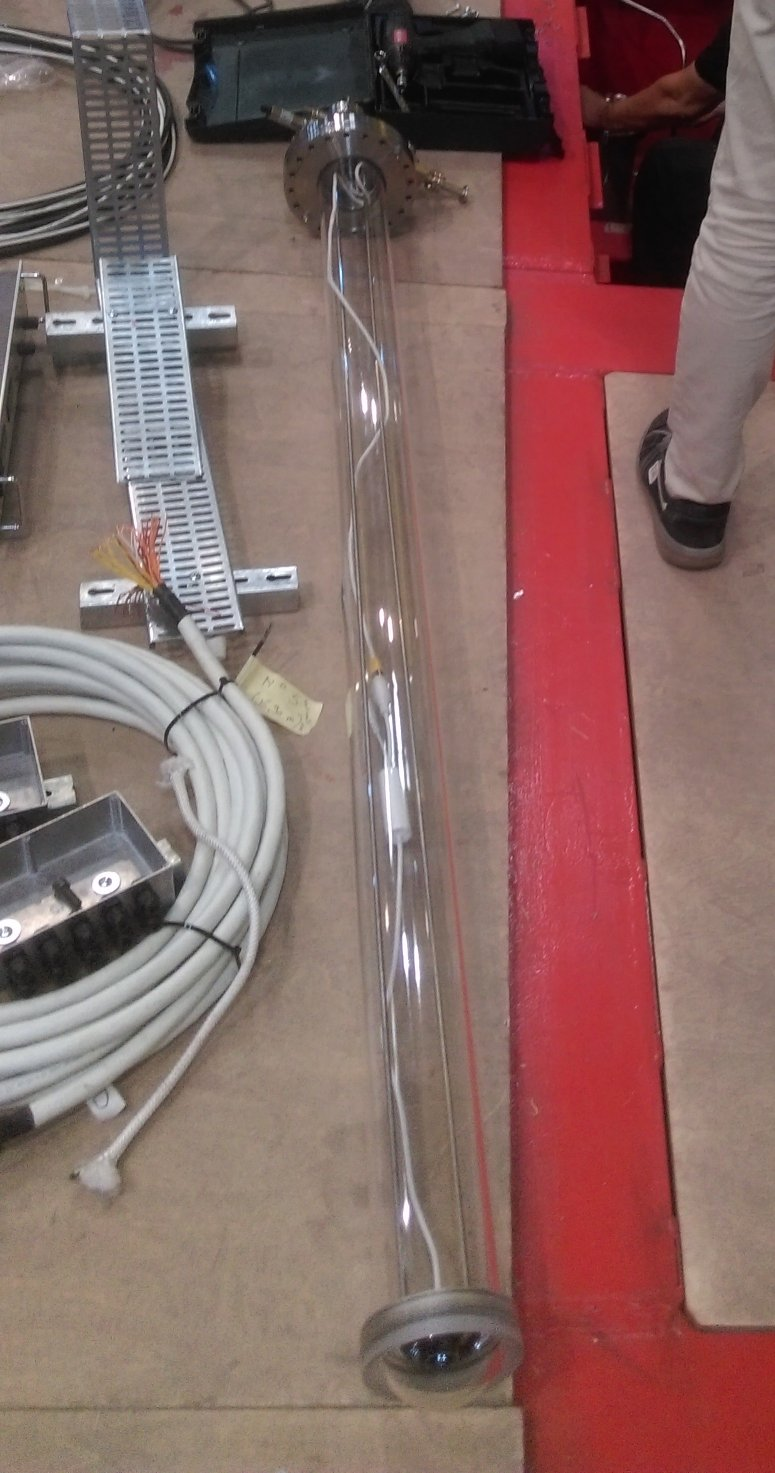
\includegraphics[height=0.3\textheight]{cisc-pdsp-camera-tube}%
\end{dunefigure}

The design for the inspection camera system employs the same basic
enclosure design as for cold cameras, but mounted on an insertable
fork using a design similar to the dynamic temperature probes. See
Figure~\ref{fig:gen-fdgen-cameras-movable}(left) and
Figure~\ref{fig:fd-slow-cryo-sensor-mount}.  The entire system is sealed to
avoid contamination with air. In order to avoid contamination, the
camera can only be deployed through a \fdth equipped with a gate
valve and a purging system, similar to that used for the vertical axis
calibration system at \kamland~\cite{Banks:2014hra}. The entire system
is  purged with pure argon gas before the gate valve is opened.

Motors above the flange allow rotation and vertical movement of the fork. 
 A chain drive system, with motor
mounted on the end of the fork, allows tilting of the camera assembly, 
creating a point-tilt mount with vertical motion capability.
Taking into account the room above the cryostat flanges and the
thickness of the cryostat insulation, a vertical range of motion of
\SI{1}{m} inside the cryostat is achievable.
% In the event that it
% becomes necessary to deploy a camera more deeply, we would have the
% option of building a a cable deployment system or a multi-pole
% deployment system similar to the KamLAND full-volume calibration
% system\cite{Busenitz:2009ac}, but this is not currently part of the
% baseline design.
The motors for rotation and vertical motion are located outside the sealed
volume, coupled mechanically using ferrofluidic seals, thus reducing
contamination risks and allowing for manual rotation of the vertical
drive in the event of a motor failure.  

An alternative design was demonstrated in \dword{pdsp}. In this design, the warm camera is contained inside a gas-tight acrylic tube inserted into the feedthrough. There is no need for a gate valve or a gas-tight rotatable stage, and the warm cameras can be removed for servicing or upgrade at any time. Fig.~\ref{fig:gen-fdgen-cameras-movable}(right) shows an acrylic tube enclosure and camera immediately before deployment. These acrylic tube enclosures for removable cameras were deployed at the positions marked 201, 202, and 203 in Fig.~\ref{fig:pdsp-camera-locations}; they operated successfully in \dword{pdsp}. Cameras with fisheye lenses were used in these tubes during initial operations; use of other cameras is planned during post-beam running.

Continuing prototyping and testing efforts are needed to finalize and validate these designs for DUNE, particularly with regard to longevity and pressure resistance.


%%%%%%%%%%%%%%%%%%%%%%%%%%%%%%%%%%%%%%%
\subsubsection{Light-emitting system}
%%% same text as dual-phase
The light-emitting system is based on \dwords{led} with the capability of illuminating the interior with selected
wavelengths (IR and visible) that are suitable for detection by the
cameras.  Performance criteria for the light-emission system are based
on the efficiency of detection with the cameras, in conjunction with
adding minimal heat to the cryostat. The use of very high-efficiency
\dwords{led}   
helps reduce heat generation; as an
example, one \SI{750}{nm} \dword{led} \cite{lumileds-DS144-pdf}
has a specification equivalent to
\SI{33}{\%} conversion of electrical input power to light.

% CEL: 1W electrical gives 425mW blue flux, power limit from SMD package thermal resistance of 8C/W to have max 1C increase at LED. CREE Xlamp XP-E model

While data on the performance of \dwords{led} at cryogenic temperatures is sparse,
some studies related to NASA projects~\cite{Carron:2017zzz} 
indicate that \dword{led} efficiency increases with reduced temperature,
and that the emitted wavelengths may change, particularly for blue \dwords{led}.
The wavelength changes cited would have no impact on illumination, however, since
in order  to avoid degradation of wavelength-shifting materials in the \dword{pds},
such short wavelength \dwords{led} would not be used.

\begin{dunefigure}[Example schematic for LED chain]{fig:cisc-LED}
  {Example schematic for LED chain, allowing failure tolerance and two LED illumination spectra.}
  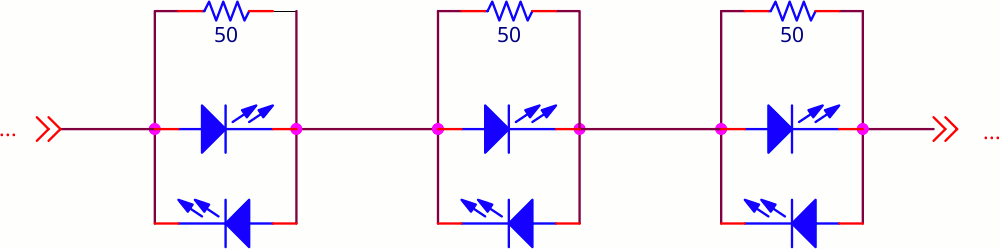
\includegraphics[width=0.6\textwidth]{cisc_led.png}
\end{dunefigure}

A \textit{chain} of \dwords{led} is connected in series and driven with a
constant-current circuit. It would be advantageous to pair each
\dword{led} in parallel with an opposite polarity \dword{led} and a resistor
(see Figure~\ref{fig:cisc-LED}).
This allows two different wavelengths of illumination with a single installed
chain (by changing the direction of the drive current) and 
continued use of an \dword{led} chain even if individual \dwords{led} fail.

The \dwords{led} should be placed as a \textit{ring light} around the outside of each
camera, pointing in the same direction as the lens, to 
illuminate the part of the \dword{detmodule} within the field of
view of the camera. Commercially available \dwords{led} can be obtained with
a range of angular spreads, and can be matched to the needs of the
cameras without additional optics.


%%%%%%%%%%%%%%%%%% CRYOGENIC TEST FACILITY %%%%%%%%%%%%%%%%%%%%
\subsection{Cryogenic Test Facility}
% same for SP and DP
% alan h

The Cryogenic Test Facility is intended to provide the access to a small (< \SI {1} {ton}) to intermediate (~\SI {5} {ton}) volumes of purified "TPC-grade" \dword{lar}. Hardware that needs this high purity liquid include any device intending to drift electrons for millisecond time periods. Not all devices need this high purity, but may need a relatively large volume to provide the needed prototyping environment. Of importance is a relatively fast turn-around time of approximately a week for short prototyping runs. 

\begin{dunefigure}[Photo of a Switchyard Valve Assembly]{fig:cisc_PAB_photo}
  {Photo of PAB Cryogenic Test Facility at FNAL.}
  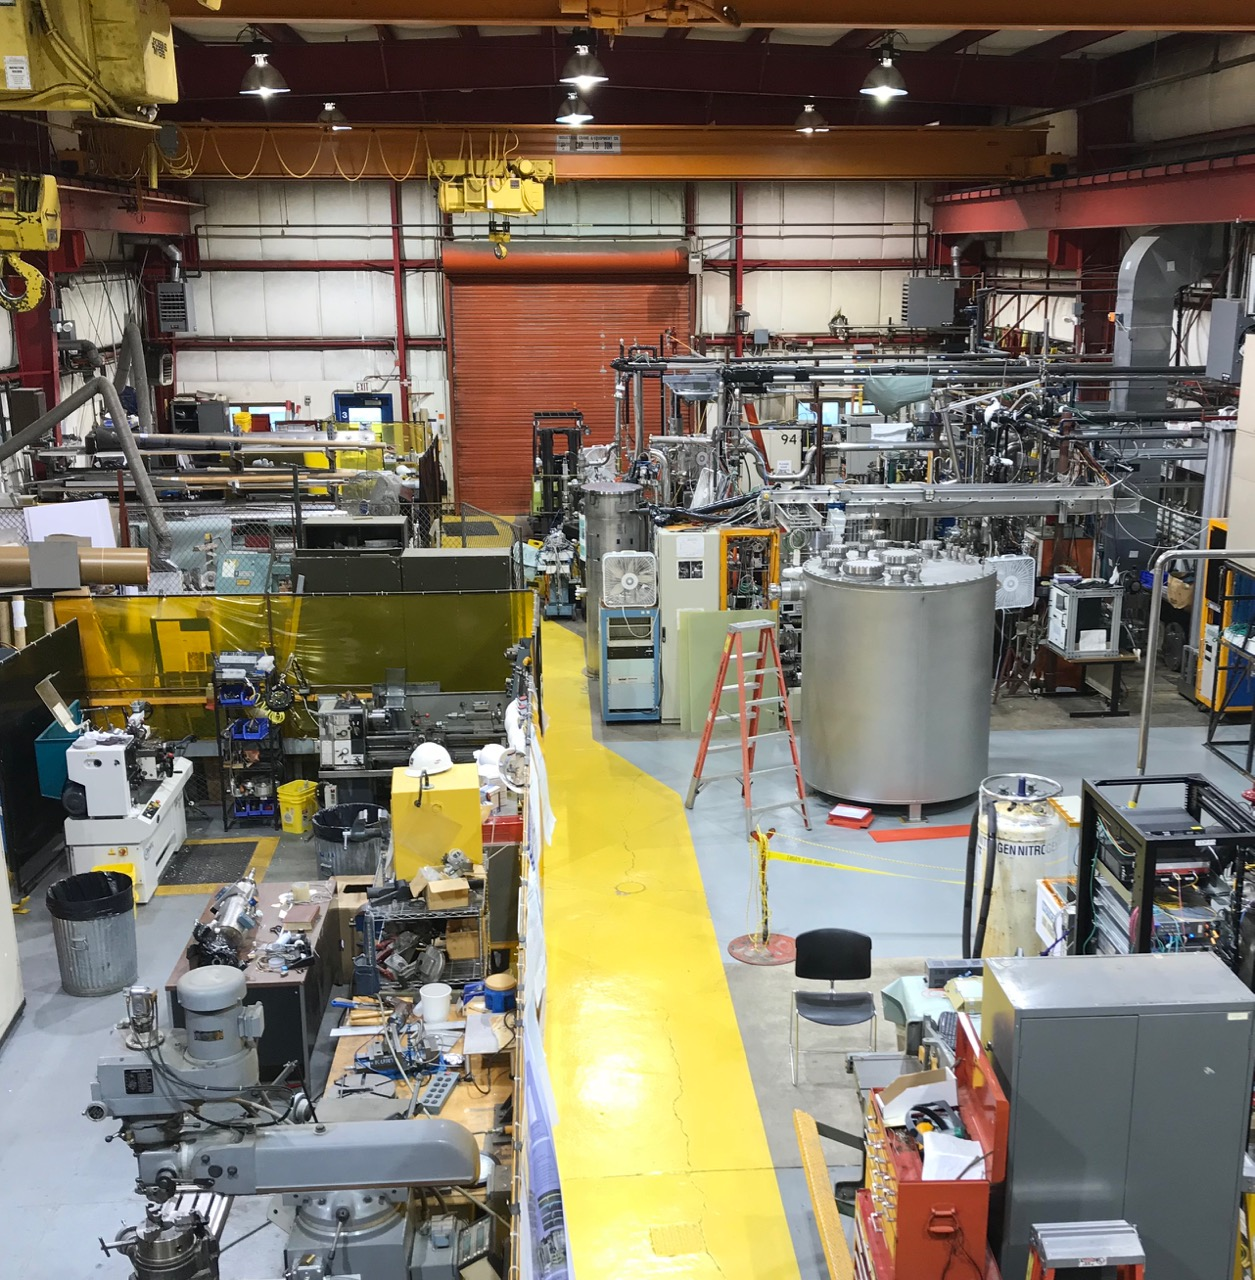
\includegraphics[width=0.9\textwidth]{cisc_PAB_photo.jpg}
\end{dunefigure}

Figure ~\ref{fig:cisc_PAB_photo} is a photo of the PAB facility at FNAL showing the ICEBERG \SI {3000} {liter} cryostat being readied for outfitting. This cryostat is intended to serve as a fast turn-around facility for the DUNE Cold Electronics Small TPC test facility. Also in the photo is a Tech Shop (left bottom) as well Tall Bo (\SI {450} {liter}), Blanche (\SI {500} {liter}) and Luke (\SI {250} {liter}) cryostats in the background. All these cryostats are available for outside use. In the recent past, Blanche has been used for \dword{hv} studies, Tall Bo for Photon Detector studies, and Luke has been utilized for the Material Test Stand work. These studies have contributed to the design and testing of ProtoDUNE \dword{sp} components.



%%%%%%%%
\section{Slow Controls}
% same for SP and DP

The slow controls system collects, archives, and displays data from
a broad variety of sources, and provides real time status, alarms and warnings for detector operators. Additionally, slow controls also provide control for some components of the detector systems such as \dword{hv} systems, \dword{tpc} electronics and photon detector system. Data is acquired via network interfaces.  Figure~\ref{fig:gen-slow-controls-diagram} shows the
connections between major parts of the slow controls system and other systems. Hardware, Infrastructure, and Software form the three main components of the slow controls system, each of which are described in this section.

\begin{dunefigure}[Slow Controls connections and data]{fig:gen-slow-controls-diagram}
{Typical Slow Controls system connections and data flow}
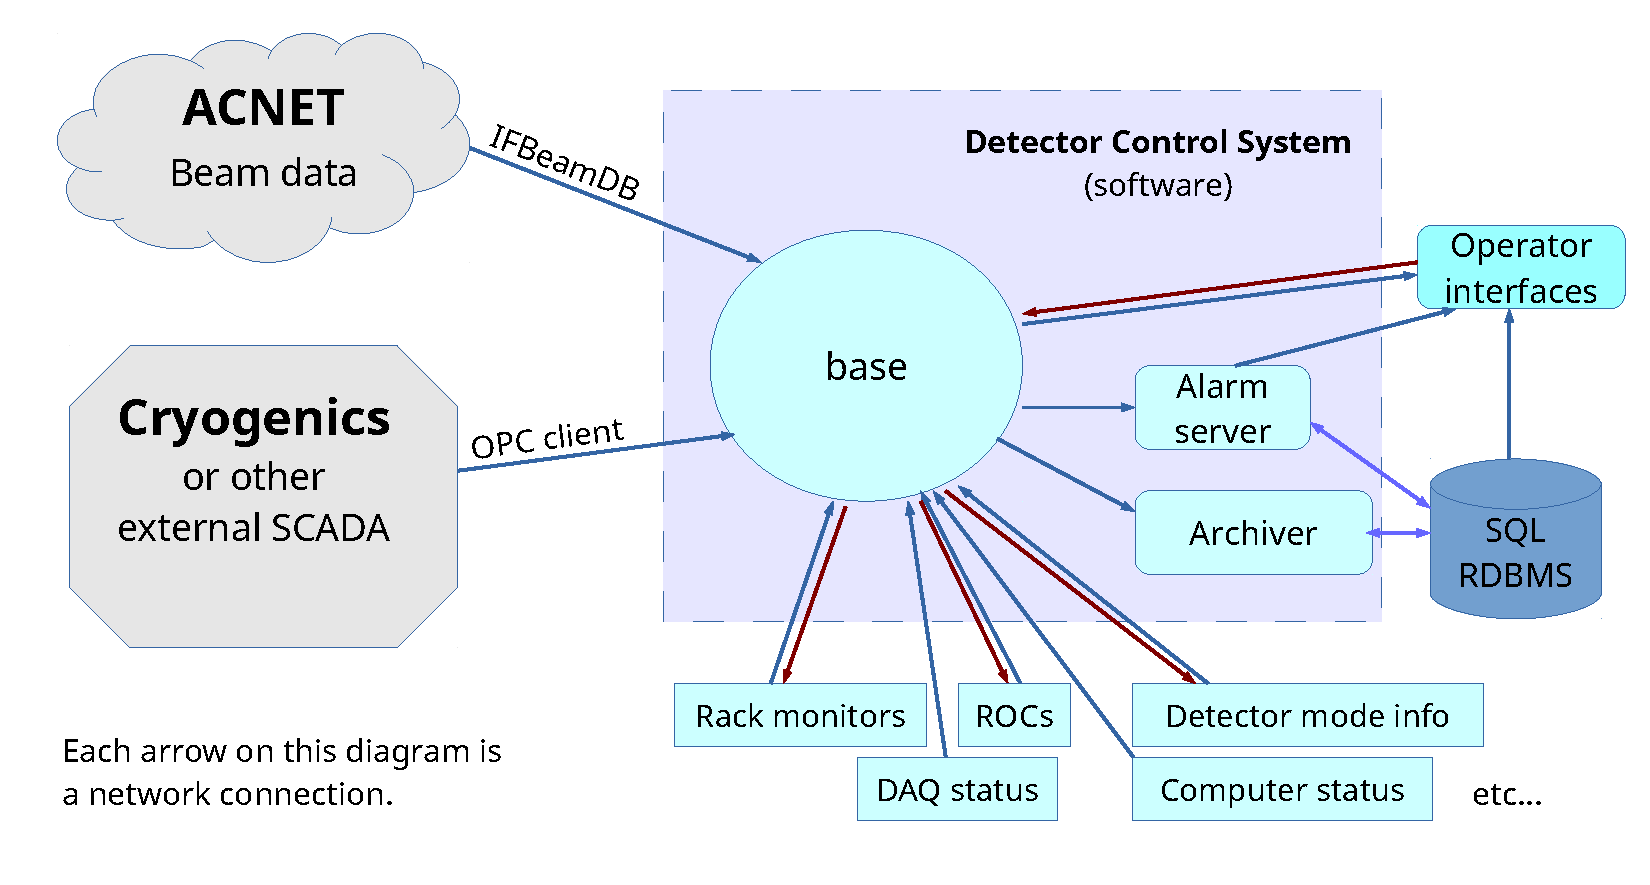
\includegraphics[width=0.7\textwidth]{cisc_slow-controls-diagram}
\end{dunefigure}

The \dword{pdsp} detector control system\cite{pdspdcs_proc} fully met the requirements for operating \dword{pdsp}. Section \ref{sec:cisc-slow-control-pdsp} provides a short description of the \dword{pdsp} slow controls and its performance.

%%%%%%%%%%%%%%%%%%%%%%%%%%%%%%%%%%%
 \subsection{Slow Controls Hardware}
\label{sec:fdgen-slow-cryo-hdwr}

A modest amount of dedicated hardware is envisioned for slow controls, largely for rack monitoring purposes. Additionally, slow controls will always require a small amount of dedicated network and
computing hardware as described below. Slow controls also relies on common
infrastructure, as described in
Section~\ref{sec:fdgen-slow-cryo-slow-infra}.

\subsubsection{Dedicated Monitoring Hardware}
Every rack (including those in the \dword{cuc}) is envisioned to have a dedicated hardware to monitor rack parameters such as rack protection system, rack fans, rack air temperatures, thermal interlocks with power supplies and any interlock bit status monitoring needed for the racks. For the racks in the \dword{cuc} server room, this functionality is built into the proposed water cooled racks as are currently being used at ProtoDUNE.  For the racks on the detector itself, the current plan is to design and install a custom-built 1U rack-mount enclosure containing a single-board computer to control and monitor various rack parameters. Such a system has been successfully used in MicroBooNE and the design is being improved for the Short-Baseline Near Detector (SBND) experiment, see Figure~\ref{fig:slow-controls-rack-box}. Other slow controls hardware is largely interfacing cables such as adapters for communication and debugging, or other specialized cables such as GPIB or from National Instruments. The cable requirements are yet to be determined in consultation with other groups once hardware choices for various systems are finalized.

\begin{dunefigure}[Rack monitoring box prototype being developed for the Short-Baseline Near Detector (SBND) experiment; based on the original design from MicroBooNE.]{fig:slow-controls-rack-box}
{Rack monitoring box prototype in development for the Short-Baseline Near Detector (SBND) experiment; based on the original design from MicroBooNE.}
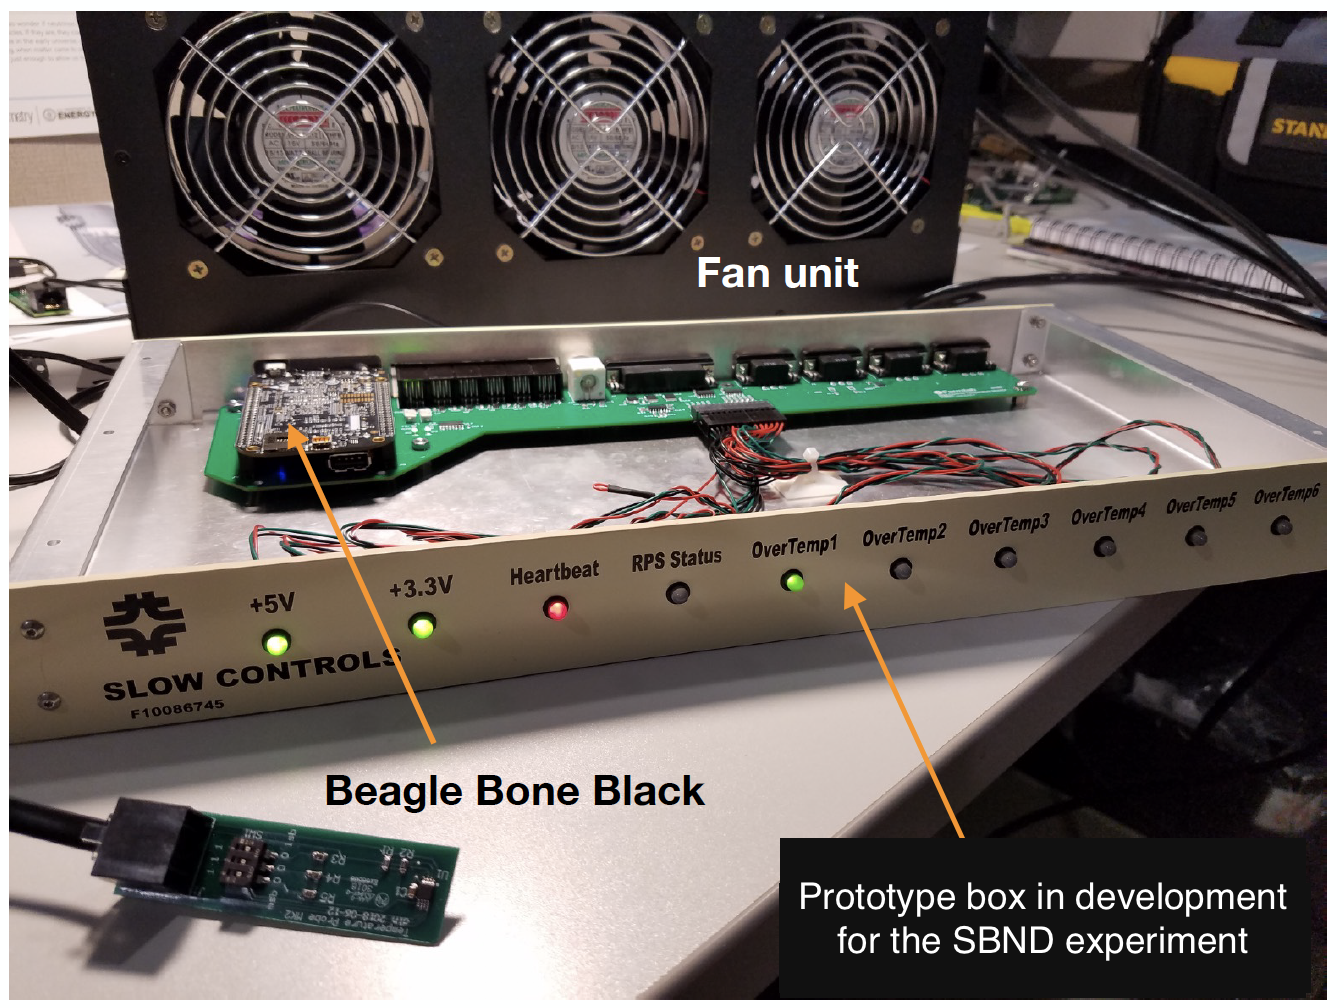
\includegraphics[width=0.6\textwidth]{cisc-slow-controls-rackbox.png}
\end{dunefigure}


% % % % Alec
\subsubsection{Slow Controls Network Hardware}
\label{sec:fdgen-slow-cryo-slow-network}
The slow controls data originates from the cryogenic instrumentation and from other systems as listed in Table~\ref{tab:gen-slow-quant}. This data is collected by software running on servers
(Section~\ref{sec:fdgen-slow-cryo-slow-compute})
housed in the underground data room in the \dword{cuc},
where data is archived in a central \dword{cisc} database.
The instrumentation data is transported over
conventional network hardware from any sensors located in the cryogenic
plant.  However, the readouts that are located in the racks on top the
cryostats must take care with grounding and noise.  Therefore, each
rack on the cryostat has a small network switch that sends
any network traffic from that rack to the \dword{cuc} via a fiber transponder.
This is the only network hardware specific to slow controls and will be provided by the lab's general computing infrastructure managed by the project \dword{tc} effort. The network infrastructure requirements are described in
Section~\ref{sec:fdgen-slow-cryo-slow-infra}.

% % % % Alec
\subsubsection{Slow Controls Computing Hardware}
\label{sec:fdgen-slow-cryo-slow-compute}
Two servers (a primary server and a replicated backup) suitable for the needed relational database discussed
in Section~\ref{sec:fdgen-slow-cryo-sw} are located in the \dword{cuc} data
room, with an additional
two servers to perform \dword{fe} monitoring interface services: for
example, assembling dynamic \dword{cisc} monitoring web pages from the adjacent
databases.  Another server to run back-end I/O will also be needed.  Any special purpose software, such as iFix used by the cryogenics experts, would
also run here. It is expected that one or two more servers will accommodate these programs.
% (The exact number of iFix machines will be determined based
% on input from the LBNF cryogenics experts.)
Replicating this setup on a per-module basis would allow for easier
commissioning and independent operation, accommodate different module
design (and the resulting differences in database tables), and ensure
sufficient capacity.  Including four sets of networking hardware, this
would fit tightly into one rack or very comfortably into two. The cost for servers and racks will be provided by the \dword{daq} consortium following the requirements from \dword{cisc}. 

% % % % Alec and Sowjanya
%% \subsubsection{Slow Controls Signal Processing Hardware}
%% Dropped because slow controls scope is defined not to include it.
%% (Signal processing should be within the scope of the hardware
%% generating the signal -- and so should digitization, for that matter.)
%%
%% N.B. The ``laundry list of Things to Be Monitored'' is in
%% \ref{sec:fdgen-slow-cryo-quant}



%%%%%%%%%%%%%%%%%%%%%%%%%%%%%%%%%%%
% Alec
\subsection{Slow Controls Infrastructure}
\label{sec:fdgen-slow-cryo-slow-infra}

The total number of slow controls quantities and the update rate are low enough
that the data rate will be in the tens of kilobytes per second range
(Section~\ref{sec:fdgen-slow-cryo-quant}), placing minimal requirements
on the local network infrastructure.
Network traffic out of \surf to \fnal will be primarily database calls
to the central \dword{cisc} database: either from monitoring applications, or from
database replication to the offline version of the \dword{cisc} database.  This
traffic is of a low enough bandwidth that the proposed general purpose
links both out of the mine and back to \fnal can accommodate it.

Up to two racks of space and appropriate power and cooling are
available in the \dshort{cuc}'s \dword{daq} server room for \dword{cisc} usage.
Somewhat less space than that is currently envisioned, as described in
\ref{sec:fdgen-slow-cryo-slow-compute}.

%%%%%%%%%%%%%%%%%%%%%%%%%%%%%%%%%%
% Sowjanya
\subsection{Slow Controls Software}
\label{sec:fdgen-slow-cryo-sw}
%\fixme{SG: does this need any updating based on presentations from Glenn/Alec at the Sept. Collaboration meeting? GAHS: I don't think so. PDSP DCS citation added. SG: okay, taking it out. I agree.}
% same for SP and DP

The slow controls software includes the following components in order 
to provide complete monitoring and control of detector subsystems:
%
\begin{itemize}
 \item{Control systems base} that performs input and output operations
  and defines processing logic, scan conditions, alarm conditions,
  archiving rate, etc.;
 \item{Alarm server} that monitors all channels and sends alarm
  messages to operators; 
 \item{Data archiver} that performs automatic sampling and storage of
  values for history tracking;
 \item{Integrated operator interface} that provides display panels for
  controls and monitoring.
\end{itemize}

An additional requirement for the software is the ability to indirectly
interface with external systems (e.g., cryogenics control
system) and databases (e.g., beam database) to export data into
slow controls process variables (or channels) for archiving and status
displays. This allows integrating displays and warnings into one
system for the experiment operators, and %to provide 
provides integrated
archiving for sampled data in the archived database. In this case, one
can imagine an input output controller (IOC) running on a central \dword{daq}
server provides soft channels for these data.
Figure~\ref{fig:gen-slow-controls-diagram} shows a typical workflow of a
slow controls system.

In terms of key features of the software, a highly evolved software is
needed that is designed for managing real-time data exchange, scalable
to hundreds of thousands of channels sampled at intervals of hours to seconds as needed. The software
should be well documented, supported, and known to be reliable. The base
software should also allow easy access of any channel by name. The
archiver software should allow data storage in an SQL database with
adjustable rates and thresholds such that one can easily retrieve data
for any channel by using channel name and time range. Among the key
features, the alarm server software should remember the state, support
arbitrary number of clients, and provide logic for delayed alarms and
acknowledging alarms. As part of the software, a standard naming
convention for channels is followed to aid dealing with large
number of channels and subsystems.

The \dword{pdsp} detector control system software \cite{pdspdcs_proc}
provides a prototype for the basis of the required \dword{fd} slow
controls software, and is referenced in the subsections below.

%%%%%%%%%%%%%%%%%%%%%%%%%%%%%%%%%%
% Ed T
\subsection{Slow Controls Quantities}
\label{sec:fdgen-slow-cryo-quant}

% starter text from Glenn

The final set of quantities to monitor will ultimately be determined
by the needs of the subsystems being monitored, as documented in
appropriate  interface control documents (ICDs), and continually revised based on operational
experience.  The total number of quantities to monitor has been roughly estimated by taking the total number of quantities monitored
in \dword{pdsp}\cite{pdspdcs_proc} --- a total of 7595 variables as of Nov. 19, 2018 --- and scaling by the detector length and the number of planes, giving a number around 200,000. %thousand. in the range of \numrange{140}{190} thousand. % let's keep just 1 digit of precision to be safe [glenn]
%\todo{Slow controls quantity estimate update --> \textbf{SG will estimate this number from ProtoDUNE based on info from Giovanna and update text.}}
Quantities are expected to update on average no faster than once per minute.
Transmitting a single update for each channel at that rate results in a few thousand updates per second, or a few tens of thousands of bytes per second. While this is not a significant load on the network given an efficient slow controls protocol, it would correspond to about 1~TB per year if every timestamp and value were stored.

The subsystems
to be monitored include the %detector 
cryogenic instrumentation
described in this chapter, the other detector systems, and relevant
infrastructure and external devices. Table \ref{tab:gen-slow-quant}
lists the kind of quantities expected from each system.

\begin{dunetable}
[Slow controls quantities]
{p{0.3\textwidth}p{0.6\textwidth}}
{tab:gen-slow-quant}
{Slow controls quantities}
System & Quantities \\ \toprowrule
\multicolumn{2}{l}{\bf Detector Cryogenic Instrumentation } \\ \specialrule{1.5pt}{1pt}{1pt}
Purity monitors & Anode and cathode charge, bias voltage and current, flash lamp status, calculated electron lifetime \\ \colhline
Thermometers & Temperature, position of dynamic thermometers \\ \colhline
Liquid level & Liquid level \\ \colhline
Gas analyzers & Purity level readings \\ \colhline
Cameras & Camera voltage and current draw, temperature, heater current and voltage, lighting current and voltage \\ \toprowrule
\multicolumn{2}{l}{\bf Other Detector Systems } \\ \specialrule{1.5pt}{1pt}{1pt}
Cryogenic internal piping & \fdth gas purge flow and temperature \\ \colhline
\dword{hv} systems & Drift \dword{hv} voltage, current; end-of-field cage current, bias; ground plane currents \\ \colhline
TPC electronics & Voltage and current to electronics \\ \colhline
\dword{pd} & Bias, current, electronics \\ \colhline
\dword{daq} & Warm electronics currents and voltages; run status; \dword{daq} buffer sizes, trigger rates, data rates, GPS status, etc.; computer and disk health status; other health metrics as defined by \dword{daq} group \\ \colhline
\dword{crp} / \dword{apa} & Bias voltages and currents \\ \toprowrule
\multicolumn{2}{l}{\bf Infrastructure and external systems } \\ \specialrule{1.5pt}{1pt}{1pt}
Cryogenics (external) & Status of pumps, flow rates, inlet and return temperature and pressure (via OPC or similar SCADA interface) \\ \colhline
Beam status & Protons on target, rate, target steering, beam pulse timing (via IFBeamDB) \\ \colhline
Near detector & Near detector run status (through common slow controls database) \\ \colhline
Racks power and status & Power Distribution Unit (PDU) current and voltage, air temperature, fan status if applicable, interlock status (fire, moisture, etc.) \\
Laser system & Overall status, laser power, temperature, operation modes\\
External neutron source system & Overall status, safety interlock status, power supply monitoring \\
External radioactive source system & Overall status\\
\end{dunetable}

%%%%%%%%%%%%%%%%%%%%%%%%%%%%%%%%%%
% Sowjanya and Anselmo
\subsection{Local Integration}
\label{sec:fdgen-slow-cryo-slow-loc-integ}

% This subsection is redundant with ``interfaces'', but there is a WBS
% section with the name ``Local integration'' that contains only interfaces,
% so keeping the subsection and adding some text saying what it is.

The local integration for the slow controls consists entirely of software
and network interfaces with systems outside of the scope of the \dword{detmodule}.
This includes the following:
\begin{itemize}
\item readings from the LBNF-managed external cryogenics systems, for status of pumps, flow rates, inlet and return temperature and pressure, which are implemented via OPC or a similar SCADA interfaces;
\item beam status, such as protons on target, rate, target steering, beam pulse timing, which are retrieved via IFBeamDB;
\item near detector status, which can be retrieved from a common slow controls database.
\end{itemize}

This integration occurs after both the slow controls and non-detector
systems are in place.  The LBNF-\dword{cisc} interface is managed by the
cryogenics systems working group in \dword{cisc} described in Section~\ref{sec:cisc-slow-controls-org}, which includes members from both \dword{cisc} and \dword{lbnf}. %\todo{Local integration section contains reference to WG previously described in IDR section on internal piping, but that section does not exist in TDR due to change of scope --> \textbf{SG? Please decide what to do}; SG: fixed it. I referenced to the organization and management section where this WG is described.}
The IFBeamDB interface for slow controls is already well established in MicroBooNE, NOvA, and other Fermilab experiments. An internal near-detector--\dword{fd} working group may be established in the future
to coordinate detector status exchange between near and far sites.

\subsection{Validation in ProtoDUNE}
\label{sec:cisc-slow-control-pdsp}

\begin{dunefigure}[Diagram of the \dword{pdsp} control system topology.]{fig:cisc-NP04-DCS-topology}
{Diagram of the \dword{pdsp} control system (NP04 DCS) topology, from \cite{pdspdcs_proc}.}
% Figure cannot be scaled down smaller than height=0.9\textheight,width=0.95\textwidth without making text unreadable. Even at this scale, the largest text on figure is 75% of the caption text font size. Authors of the NP04-DCS paper are making a new figure, just not ready for 1st TDR draft. [Glenn]
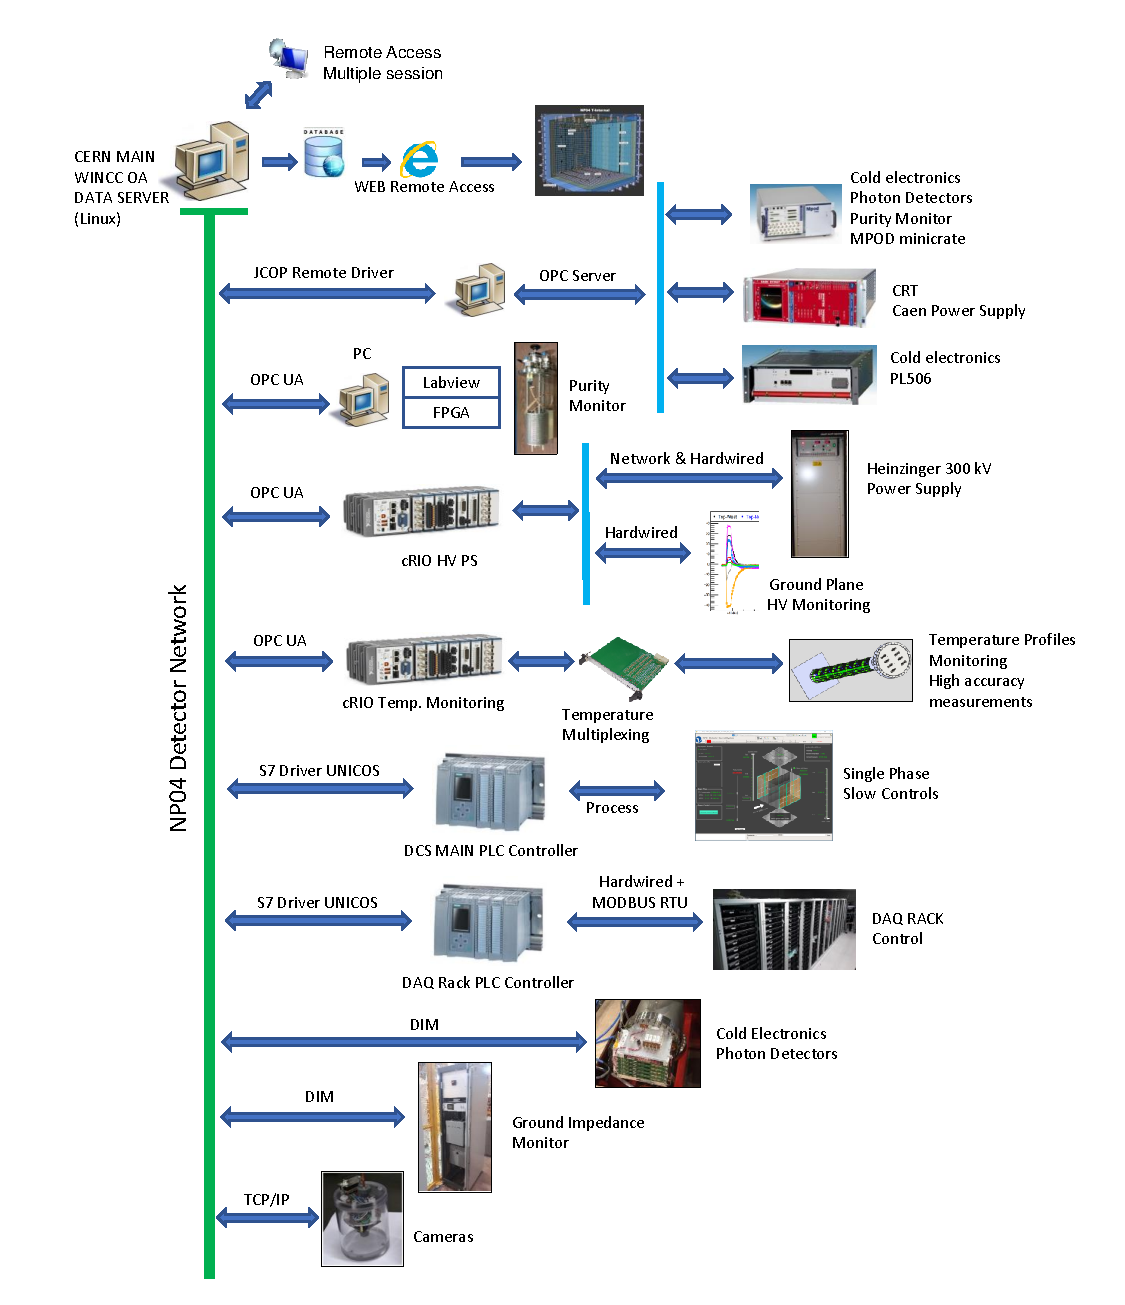
\includegraphics[height=0.9\textheight,width=0.95\textwidth,keepaspectratio]{NP04-DCS_arch_vert}
\end{dunefigure}

The \dword{pdsp} detector control system (also known as NP04-DCS) met
all requirements for operation starting in September, 2018, as
described in detail in \cite{pdspdcs_proc}.  Those requirements are
virtually identical to those of the \dword{fd}, with the exception of
total channel count. Of particular note, the NP04-DCS unified into a
single control system a heterogenous set of devices and data sources
through multiple protocols, as illustrated in
Fig.\ \ref{fig:cisc-NP04-DCS-topology}. In addition to those shown in
the figure, data was also acquired from external cryogenic and beam
systems.  The topology and data flow of the system matches the general
shape shown in Fig.\ \ref{fig:gen-slow-controls-diagram}. In NP04-DCS,
the unified control system base is WinCC OA\cite{winccoa}, a
commercial toolkit used extensively at CERN, with device interfaces
supported through multiple standardized interface protocols.

As noted in the software and quantities sections above, the DUNE ``slow'' control
system will be a massive data producer requiring a sizable database to store the history of values and allow for efficient data retrieval. Individually adjustable rates and thresholds for each channel are a key requirement for keeping this database manageable. The operation of the \dword{pdsp} provided not only a test of these features as implemented in the NP04 DCS, but also insight into reasonable values for these archiving parameters for each system.


%%%%%%%%
\section{Organization and Management}
\label{sec:cisc-slow-controls-org}

The organization of the CISC consortium is shown in
Fig.~\ref{fig:gen-slow-cryo-org}. The CISC consortium board is currently formed from institutional representatives from 19 institutes as shown in Table~\ref{tab:gen-slow-cryo-org}. The consortium leader acts as the spokesperson for the consortium and is responsible for the overall scientific program and management of the group. The technical leader of the consortium is responsible for the project management for the group. Currently five working groups are formed in the
consortium:
\begin{description}
 \item[Cryogenics Systems] gas analyzers \& liquid level
  monitors; \dword{cfd} simulations
 \item[Liquid Argon Instrumentation] purity monitors, thermometers, cameras and light emitting system, and instrumentation test facility; feedthroughs; \efield simulations; instrumentation precision studies; ProtoDUNE data analysis coordination and validation efforts
 \item [Slow Controls Base Software and Databases]  Base I/O software, alarms and archiving databases, and monitoring tools;
   variable naming convention and slow controls quantities
 \item [Slow Controls Detector System Interfaces] Signal processing software and hardware interfaces (e.g. power supplies); firmware; rack hardware and infrastructure   
 \item [Slow Controls External Interfaces] Interfaces with external detector systems (e.g. Cryogenics system, Beam, Facilities, \dword{daq}, near detector status)
\end{description}

\begin{dunefigure}[CISC consortium organization]{fig:gen-slow-cryo-org}
{CISC Consortium organizational chart}
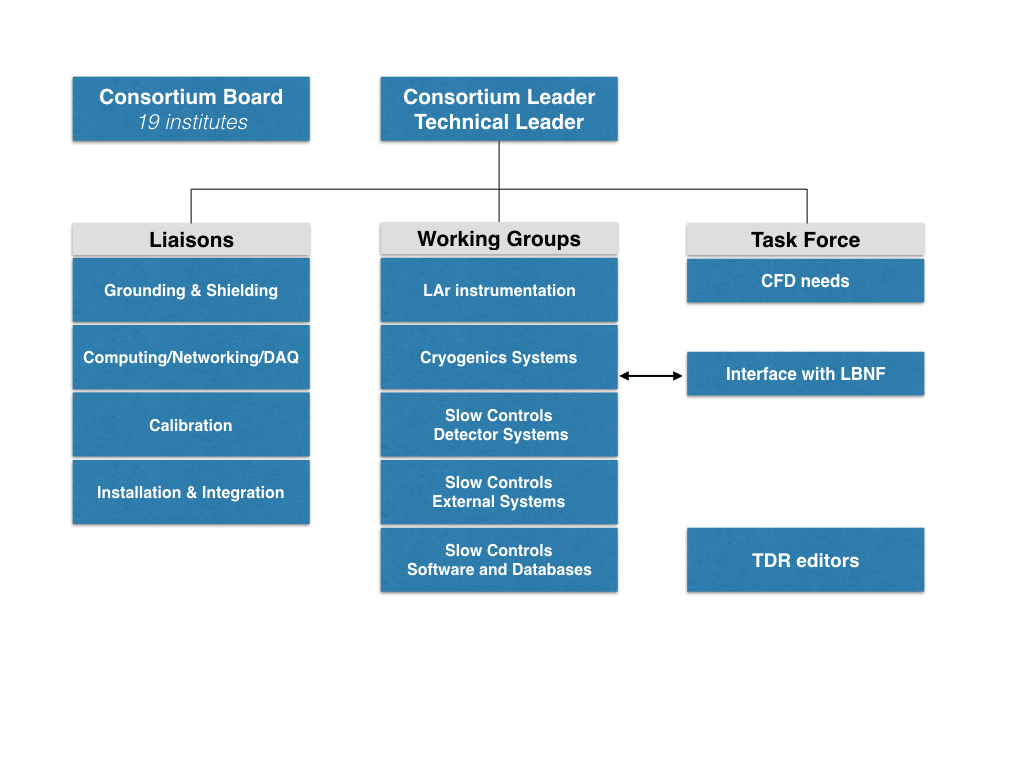
\includegraphics[width=0.7\textwidth]{cisc_org.png}
\end{dunefigure}

\begin{dunetable}
[CISC Consortium Institutions]
{p{0.43\textwidth}p{0.12\textwidth}p{0.22\textwidth}}
{tab:gen-slow-cryo-org}
{Current \dword{cisc} Consortium Board Members and their institutional affiliations}
Member Institute                         &  Country         &  Consortium Board Representative \\ \toprowrule
CIEMAT                                   &  Spain           &  Ines Gil Botella \\ \colhline
Instituto de Fisica Corpuscular (IFIC)          &  Spain           &  Anselmo Cervera \\ \colhline
University of Warwick                    &  UK  &  Gary Barker \\ \colhline
University College London (UCL)             &  UK  &  Mario Campanelli \\ \colhline
Argonne National Lab (ANL)                     &  USA             &  Jim Grudzinski  \\ \colhline
Brookhaven National Lab (BNL)                  &  USA             &  Jim Stewart \\ \colhline
University of California, Irvine (UCI)        &  USA             &  Jianming Bian \\ \colhline
Drexel University                        &  USA             &  Charles Lane \\ \colhline
Fermi National Accelerator Lab (FNAL)           &  USA             &  Alan Hahn \\ \colhline
University of Hawaii                     &  USA             &  Jelena Maricic \\ \colhline
University of Houston                    &  USA             &  Andrew Renshaw \\ \colhline
Idaho State University (ISU)                   &  USA             &  Ed Tatar \\ \colhline
Kansas State University (KSU)                  &  USA             &  Glenn Horton-Smith \\ \colhline
University of Minnesota, Duluth (UMD)         &  USA             &  Alec Habig \\ \colhline
Notre Dame University                    &  USA             &  John LoSecco \\ \colhline
South Dakota State University (SDSU)           &  USA             &  Stephen Gent \\ \colhline
University of Tennessee at Knoxville (UTK)     &  USA             &  Sowjanya Gollapinni \\ \colhline
Virginia Tech (VT)                            &	USA	            &  Camillo Mariani \\
\end{dunetable}

Additionally, since the CISC consortium broadly interfaces with other groups, liaisons have been identified for various roles as shown in Fig.~\ref{fig:gen-slow-cryo-org}. 
%\todo{names need to go away from the org chart figure --> \textbf{Anselmo will fix it.}}. 
A short-term task force was recently formed to understand the needs for cryogenic modeling for the consortium. A work plan for \dword{cfd} simulations for both ProtoDUNE and \dword{fd} was developed based on input from the task force. The \dword{tdr} editors are responsible for the overall editing and delivery of the \dword{tdr} document to the collaboration. Currently members from new institutes are added to the consortium based on consensus from the consortium board members following an expression of interest petition from the new institute.

\subsection{Institutional Responsibilities}

The slow controls and cryogenic instrumentation will be a joint effort for single and dual phase. A single slow controls system will be implemented to serve both \dword{dp} and \dword{sp} detectors.

Design and installation of cryogenic systems (gas analyzers, liquid level monitoring) will be coordinated with \dword{lbnf}, with the consortium providing resources and effort, and expertise provided by \dword{lbnf}. ProtoDUNE designs for liquid argon instrumentation (purity monitors, thermometers, cameras, test facility) will be the basis for \dword{fd} designs. Design validation, testing, calibration, and performance will be evaluated through ProtoDUNE data.

Following the conceptual funding model envisioned for the consortium, various responsibilities have been distributed across institutions within the consortium. At this stage of the project, these should be considered as ``aspirational'' responsibilities until firm funding decisions are made. Table~\ref{tab:cisc-inst-resp} shows the current institutional responsibilities for primary \dword{cisc} sub-systems. Only lead institutes are listed in the table for a given effort. For physics and simulations studies, and validation efforts with ProtoDUNE, number of institutes are involved. A detailed list of tasks and institutional responsibilities are presented in \dword{dune} DocDB 5609.

\begin{dunetable}
[Institutional Responsibilities in the \dword{cisc} consortium ]
{p{0.4\textwidth}p{0.45\textwidth}}
{tab:cisc-inst-resp}
{Institutional Responsibilities in the \dword{cisc} consortium}
CISC Sub-system     &  Institutional Responsibility \\ \toprowrule
Purity Monitors          &  UCI, Houston \\ \colhline
Static T-Gradient Monitors     &  IFIC \\ \colhline
Dynamic T-Gradient Monitors & Hawaii \\ \colhline
Individual Sensors & IFIC \\ \colhline
Readout System for Thermometers & IFIC, Hawaii, CIEMAT \\ \colhline
Cold Cameras & KSU, BNL \\ \colhline
Warm Cameras & KSU, BNL \\ \colhline
Light-emitting System (for cameras) & Drexel \\ \colhline
Gas Analyzers & FNAL, \dword{lbnf} \\ \colhline
Liquid Level Monitors & \dword{lbnf}, Notre Dame \\ \colhline
Instrumentation Test Facility & FNAL, ANL \\ \colhline
\dword{cfd} Simulations & SDSU, ANL \\ \colhline
Other Simulation \& Validation Studies & Number of Institutes \\ \colhline
Slow Controls Hardware & UMD, UTK, Drexel\\ \colhline
Slow Controls Infrastructure & UMD, UTK\\ \colhline
Slow Controls Base Software & KSU, UTK, Drexel, Warwick, UCL, ANL, IFIC\\ \colhline 
Slow Controls Signal Processing & Number of institutes \\
\end{dunetable}

\subsection{Cost and Labor}

Table \ref{tab:cisc-cost} shows the current cost estimates for the different \dword{cisc} subsystems. Table also shows the quantity associated with each subsystem and a brief description of what is included in the cost estimate. The cost estimates only include costs associated with materials and supplies (M\&S) and packing and shipping, and do do not include labor and travel costs. Since labor costs depend on the personnel category (e.g. faculty, student, technician, post-doc, engineer),and vary with regions and institutions, they are quantified in terms of labor hours needed to fulfill a given task. An estimate of labor hours for each subsystem is shown in Table~\ref{tab:cisc-labor}. A total of 95,010 labor hours are estimated for all \dword{cisc} tasks. 

\begin{dunetable}
[CISC Cost]
{p{0.3\textwidth}p{0.08\textwidth}p{0.1\textwidth}p{0.45\textwidth}}
{tab:cisc-cost}
{Cost estimates of the different CISC subsystems. All cost estimates include pacing and shipping costs.}
System                         & Quantity & Cost & Description  \\ \toprowrule
Purity Monitors                & 10 & \$309,400 & Includes material cost, PC, flanges, mounting structure  \\ \colhline
Static T-gradient monitors     & 6 & \$88,340 & Includes cables, sensors and connectors, support structure, flanges \\ \colhline
Precision Individual temperature sensors & 130 & \$51,512 & Includes cables, sensors and connectors, support structure, flanges \\ \colhline
Standard Individual temperature sensors & 35 & \$12,615 & Includes cables, sensors and connectors, support structure, flanges \\ \colhline
Dynamic T-gradient monitors    & 2 & \$108,060 & Includes cables, sensors, motor drive, flanges, sensor holders \\ \colhline
Warm Cameras                   & 3 & \$294,775 & Includes material cost, computer, argon purge \& pressurization system, prototyping \& testing  \\ \colhline
Cold Cameras                   & 12 & \$38,300  & Includes material cost, computer, minor jigs \& test boards \\ \colhline
Light system                   & 15 & \$4,900 & Cost of illuminator and light driver module    \\ \colhline
Gas analyzers                  & 1 & \$222,360 & Cost of gas analyzers and piping \& routing panel  \\ \colhline
Capacitive Level meters        & 4 & \$19,018  & Cost of level meters and flanges   \\ \colhline
Cryogenics Test Facility       & 1 & \$62,000  & Material cost mainly includes liquid argon costs for years 1 to 5 and minor fixturing costs  \\ \colhline
Slow Controls Hardware         & - & \$78,970  & Cost of 6 servers, 0.5 rack, 126 rack monitoring boxes, and cables   \\ \colhline
Slow Controls Software         & - & \$1,500 & Includes cost of a laptop    \\ \colhline
\textbf{Total Cost}          &       & \textbf{\$1,291,750}& \\
\end{dunetable}

\begin{dunetable}
[CISC labor]
{p{0.25\textwidth}p{0.15\textwidth}p{0.1\textwidth}p{0.08\textwidth}p{0.08\textwidth}p{0.1\textwidth}p{0.08\textwidth}}
{tab:cisc-labor}
{Estimate of labor hours for each category of personnel for different CISC subsystems. In the case of slow controls software, the 884 technician hours contains 442 hours of Information Technology professional and 442 hours of scientific computing professional.}
System  & Faculty/Scientist & Post-doc & Student & Engineer & Technician  &  \textbf{Total}\\ \toprowrule
& (hours) & (hours)& (hours)& (hours)& (hours)& (hours)\\ \toprowrule
Purity Monitors & 5304& 5304& 5304& -& 1326 & \textbf{17238} \\ \colhline
Static T-gradient monitors & 3536& 1768& 2652&  442& 884& \textbf{9282} \\ \colhline
Individual temperature sensors & 3536& 1768& 2652&  442& 884& \textbf{9282} \\ \colhline
Dynamic T-gradient monitors & 3536& 3536& 3536&  354& 884& \textbf{11846} \\ \colhline
Warm Cameras & 1768& 1768& 1768&  442& 737 & \textbf{6483}\\ \colhline
Cold Cameras & 884& 1768& 1768& 100& 50& \textbf{4570}\\ \colhline
Light System & 884& - & 442 & - &20 & \textbf{1346}\\ \colhline
Gas Analyzers & - & - & - &  320 & 480& \textbf{800}\\ \colhline
Level Meters & - & - & - & 56 & - & \textbf{56}\\ \colhline
Cryogenic Test Facility & 1768& 2400& 2400& 180& 525& \textbf{7273}\\ \colhline
Slow Controls Hardware & 884 & 589& 884& 295 & 147& \textbf{2799}\\ \colhline
Slow Controls Software & 1768& 11492& - & 221 & 884& \textbf{14365}\\ \colhline
Physics \& Simulation & 1768& 1768& 5604&  530 & - & \textbf{9670}\\ \colhline
\textbf{Total}  & \textbf{25636} & \textbf{32161}& \textbf{27010}& \textbf{3382}& \textbf{6821} & \textbf{95010}\\
\end{dunetable}

\subsection{Schedule}

%\fixme{SG: schedule table updated and new text added. Ready for review.}

Table \ref{tab:fdgen-slow-cryo-schedule} shows key construction milestones for the \dword{cisc} consortium leading to the commissioning of the first \dword{fd} module. \dword{cisc} construction milestones are aligned with the overall construction milestones of the first \dword{fd} module as highlighted in bold in the table. The prototyping and testing of the final designs of \dword{cisc} systems is expected to be finished by 2020. The procurement and assembly of production units is expected to start in 2021 with integration tests largely done in 2022. The installation of instrumentation devices will start in December 2022 following the beneficial occupancy of the cryostat. The installation of gas analyzers, level meters, individual temperature sensors, static t-gradient thermometers and support structure for all instrumentation devices will take place before the \dword{tpc} installation whereas the installation of dynamic t-gradient thermometers, purity monitors, cameras will take place after \dword{tpc} is installed. \dword{cisc} will work closely with \dword{lbnf} to coordinate installation activities for cryogenic systems and instrumentation devices. In the case of slow controls, the goal is to commission the full slow controls system and integrate it into remote operations at least three months before the detector is ready for operations in 2025.  

%SG: I replaced the table with a different version of the table. Listing schedule WBS numbers is not needed and also it will be important to include the key milestones for the international schedule so it is easy to see that our plans align with that schedule.
\begin{comment}
\begin{dunetable}
[Key CISC Milestones leading to ...]
{p{0.05\linewidth}p{0.7\linewidth}p{0.05\linewidth}p{0.05\linewidth}}
{tab:fdgen-slow-cryo-schedule}
{Key CISC Milestones leading to ...}   
WBS     & Milestone                                                                                    & Start & Finish  \\ \toprowrule
2.1     & Cryogenic Instrumentation Local Test Facility ready                                          & 12/19 & 05/20   \\ \colhline
2.2     & Production of first full system prototypes of all CISC hardware devices                      & 11/19 & 06/20   \\ \colhline
2.3     & Test instrumentation device prototypes at the local test facility                            & 06/20 & 10/20   \\ \colhline
2.4     & Detector 1 (\dword{sp})                                                                    & 11/20 & 07/25   \\ \colhline
2.4.1   & Procurement of CISC hardware                                                                 & 11/20 & 03/21   \\ \colhline
2.4.2   & Assembly \& Production of CISC hardware                                                      & 03/21 & 02/22   \\ \colhline
2.4.3   & Local testing of CISC production hardware                                                    & 10/21 & 03/22   \\ \colhline
2.4.4   & Begin integrating/testing instrumentation devices in the cold box at the SURF ITF            & 04/22 & 11/22   \\ \colhline
2.4.5   & Begin integrating/testing Slow controls hardware/software at ITF (as part of the DAQ)        & 02/22 & 07/22   \\ \colhline
2.4.6   & Procure Gas Analyzers and Level meters                                                       & 03/22 & 06/22   \\ \colhline
%SG: Cryogenic piping no longer part of CISC, so removed these from schedule
%2.4.7   & Finish construction of Cryogenic Internal Piping                                             & 03/22 & 09/22   \\ \colhline
%2.4.8   & Installation of Cryogenic Internal Piping                                                    & 12/22 & 03/23   \\ \colhline
2.4.9   & Installation of Gas Analyzers                                                                & 12/22 & 03/23   \\ \colhline 
2.4.10  & Installation of support structure for all instrumentation devices                            & 03/23 & 04/23   \\ \colhline
2.4.11  & Installation of individual sensors, Static T-gradient thermometers and level meters          & 04/23 & 05/23   \\ \colhline
2.4.12  & All Slow Controls hardware, infrastructure \& networking installed                           & 08/23 & 02/24   \\ \colhline
2.4.13  & Slow Controls software for I/O, alarms, archiving, displays installed on production systems   & 02/24 & 05/24   \\ \colhline
2.4.14  & Install Dynamic T-gradient monitors, Cameras, Purity monitors after TPC installation         & 06/24 & 07/24   \\ \colhline
2.4.15  & Install all feedthroughs for instrumentation devices                                         & 07/24 & 07/24   \\ \colhline
2.4.16  & Install Slow Control Expert interfaces for all systems in time for testing                   & 05/24 & 09/24   \\ \colhline
2.4.17  & Full Slow controls systems commissioned and integrated into remote operations                & 04/25 & 07/25   \\ 
\end{dunetable}  
\end{comment}
                           
\begin{dunetable}
[Key \dword{cisc} construction milestones leading to the commissioning of the first \dword{fd} module.]
{p{0.7\linewidth}p{0.05\linewidth}p{0.05\linewidth}}
{tab:fdgen-slow-cryo-schedule}
{Key \dword{cisc} construction schedule milestones leading to the commissioning of the first \dword{fd} module.}   
Milestone  & Start & Finish  \\ \toprowrule
Cryogenic Instrumentation Local Test Facility ready                                          & 12/19 & 05/20   \\ \colhline
Production of first full system prototypes of all CISC hardware devices                      & 11/19 & 06/20   \\ \colhline
Test instrumentation device prototypes at the local test facility                            & 06/20 & 10/20   \\ \colhline
Procurement of CISC hardware                                                                 & 11/20 & 03/21   \\ \colhline
Assembly \& Production of CISC hardware                                                      & 03/21 & 02/22   \\ \colhline
Local testing of CISC production hardware                                                    & 10/21 & 03/22   \\ \colhline
\textbf{Begin integration and testing of Detector\#1 components at ITF} & 02/22 & 02/22 \\ \colhline
Begin integrating/testing instrumentation devices in the cold box at the SURF ITF            & 04/22 & 11/22   \\ \colhline
Begin integrating/testing Slow controls hardware/software at ITF (as part of the DAQ)        & 02/22 & 07/22   \\ \colhline
Procure Gas Analyzers and Level meters                                                       & 03/22 & 06/22   \\ \colhline
\textbf{Beneficial occupancy of cryostat\#1} & 12/22 & 12/22 \\ \colhline
Installation of Gas Analyzers                                                                & 12/22 & 03/23   \\ \colhline 
Installation of support structure for all instrumentation devices                            & 03/23 & 04/23   \\ \colhline
Installation of individual sensors, Static T-gradient thermometers and level meters          & 04/23 & 05/23   \\ \colhline
\textbf{Cryostat\#1 ready for TPC installation} & 05/23 & 05/23 \\ \colhline
All Slow Controls hardware, infrastructure \& networking installed                           & 08/23 & 02/24   \\ \colhline
Slow Controls software for I/O, alarms, archiving, displays installed on production systems   & 02/24 & 05/24   \\ \colhline
\textbf{Begin closing Cryostat\#1} & 05/24 & 05/24 \\ \colhline
Install Dynamic T-gradient monitors, Cameras, Purity monitors after TPC installation         & 06/24 & 07/24   \\ \colhline
Install all feedthroughs for instrumentation devices                                         & 07/24 & 07/24   \\ \colhline
Install Slow Control expert interfaces for all systems in time for testing                   & 05/24 & 09/24   \\ \colhline
\textbf{Cryostat\#1 ready for filling} & 10/24 & 10/24 \\ \colhline
Full Slow controls systems commissioned and integrated into remote operations                & 04/25 & 07/25   \\ \colhline
\textbf{Detector\#1 ready for operations} & 10/25 & 10/25   \\
\end{dunetable}                      

\subsection{Risks}
%\fixme{SG: Table reformatted and updated. New text added. This is now ready for review.}
Table~\ref{tab:fdgen-slow-cryo-risk1}, \ref{tab:fdgen-slow-cryo-risk2}, and \ref{tab:fdgen-slow-cryo-risk3} lists the possible risks identified by the \dword{cisc} consortium along with corresponding mitigation strategy. The tables list 18 risks at low and medium level. A more detailed list of risks with additional description can be found in \cite{bib:docdb7192}. As seen in the tables, all the risks are at the medium or low-level, and can be mitigated with necessary steps and precautions. Risk\#1, where the \dword{pdsp}-based designs are inadequate for \dword{fd}, is an important one as this requires early validation from ProtoDUNE data such that R\&D on alternate designs can proceed in a timely manner. With \dword{pdsp} data now available, the consortium is focused on validating the instrumentation designs.

\begin{dunetable}
[CISC risks1]
{p{0.05\linewidth}p{0.4\linewidth}p{0.05\linewidth}p{0.4\linewidth}}
{tab:fdgen-slow-cryo-risk1}
{Possible risk scenarios for the \dword{cisc} consortium along with mitigation strategies. The level of risk is indicated by letters ``H'', ``M'', and ``L'' corresponding to high, medium and low level risks.}   
No. & Risk  & Risk Level & Mitigation Strategy  \\ \toprowrule
1 & The baseline design (extrapolated from ProtoDUNEs) for instrumentation devices is not adequate for the \dword{fd}. & M & This should be detected early on such that R\&D on alternative designs can proceed on a reasonable time scale. \\ \colhline
%%%%SG: include the below one for DP chapter
%2 & Lack of involvement/expertise and insufficient input from past experience from \dword{dp} & M & Seek help from management to ensure DP expertise and involvement is provided at the needed level to the Consortium. Information transfer from DP side is critical when direct involvement and contribution is not possible. \\ \colhline
2 & Potential swinging of long instrumentation devices (T-gradient monitors or purity monitors) due to e.g. mis-alignment at the top. & L & Add additional intermediate anchoring points (as needed) to prevent swinging. 
\\ \colhline
3 & High \efield near instrumentation devices could lead to dielectric breakdowns. & L & Instrumentation systems will be placed as far away as possible from the cathode, \dword{fc} and other \dword{tpc} components where the fields are expected to be low and additional shielding is not required. For \dword{dp}, shielding is anticipated for devices as it is impossible to find low-field regions.
\\ \colhline
4 & Light pollution from purity monitors and camera light system could potentially interfere with physics measurements and damage the \dword{pds}. & L &
Purity monitors and camera systems could be run at definite times and a signal sent to the detector to veto any signals during their operation. For purity monitors, software for light source triggering mechanism will be developed to prevent the flash lamp from operation during photon detector's triggering windows. 
\\ \colhline
5 & Temperature sensors can induce noise in cold electronics. & M & If noise is discovered before cryostat filling, check all connections, mainly the ones to ground. If noise is discovered after cryostat filling, address the problem at the readout level (e.g. noise filters). If problem persists connect offending sensors to ground using dummy connectors with all pins grounded. 
\\ \colhline
6 & Disagreement between lab and in-situ calibrations for dynamic T-gradient monitor. & M & Understand which of the two calibrations is wrong or has more limitations; improve both methods especially the laboratory one since this is the only method for sensors behind APAs, and top and bottom of the detector. 
\\ \colhline
7 & Purity monitor electronics induce noise in cold electronics. & M & Develop software for light source triggering mechanism to prevent the purity monitor flash lamp from operation during photon detector data taking. Use Faraday cage to ground the light source. 
\\
\end{dunetable}    

\begin{dunetable}
[CISC risks2]
{p{0.05\linewidth}p{0.4\linewidth}p{0.05\linewidth}p{0.4\linewidth}}
{tab:fdgen-slow-cryo-risk2}
{Possible risk scenarios for the \dword{cisc} consortium along with mitigation strategies. The level of risk is indicated by letters ``H'', ``M'', and ``L'' corresponding to high, medium and low level risks. The numbering for listed risks continued from the previous table.}   
No. & Risk  & Risk Level & Mitigation Strategy  \\ \toprowrule
8 & Discrepancies between measured temperature map and \dword{cfd} simulations in \dword{pdsp} can have potential impact on physics as physics relies on simulations to extract various calibration quantities. & L
& Improve simulations with more precise  inputs from real measurements (e.g. liquid argon flows, temperature of incoming \dword{lar}, temperature of gaseous argon in the ullage); use a fraction of temperature sensors to predict temperatures in other parts of the cryostat.  
\\ \colhline
9 & Difficulty in correlating data from purity monitors and thermometers can impact understanding of the behavior of cryogenics system. & L & Understand what aspect (design, drift physics etc.) is causing the discrepancy and if any modifications in the design are needed. One option would be to instrument the purity monitors with temperature sensors such that purity and temperature are measured in the same location.
\\ \colhline
%****SG: Should we include the cold camera risk? as good progress is being made at ProtoDUNE. It just needs more R&D, right? I am inclined to drop this.******%
10 & During R\&D phase the consortium is not able to build a working prototype for cold cameras that meets all the requirements \& safety. This risk originates from the fact that cold cameras are not operational after a period of time in \dword{lar} or show low performance (e.g. delays, bad resolution) & M & Further pursue R\&D: e.g. improve thermal insulation and heaters, use alternative camera models. If problems persist use cameras at the ullage with the appropriate field of view and lighting  such that elements inside \dword{lar} can be inspected. Also, understand the importance of cold cameras for \dword{hv} diagnosis as not having them may put \dword{hv} at risk. \\ \colhline
11 & Cameras can induce \dword{hv} discharge. & M & Electric field in the camera housing and related anchoring systems must be studied carefully such that proper shielding is employed. 
\\ \colhline
12 & \dword{hv} discharge can damage cameras as some of them will be located near \dword{hv} devices. With proper shielding included, this is very unlikely but there is some risk. & M & The most important cameras should have enough redundancy such that the loss of one camera does not compromise the overall performance.
\\ \colhline
13 & Cameras have insufficient light to see. The attenuation of light in \dword{lar} could prevent cameras from seeing objects in the deep regions of the cryostat. & M & Cameras will have to be tested during the R\&D phase under conditions of illumination expected in the actual detector. The cryogenics instrumentation test facility should have sufficient depth for testing this risk scenario. \\ \colhline
14 & Cameras may induce noise in cold electronics. & M & Work with the grounding and shielding group to ensure proper grounding. \\ 
\end{dunetable}  

\begin{dunetable}
[CISC risks3]
{p{0.05\linewidth}p{0.4\linewidth}p{0.05\linewidth}p{0.4\linewidth}}
{tab:fdgen-slow-cryo-risk3}
{Possible risk scenarios for the \dword{cisc} consortium along with mitigation strategies. The level of risk is indicated by letters ``H'', ``M'', and ``L'' corresponding to high, medium and low level risks. The numbering for listed risks are continued from the previous table.}   
No. & Risk  & Risk Level & Mitigation Strategy  \\ \toprowrule
15 & Light attenuation in long optic fibers of the purity monitors can result in insufficient intensity to produce enough drift elections for the purity measurement. & M & Test the maximum length of fiber that can be used and optimize the depth of the bottom purity monitor and the number of fibers to be run accordingly. 
\\ \colhline
16 & Longevity of Purity Monitors. The current design could fail if operated in impure liquid or gaseous argon because of the degradation of photocathode for a long time. & M & Design software deadlock to prevent monitors from running long time when low purity is detected. The degradation can be recovered in many ways: 1. by running high frequency/intensity xenon flashes for a few days after purity is recovered, 2. by using RTDs to heat cathode, as the primary contamination on a degraded cathode surface is likely to be ice or water compound from the impurity. 
%We will supply each PrM with more fibers thus provide higher intensity light coming from the fibers  In case that the contamination that causes degradation can not be removed completely.  This would also illuminate more surface area of the photocathode and may result in more life to the photocathode as well. 
The best way to mitigate the degradation is to have monitors inline with the cryogenics purification system and have them in valves so they can be maintained over time.  This would ensure that the purity of the \dword{lar} is always being monitored, even if not directly in the cryostat. 
\\ \colhline
% 18
% &
% Additional level meters required
% &
% The baseline design consists of two differential pressure level meters at the two detector far ends. Those are needed by the cryogenics system. Additional level meters could be needed by the detector, the requirements of which need to be understood.
% &
% L
% &
% Add additional level meters based on temperature and/or capacitive measurements, as done for ProtoDUNE-SP
% \\ \toprowrule
%****SG: remove this, this is an overkill at this point as I can't imagine not accommodating testing of alternate devices in CITF.****
%19 & The baseline design of the Cryogenics Instrumentation Test Facility (CITF) is not suitable for some of the alternative designs mentioned in risk 1 in Table~\ref{tab:fdgen-slow-cryo-risk1}. & L & The constraints of the CIFT should be taken into account when designing new prototypes, so that such that those new designs can be easily accommodated in the CIFT.   \\ \colhline
17 & Longevity: Gas analyzers and level meters may fail. These are commercial devices with typical warranties around one year from date of purchase. & L &
To mitigate this, make provisions for future replacement in case of failure or loss of sensitivity. 
\\ \colhline
% 21
% &
% Cryogenic Internal Piping
% &
% Design of the internal cryogenics is more complex than expected and costs more than anticipated.
% &
% L
% &
% Expand the conceptual design done so far and advance it further before outsourcing it.
% \\ \toprowrule
18 & Problems in interfacing  hardware devices (e.g. power supplies) with slow controls. & M & The choice of power supplies and other hardware devices that need control/monitoring should be made in consultation with slow control experts to ensure the hardware choices allow for robust control/monitoring at the precision needed. \\
\end{dunetable}

\begin{comment}
\begin{table}
\tiny
\begin{tabular}{p{0.01\textwidth}p{0.15\textwidth}p{0.3\textwidth}p{0.02\textwidth}p{0.35\textwidth}}
%\begin{dunetable}
%[Risks]
%{p{0.03\textwidth}p{0.2\textwidth}p{0.3\textwidth}p{0.04\textwidth}p{0.3\textwidth}}
%{tab:fdgen-cisc-risk}
%{Risks}   
ID	& Title	& Explanation &	Risk Level	& Mitigation \\ \toprowrule
1	& 
The baseline design (extrapolated from ProtoDUNEs) for any of the instrumentation devices is not adequate for DUNE far detectors	
&
The design of most instrumentation devices is based on extrapolation from ProtoDUNEs (mainly SP) design. Unforeseen problems could be discovered in terms of design and performance during installation, commissioning and data analysis in ProtoDUNEs
&
M
&
This potential problem should be detected as soon as possible (soon after ProtoDUNE data taking starts) such that R\&D on alternative designs can proceed on a reasonable time scale. The concept of those alternative designs should exist by the time of the TDR
\\ \toprowrule
2
&
Lack of involvement/expertise and insufficient input from past experience on instrumentation devices for dual-phase technology
&
DUNE DP far detector will need additional considerations (different \efield structure, more precise LAr level measurements, etc), which are not necessary for the SP detector. Will need involvement and input from current DP experts to arrive at a successful design.	
&
M
&
Seek help from Technical Coordinator and Spokespeople to ensure DP expertise and involvement is provided at the needed level to the Consortium. Information transfer from DP side is critical when direct involvement and contribution is not possible. \\ \toprowrule
3
&
Potential swinging of long instrumentation devices (T-gradient monitors or PrM system) due to e.g. mis-alignment at the top	
&
In principle those systems will hang from the top of the cryostat (either from their flange or from bolts on the corners) and could potentially be anchored at the bottom near the corners for devices that go across the full height of the detector.
&
L
&
Add additional intermediate anchoring points (as needed) to prevent swinging by welding the appropriate element to the cryostat membrane. This option must be discussed with the cryostat management as soon as possible.
\\ \toprowrule
4
&
High electric fields near instrumentation devices (purity monitors, temperature gradients, cameras, etc)
&
The instrumentation systems need to be mounted within the cryostat such that it is far enough away from the FC such as not to cause very high electric fields which could then lead to dielectric breakdown across the LAr.
&
L
&
Instrumentation systems will be placed as far from the cathode, field cage and other TPC components as possible, most likely near the corner of the cryostat, or above/below ground planes, where the fields should be low enough for the system to not require additional shielding from high fields. In the DP FD module, since it is impossible to find low field regions, shielding is anticipated for instrumentation devices to prevent high fields. 
\\ \toprowrule
5
&
Light pollution from purity monitors and camera light emitting system	
&
The light source for the Purity Monitor system or the light emitting system for cameras will produce a lot of UV light in the detector which could potentially interfere with physics measurements and damage the Photon Detector System.  	
&
L
&
PrM and camera systems could be run at definite times and a signal sent to the detector to Veto any signals during PrM or camera system measurements.  For PrMs, software for light source triggering mechanism will be developed to prevent the PrM flash lamp from flashing during photon detector's triggering windows. One can also consider using this light signal to calibrate the photon detector system at the same time.
\\ \toprowrule
6
&
Temperature sensors can induce noise in cold electronics
&
Each temperature sensor is readout with a cable with four wires, which are shielded against EM noise. The shield should be connected to ground. If this connection is not properly done EM noise from outside the cryostat can be introduced through the cables
&
M
&
If noise is discovered before filling the cryostat check all connections, mainly the ones to ground. If noise is discovered after cryostat filling try to solve the problem at the readout level (e.g. noise filters). If problem persists connect offending sensors to ground using dummy connectors with all pins grounded  
\\ \toprowrule
7
&
Disagreement between lab and in-situ calibrations for ProtoDUNE-SP dynamic T-gradient monitor
&
Temperature sensors in the dynamic T-gradient monitor are calibrated using two methods: lab calibration to 0.002 K (as in the static T-gradient monitor)  and in-situ cross-calibration moving the system vertically.
&
M
&
Try to understand which of the two calibrations is wrong or has more limitations. Try to improve both methods, specially the laboratory calibration since this is the only one possible for sensors behind APAs, and top/bottom of the detector. 
\\ \toprowrule
8
&
Discrepancies between measured temperature map and CFD simulations in ProtoDUNE-SP
&
Significant discrepancies between real data and simulations. Can have potential impact on physics as physics relies on simulations to extract various calibration quantities.
&
L
&
Improve simulations with more precise  inputs from real measurements: liquid argon flows, temperature of incoming LAr and temperature of gas argon in the ullage, etc. Use a fraction of T-sensors to predict temperatures in others.  
\\ \toprowrule
9
&
Experience with ProtoDUNE shows that it is difficult to correlate data from PrMs and Thermometers
&
Liquid argon purity as measured by the purity monitors, and vertical temperature gradients should be correlated and this correlation is important to understand the behavior of cryogenics system.
&
L
&
Understand what aspect (design, drift physics etc.) is causing the discrepancy and if any modifications in the design are needed to arrive at better agreement. One option could be to instrument the purity monitors with temperature sensors such that purity and temperature are measured in the same location
\\ \toprowrule
10
&
During R\&D phase the CISC consortium is not able to build a working prototype for cold cameras that meet all the requirements \& safety
&
Cold cameras are not able to work for longtime or show low performance (e.g. delays, bad resolution)
&
M
&
Further pursue R\&D: Improve thermal insulation and heaters, use alternative camera models, etc. If problems persist use cameras at the ullage with the appropriate field of view and lighting  such that elements inside LAr can be inspected. Also, better understand the importance of the cold cameras for HV diagnosis and if not having them will put HV at risk.
\\ \toprowrule
11
&
HV discharge caused by the cameras
&
Cameras can induce HV discharge. Unlike other instrumentation devices which will mostly be fixed at one location, cameras will be deployed as needed (within safety limits) to inspect or monitor HV activity.
&
M
&
Electric field in the camera housing and related anchoring systems must be studied carefully such that the proper shielding is used. Eventually those could be tested in a HV testing facility
\\ \toprowrule
12
&
HV discharge destroying the cameras
&
Cameras are delicate devices as some of them will be located near HV devices. Provided the proper shielding it is very unlikely that cameras are destroyed by discharges, but there is some risk
&
M
&
The most important cameras should have enough redundancy such that the lost of one camera does not compromise the overall performance 
\\ \toprowrule
13
&
Cameras have Insufficient light to see
&
Specially important will be the attenuation of light inside LAr, which could prevent cameras from seen things in deep areas of the cryostat.
&
M
&
Cameras will have to be tested during the R\&D phase under conditions of illumination similar to the ones of the actual detector. The cryogenics instrumentation test facility should have sufficient depth for testing the ability of seen deep objects.
\\ \toprowrule
14
&
Cameras may induce noise in cold electronics
&
Noise from the consumer grade electronics used by the camera systems and how it interacts with the surrounding detector elements.
&
M
&
Need to work with the camera team and grounding and shielding group to further understand this concern and develop possible mitigation strategies.
\\ \toprowrule
15
&
Purity monitors electronics introduces noise in cold electronics
&
The only electric noise from PrM is caused by the current surge in the  discharging process of the  main capacitor of the xenon light source when producing a flash
&
M
&
Develop software for light source triggering mechanism to prevent the PrM flash lamp from flashing during photon detector data taking. Use Faraday cage to ground the light source. 
\\ \toprowrule
16
&
Light attenuation in long optic fibers for Purity Monitors
&
For the PrMons at the bottom of the cryostat, if the fibers are too long the attenuation of the light inside them could be too much and not provide enough intensity to give enough drift elections to make the measurement.
&
M
&
Test the maximum length of fiber that can be used. The depth of the bottom PrMons would then be optimized based on this measurement and the number of fibers that is reasonable to run to the bottom PrMons.
\\ \toprowrule
17
&
Longevity of Purity Monitors
&
The current design of these devices could fail if operated in impure liquid or gas argon because of the degradation of photocathode for a long time. A significant photocathode degradation was observed during LAPD running when the cryo-pump failed for a few days. In principle, since Purity Monitors are most useful during commissioning, this may not be a major issue but since cosmic muons will be sparse in the FD, with no purity monitors, we may be at a risk for monitoring purity especially after recovering from cryogenic issues, power outages etc. when one cannot use tracks to make the purity measurement.
&
M
&
This problem can be solved by design software deadlock to prevent PrMs from running a long time when detecting a very low purity. The degradation can be recovered by running high frequency and intensity xenon flashes for a few days after purity recovered. The degradation can also be recovered by using RTD to heat cathode, because the primary contamination on a degraded cathode surface is likely to be ice or water compound from the impurity. We will supply each PrM with more fibers thus provide higher intensity light coming from the fibers  In case that the contamination that causes degradation can not be removed completely.  This would also illuminate more surface area of the photocathode and may result in more life to the photocathode as well.  The best way to mitigate this degradation problem is to have the monitors which are inline with the cryogenics purification system and have them valves so they can be maintained over time.  This would ensure that the purity of the LAr is always being monitored, even if not directly in the cryostat. 
\\ \toprowrule
% 18
% &
% Additional level meters required
% &
% The baseline design consists of two differential pressure level meters at the two detector far ends. Those are needed by the cryogenics system. Additional level meters could be needed by the detector, the requirements of which need to be understood.
% &
% L
% &
% Add additional level meters based on temperature and/or capacitive measurements, as done for ProtoDUNE-SP
% \\ \toprowrule
19
&
The baseline design of the Cryogenics Instrumentation Test Facility (CITF) is not appropriate for some of the alternative designs mentioned in risk 1
&
The final design of some of the instrumentation devices could differ from those described in the TP/TDR. This could have implications in the CITF design.
&
L
&
The constraints of the CITF should be taken into account when designing new prototypes, so that such that those new designs can be easily accommodated in the CITF.   
\\ \toprowrule
20
&
Longevity: Gas analyzers and level meters may fail.
&
The active electronics parts of both Gas Analyzers and level transducers are external to the cryostat. These devices cannot be required to last 20 years--these are commercial devices purchased at some point in their product cycle. One must expect that at some stage, replacement devices may need to be purchased.  Typical warranties are ~1 year from date of purchase.
&
L
&
To mitigate this, make provisions for for future replacement in case of failure or loss of sensitivity. 
\\ \toprowrule
% 21
% &
% Cryogenic Internal Piping
% &
% Design of the internal cryogenics is more complex than expected and costs more than anticipated.
% &
% L
% &
% Expand the conceptual design done so far and advance it further before outsourcing it.
% \\ \toprowrule
22
&
Problems in interfacing  hardware devices (e.g. power supplies) with slow controls
&
Slow controls team could have problems to monitor/control some hardware devices which do not have the necessary services/options
&
M
The choice of HV/LV power supplies and other hardware devices that need control/monitoring should be done in consultation with slow control experts to ensure the hardware choice allows for robust control/monitoring at the precision needed. 
%\end{dunetable}
\end{tabular}
\end{table}
\end{comment}

\subsection{Interfaces}
\label{sec:interfaces}

The \dword{cisc} consortium interfaces with all other detector consortia, task forces (calibration),
working groups (physics, software/computing, beam instrumentation) and technical coordination. It also interfaces heavily with \dword{lbnf} (beam and cryogenics groups).  
Detailed descriptions of \dword{cisc} interfaces are maintained in \dword{dune} DocDB. A brief summary is provided in this section. Table~\ref{tab:fdgen-cisc-interfaces} lists the ID of the different DocDB documents as well as their highlights. Description of the interfaces that affect many systems is given bellow . 

There are obvious interfaces with detector consortia since \dword{cisc} will provide status monitoring of all important detector sub-systems along with controls for some components of the detector.
%full rack monitoring (rack fans, thermometers and rack protection system), interlock status bit monitoring (not the actual interlock mechanism) and monitoring and control for all power supplies (PS).
\dword{cisc} will act as a consultant in the selection of the different power supplies to ensure monitoring and control can be established with preferred communication types. 
Rack space distribution and interaction between Slow Controls (SC) and other modules from other consortia will be managed by TC in consultation with those consortia. 

In the case heaters/RTDs are needed on flanges, CISC will specify the heaters/RTDs and will provide the readout/control, while the responsibility for the actual hardware should be discussed with the different groups.  

Also, installation of instrumentation devices will interfere with other devices and must be coordinated with the respective consortia.  
On the software side CISC will have to define in coordination with other consortia/groups the quantities to be monitored/controlled by slow controls and the corresponding alarms,
archiving and GUIs. 


\begin{dunetable}
[Interfaces]
{p{0.2\textwidth}p{0.08\textwidth}p{0.62\textwidth}}
{tab:fdgen-cisc-interfaces}
{Interface documents}   
Consortium, Task force or TC   & {\bf DocDB} & {\bf Summary} \\ \toprowrule
APA	                           & 6679  &

The APA consortium will review the design and locations of the static T-gradient monitors to ensure
no electrical interference with the APA and no possibility of coming in contact with the APA wire planes.
Location of cameras/lights (provided by CISC) for inspection of health of APA wires.
\\ \colhline

Photon Detection	           & 6730  & 

PrMs and light emitting system for cameras both emit light that might damage PDs.
Under consideration hardware interlocks that avoid turning on lights accidentally when PDs are on.
\\ \colhline

TPC Electronics	               & 6745  & \\ \colhline


HV Systems	                   & 6787  &

safety issues. \efield simulations to guaranty proper shielding (\dword{cisc} responsibility with HV guidance).
Avoid generation of bubbles any time the inspection camera is inside the cryostat, as it can lead to discharges when the HV is turned on. 

CISC must understand the location of cold cameras and lights for inspection of HV related devices, as well as the requirements of cold/warm cameras. 
Ground planes (GP) could be used as support for cold cameras and individual temperature sensors. 
\\ \colhline

DAQ	                           & 6790  &

Also described in section~\ref{sec:fd-daq-intfc-sc}. Description of \dword{cisc} data storage, 
allowing bi-directional communications between \dword{daq} and \dword{cisc}.
\\ \colhline
Calibration         	       & 7072  &

\dword{cisc}/CTF ports will be multi-purpose to enable deploying various devices (flange design and space share around ports must be agreed). 
Calibration ports could be used to extract cables from \dword{cisc} devices. 
%At the software level CISC will be responsible for calibration device monitoring (and control to the extent needed) and will 
%monitor the interlock bit status for Laser and radioactive sources. (NO NEED TO REPEAT THIS SINCE IS THE SAME FOR ALL DETECTOR CONSORTIA)
%Understand the location of Cold cameras & lights for inspection of CFT related devices, as well as the
%requirements of Cold/Warm cameras: resolution, field of view, light sensitivity, low light operation, frames per second, operation in triggered mode?  etc.
\\ \colhline
Physics	                       & 7099  &

Indirect interfaces through calibration. Tools to extract data from the slow controls database (see \dword{cisc}-SWC interface document)
are required in order to correlate high level quantities to low level or calibration data. A brief list of what CISC data is needed by Physics is given in DocDB. 
\\ \colhline

Software \& Computing	       & 7126  &

Assuming that the scope of software \& computing (SWC) group includes scientific computing support to project activities, there are substantial hardware and software
interfaces with that group 
\\ \colhline

Cryogenics                     &  -    &

As mentioned in Sec.~\ref{sec:fdgen-slow-cryo-purity-mon} purity monitors and gas analyzers will be essential
to mitigate the liquid argon contamination risk. The appropriate interlock mechanism to prevent the cryogenics system from irreversible contamination
must be designed and implemented. 
\\ \colhline


Beam                           &  -    &  

At least the status of this system will be monitored
\\ \colhline

TC Facility                    & 6991  & \\ \colhline
TC Installation     	       & 7018  & \\ \colhline
TC Integration Facility        & 7045  & \\ 
\end{dunetable}



%% \begin{dunetable}
%% [Interfaces]
%% {p{0.2\textwidth}p{0.06\textwidth}p{0.64\textwidth}}
%% {tab:fdgen-cisc-interfaces}
%% {Interface documents}   
%% Consortium/Task force              & DocDB & summary \\ \toprowrule
%% SP APA	                           & 6679  & \\ \colhline

%% SP Photon Detection	               & 6730  & \\ \colhline

%% SP TPC Electronics	               & 6745  & \\ \colhline

%% DP CRP	                           & 6760  & \\ \colhline

%% DP Photon Detection	               & 6781  & 

%% PrMs and light emitting system for cameras both emit light that might damage PDs.
%% May have to define the necessary hardware interlocks
%% that avoid turning on any other light source accidentally when PDs are on.
%% \\ \colhline

%% DP TPC Electronics 	               & 6784  & \\ \colhline

%% HV Systems	                       & 6787  &
%% \begin{itemize}
%% \item safety issues
%% \item \efield simulations to guaraty proper shielding is CISC responsibility with HV guidance. 
%% \item During the deployment of inspection cameras, generation of bubbles must be avoided when HV is on, as it can lead to discharges.
%% \end{itemize}
  
%% \\ \colhline

%% DAQ	                               & 6790  &

%% Also described in section~\ref{sec:fd-daq-intfc-sc}. 
%% CISC data will be stored both locally (in CISC database servers in the
%% CUC) and offline (the databases will be replicated back to Fermilab)
%% in a relational database indexed by timestamp.
%% This will allow bi-directional communications between DAQ and CISC by
%% reading or inserting data into the database as needed for non
%% time-critical information.  
%% \\ \colhline

%% TC Facility Interfaces             & 6991  & \\ \colhline
%% TC Installation Interfaces	       & 7018  & \\ \colhline
%% TC Integration Facility Interfaces & 7045  & \\ \colhline
%% Calibration Task Force	           & 7072  &
%% \begin{itemize}
%% \item CISC and CTF ports will be multi-purpose to enable deploying various devices,
%% \item both systems will need to interact in terms of flange design and sharing space around the ports. Also, CISC might use calibration ports to extract cables from CISC devices. 
%% \item At the software level CISC will be responsible for calibration device monitoring (and control to the extent needed) and will 
%% monitor the interlock bit status for Laser and radioactive sources. 
%% \end{itemize}
%% %Understand the location of Cold cameras & lights for inspection of CFT related devices, as well as the
%% %requirements of Cold/Warm cameras: resolution, field of view, light sensitivity, low light operation, frames per second, operation in triggered mode?  etc.
%% \\ \colhline

%% Physics	                           & 7099  &

%% indirec through the CFT devices. One specific need for physics will be to extract
%% instrumentation or slow controls data to correlate high level quantities to low level or calibration data.
%% This requires tools to extract data from the slow controls database (see CISC-SWC interface document \cite{bib:docdb7126}).
%% A brief list of what CISC data is needed by Physics is given in the CISC-Physics interface document \cite{bib:docdb7099}. 
%% \\ \colhline

%% Software \& Computing	           & 7126  &

%% Assuming that the scope of software \& computing (SWC) group includes scientific computing support to project activities, there are substancial interfaces with that group \cite{bib:docdb7126}. 
%% The hardware interfaces resposibility of the SWC include networking installation and maintenance,
%% maintenance of SC servers and any additional computing hardware needed by instrumentation devices.
%% CISC will provide the needed monitoring for power distribution units (PDUs). Regarding software interfaces the SWC group will provide:
%% i) SC database maintenance, ii) API for accessing the SC database offline,
%% iii) UPS packages, local installation and maintenace of software needed by CISC, and iv) SWC creating and maintaining computer accounts on production clusters. 
%% On the other direction CISC will provide the required monitoring/control of SWC quantities including alarms, archiving and GUIs when applicable. 
%% \\
%% \end{dunetable}



%Rack space distribution and interaction between slow controls (SC) modules and other modules (APAs, HV, PD, DAQ, etc)

%SC signals into main DAQ data stream and viceversa


%The location of cold cameras and lights for inspection of HV related devices,
%as well as the requirements of cold/warm cameras (see Sec.~\ref{sec:fdgen-slow-cryo-cameras}) have to be understood
%in cooperation with HV consortium.
%Special software may be needed to detect discharges using the camera system,
%which will be the responsibility of the HV consortium.
%Finally, ground planes will be used as support for temperature sensors. The integration of the two systems must be understood. 




%\fixme{Does this x-ref work?  The cut-n-paste below (commented out) from
%  the official interfaces document seems overkill.  Also, there are not
%  currently plans for a DAQ test stand at SURF.  The DAQ as a whole is
%  installed before APAs arrive, then the actual DAQ used to commission
%  the APAs as they go in.  If the there is a slow controls test facility
%  at SURF, the same software interfaces could be used as for the final
%  form, nothing new needs created.}


%DAQ status.  


%The interface with the facility: .... Building controls; Detector hall monitoring; ground impedance monitoring

%  Power distribution units monitoring; Computer hardware monitoring

%\fixme{specify external interface of Cryo Inst. Systems with systems outside the cryostat (with LBNF), detector Interface to LBNF design teams working on the design on cryogenic systems (including cryogenic piping), The switchyard for the gas analyzers ... }


%Interfaces with the Facility are: Location of instrumentation devices, anchoring points, cryostat ports and flanges,
%space needed above cryostat, cable routing, rack space above cryostat, Mezzanine and CUC (Central Utility Cavern), etc 


%\fixme{Describe interface with DAQ system, including Interface with
%  DAQ/Electronics groups for a slow controls test facility at SURF,
%  possibly as part of the DAQ test stand.}  







%%%%%%%%%%%%%%%%%%%%%%%%%%%%%%%%%%%
%\subsection{Interface with Environmental and Building Controls}
%\label{sec:fdgen-slow-cryo-slow-enviro}

%\fixme{describe interface with LBNF on environmental and building controls}

%Building Temperature, humidity and pressure will be monitored and integrated into the slow controls system. 



\subsection{Installation, Integration and Commissioning}


\subsubsection{Purity Monitors}
\label{sec:fdgen-slow-cryo-instal-pm}

%\fixme{IIC Purity Monitors: too much repetition. It can be shortened. To be reviewed: [CP] slightly modified to avoid repetitions}

The purity monitor system will be built in a modular way, such that is can be assembled outside of DUNE-FD cryostat  
%The assembly of the purity monitors themselves would occur outside of the cryostat and would include everything described in the previous section.  The installation of the purity monitor system can then be carried out 
with the least number of steps inside the cryostat.  The assembly itself would come into the cryostat with the three individual purity monitors mounted to the support tubes and no HV cables or optical fibers installed yet.  The support tube at the top and bottom of the assembly would then be mounted to the brackets inside the cryostat that could be attached to the cables trays and/or the detector support structure.  In parallel to this work, the front-end electronics and light source can be installed on the top of the cryostat, along with the installation of the electronics and power supplies into the electronics rack.  

Integration would begin by running the HV cables and optical fibers to the purity monitors, coming from the top of the cryostat.  The HV cables would be attached to the HV feedthroughs with enough length to reach each of the respective purity monitors inside the cryostat.  
The cables would be run through the port reserved for the purity monitor system, along cable trays. 
%inside the cryostat until they reach the purity monitor system, and would then be terminated through the support tube down to each of the purity monitors.  
Each purity monitor will have three HV cables that connect it to the feedthrough, and then along to the front-end electronics.  The optical fibers would then be run through the special optical fiber feedthrough, into the cryostat, and would be guided to the purity monitor system either using the cables trays or guide tubes,
which ever solution is adopted, 
%for running the optical fibers from the feedthrough to the purity monitor system, 
it should protect the fibers from accidental breakage during the remainder of the detector and instrumentation installation process.  The optical fibers would then be run inside of the purity monitor support tube and to the respective purity monitors terminating them at the photocathode of each, protecting them from breakage near the purity monitor system itself.

Integration would continue with the connection of the HV cables between the feedthrough and the system front-end electronics, and then optical fibers to the light source.  The cables connecting the front-end electronics and the light source to the electronics rack would also be run and connected at this point.  This would allow for the system to be turned on and the software to begin testing the various components and connections.  Once it was confirmed that all connections had been successfully made, the integration to the slow controls system would be made, first by establishing communications between the two systems and then transferring data between them to ensure successful exchange of important system parameters and measurements.  

Commissioning of the purity monitor system would officially be done once the cryostat had been purged and a gaseous argon atmosphere was present.  At this point the HV for the purity monitors could be ramped up without the fear of discharge through the air, and the light source turned on.  Although the drift electron lifetime in the gaseous argon would be very large and therefore not really measurable with the purity monitors themselves, the signal strength at both the cathode and anode would give a good indication of how well the light source is generating drift electrons from the photocathode and that they are successfully drifted to the anode by looking at the signal strength at the anode and comparing it to that of the cathode.

\subsubsection{Thermometers}
\label{sec:fdgen-slow-cryo-instal-th}

Static T-gradient monitors should be installed before the outer APAs. Thus, the best moment could be right after the installation of the pipes. Those profilers will be preassembled prior to delivery to SURF. 
Installation will proceed in several steps:
i) anchor the guiding plates to the four bolts on the bottom corner of the cryostat,
ii) anchor the support holding the two stainless steel strings to four bolts on the top corner of the cryostat,
iii) unroll the array with the help of the scissor lift,
iv) install the two weights at the bottom of the two strings and slide them into the guiding plates, 
v) tension and verticality checks,
vi) review all cable and sensor supports, 
vii) cable routing from the top anchoring point to the two DSS ports, 
viii) plug sensors onto IDC-4 connectors at a later stage, just before moving corresponding APA into its final position. 

Individual temperature sensors on pipes and cryostat floor will be installed right after the installation of the static T-gradient monitors. First, vertical stainless steel strings for cable routing will be installed following a procedure similar to the one described above for the static T-gradient monitors. Next, all cable supports will be anchored to pipes. Then each cable will be routed individually starting from the sensor end (with IDC-4 female connector but no sensor)
to the corresponding cryostat port. Once all cables going to the same port have been routed, they will be cut to the same length such that they can be properly assembled into the corresponding connector(s). In order to avoid damaging the sensors, those will be installed at a later stage just before unfolding the bottom ground planes.

For the \dword{sp}, individual sensors on the top ground plane will have to be integrated with the ground planes. For each \dshort{cpa} (with its corresponding 4 \dshort{gp} modules)
going inside the cryostat, cable and sensor supports will be anchored to the \dshort{gp} threaded rods as soon as possible.
Once the \dshort{cpa} is moved into its final position and its top \dshort{gp}s are ready to be unfolded, sensors on those \dshort{gp}s will be installed. Once unfolded, cables 
exceeding the \dshort{gp} limits can be routed to the corresponding cryostat port either using neighboring \dshort{gp}s or \dshort{dss} I-bins. 


Dynamic T-gradient monitors will be installed after the completion of the detector.
The monitor will come in several segments with sensors and cabling already
in place. Additional slack will be provided at segment joints to ease the
installation process. Segments will be fed into the flange one at the
time. The segments being fed into the detector will be held at the top
with a pin that prevents the segment from sliding in all the way. The next
segment will be connected at that time. Then the pin will be removed,
segment will be pushed down, until the next segment top is held with the
pin at the flange. Then the following segment will be installed. The
process will continue until the entire monitor is placed in its place
inside the cryostat. A use of crane is foreseen to facilitate the process.
Extra cable slack at the top will be provided again in order to ease  the
connection to the D-sub flange and to allow  vertical movement of the
entire system. Then,  a 4-way cross with flange electric feedthroughs on
one side and a widow on the other side. The wires will  be connected to
the D-sub connector on the electric flange feedthrough on the side. On the
top of the cross, a moving mechanism will then be installed with a crane.
The pinion will be connected to the top segment. The moving mechanism will
come reassembled with motor on the side in place and pinion and gear
motion mechanism in place as well. The moving mechanism enclosure  will
then be connected to top part of the cross and this will finalize the
installation process of the dynamic T-gradient monitor.

Commissioning of all thermometers will proceed in several steps. Since in a first stage only cables will be installed,
the readout performance and the noise level inside the cryostat will be
tested with precision resistors. Once sensors are installed the entire chain will be check again at room temperature.
The final commissioning phase will be done during and after cryostat filling.  


\subsubsection{Gas Analyzers}
\label{sec:fdgen-slow-cryo-install-ga}
%\fixme{IIC Gas Analyzers: To be reviewed}

The Gas Analyzers need to be installed prior to the Piston Purge and Gas recirculation phases of the cryostat commissioning. They should be installed near the location of the tubing switchyard to minimize tubing run length and for convenience when switching the sampling points and gas analyzers. Since each is a stand alone module, a single rack with shelves, should be adequate to house the modules.

Concerning the integration, the gas analyzers typically have an analog output (4-20 \si{mA} or 0-10\si{V}) which maps to the input range of the analyzers. They also usually have a number of relays that indicate the scale they are currently running. These outputs can be connected to the slow controls for readout. However it is preferred to use a digital readout since this directly gives the analyzer reading at any scale. Currently there are a number of digital output connections, ranging from RS-232, RS-485, USB, and ethernet. At the time of purchase, one can choose the preferred option, since the available protocols in the modules may change. The readout usually responds to a simple set of text query commands. Due to the natural time scales of the gas analyzers, and lags in the gas delivery times (depending on the length of the tubing run), sampling at the minute level is adequate.

The analyzers need to be brought online and calibrated before the beginning of the gas phase of the cryostat commissioning.  Calibration varies for the different modules, but often requires using Argon gas with both zero contaminants (usually removed with a local inline filter)for the zero of the analyzer, and Argon with a known level of the contaminant to check the scale. Since the start of the gas phase of the cryostat begins with normal air, the more sensitive analyzers will be valved off at the switchyard to prevent overloading their inputs (and potentially saturating their detectors). As the Argon Purge and gas recirculation progress, the various analyzers will be valved back in when the contaminant levels reach the upper limits of the analyzer ranges. 

\subsubsection{Liquid Level Monitoring}
\label{sec:fdgen-slow-cryo-install-llm}

Installation of differential pressure level meters is responsibility of \dword{lbnf}, while the one of capacitive level meters falls into \dword{cisc} scope. The exact number of capacitive level meters is still to be decided. There will be at least four, located at the four cryostat corners. 
Those devices will be attached to the M10 bolts in the cryostat corners after the detector installation is completed. Cables will be routed to the appropriate DSS port. In the case additional capacitive level meters are needed in the central part of the cryostat, those will be installed before the nearby APAs. 

\subsubsection{Cameras and light emitting system}
\label{sec:fdgen-slow-cryo-install-c}
%\fixme{IIC Cameras: To be reviewed}

Fixed camera installation is in principle simple, but involves a
considerable number of interfaces. Each camera enclosure will have
threaded holes to allow it to be bolted to a bracket. A mechanical
interface is required with the cryostat wall, cryogenic internal
piping, or detector support structure. Each enclosure will be attached
to a gas line for maintaining appropriate underpressure in the fill
gas, an interface with cryogenic internal piping. Each camera has a
cable for the video signal (coax or optical), and a multiconductor
cable for power and control, to be run through cable trays to flanges
on assigned instrumentation feedthroughs.

The inspection camera is designed to be inserted and removed on any
instrumentation feedthrough equipped with a gate valve at any time
during operation.  Installation of the gate valves and purge system
for instrumentation feedthroughs falls under cryogenic internal
piping.

Installation of fixed lighting sources separate from the cameras would
require similar interfaces as fixed cameras.  However, the current
design has lights integrated with the cameras, which do not require separate
installation.



\subsubsection{Slow Controls Hardware}
\label{sec:fdgen-slow-cryo-install-sc-hard}
%\fixme{IIC Slow Controls Hardware: To be reviewed}

Slow Controls hardware installation will include installing multiple
servers, network cables, any specialized cables that will be needed
for device communication, and possibly some custom-built rack
monitoring hardware. The installation sequence will be interfaced and
planned with the facilities group and other consortia. The network
cables and rack monitoring hardware will be common across many racks
and will be installed first as part of the basic rack installation
that will be led by the facilities group. The installation of
specialized cables needed for slow controls and servers will be done
after the common rack hardware is installed, and will be coordinated
with other consortia and the DAQ group respectively.

\subsubsection{Transport, handling and storage}
\label{sec:fdgen-slow-cryo-install-transport}

% Commented out the "fixme" below because some ITF operations are described
%\fixme{IIC Transport, handling, and storage: describe operations at ITF (does this need to be expanded? [gahs])}

Most instrumentation devices will be shipped to SURF via the ITF in pieces and mounted on-site. 
Instrumentation devices are in general small except the support structures for Purity Monitors and dynamic T-gradient monitors,
which will cover the entire height of the cryostat. Being the load on those structures relatively small (\(<\SI{100}{kg}\)) they can be fabricated in parts of less than \SI{3}{m},
which can be easily transported to SURF, down the shaft and through the tunnels.
All instrumentation devices except the dynamic T-Gradient monitors, which will be introduced into the cryostat through the cryostat port above, can be
moved into the cryostat without the crane.


\subsection{Quality Control}
\label{sec:fdsp-slow-cryo-qc}
A series of tests will be done by the manufacturer and the institute in charge of the device assembly. The purpose of  \dword{qc} is to ensure that the equipment is capable of performing its intended function. The \dword{qc} includes post-fabrication tests and also tests to run after shipping and installation. In case of a complex system, the whole system performance will be tested before shipping. 
Additional \dword{qc} procedures can be performed at the \dword{itf} and underground after installation if possible. The planned tests for each subsystem are described below.  

%\fixme{QC: To be reviewed}

\subsubsection{Purity Monitors}
\label{sec:fdgen-slow-cryo-qc-pm}

The purity monitor system undergoes a series of tests to ensure the performance of the system.  This  starts with testing the individual purity monitors in vacuum after each one is fabricated and assembled.  This test looks at the amplitude of the signal generated by the drift electrons at the cathode and the anode.  This ensures that the photocathode is able to provide a sufficient number of photoelectrons for the measurement %to be made 
with the required precision, and that the field gradient resistors are all working properly to maintain the drift field and hence transport the drift electrons to the anode.  A short version of the assembly with all purity monitors installed will be  tested in the \lar test facility, ensuring that the performance of the full system expected in \lar is met.  

The next step %after individual testing would be 
is to assemble the entire system on the full-length mounting tubes and make checks of the connections along the way.  Ensuring that the electric and optical connections are all proper during this time reduces the risk of having issues once the system is finally assembled and ready for the final test in vacuum.  %With the full system assembled it would be 
The assembled system is placed into the shipping tube, which serves as a vacuum chamber, and tested on the \dword{fd} site before insertion into the  \dword{fd}  cryostat. During insertion electrical connectivities will be tested continuously with multimeters and electrometers. % and a test made with the system in vacuum.  
%This would ensure that the performance seen during the individual purity monitors tests can still be achieved after making the final assembly.  
%Next, assuming an adequate \lar test facility is available, a test at \lar temperature is made to ensure the required performance.


\fixme{purmon QC PDSP experience --> \textbf{Jianming will add description of PDSP purmon testing}} % note plan for ITF testing is included above

\subsubsection{Thermometers}
\label{sec:fdgen-slow-cryo-qc-th}

\paragraph{Static T-Gradient Thermometers}
\label{sec:fdgen-slow-cryo-qc-thst}

Three type of tests are carried out at the production site prior to installation. First, the mechanical rigidity of the system is tested such that swinging is minimized (< \SI{5}{cm})
to reduce the risk of touching the \dwords{apa}. This is done with a \SI{15}{m} stainless steel string, strung horizontally between two anchor points; its tension is controlled and measured.\todo{Static T-gradient QC test needs clarification --> \textbf{Glenn to clarify with Anselmo}} 
Second, %the quality of each sensor and its calibration should be understood. A
all sensors are calibrated in the lab, as explained in Section~\ref{sec:fdsp-cryo-therm}.
The main concern is the reproducibility of the results since sensors could potentially change their resistance (and hence their temperature scale)
when undergoing successive immersions in \lar. In this case the \dword{qc} is given by the calibration procedure itself since five independent measurements
are planned for each set of sensors. Sensors with \rms variation outside the requirement (\SI{2}{mK} for \dword{pdsp}) are discarded.  
The calibration serves as \dword{qc} for the readout system (similar to the final one) and of the PCB-sensor-connector assembly. Finally, the cable-connector assemblies are tested: sensors must measure the expected values with no additional noise introduced by the cable or connector. 

%If there is a \lar test facility with sufficient height or length to test a good portion of the system and it is available for use,
An integrated system test is conducted at the \lar test facility on site, which has sufficient linear dimension (>\SI{2}{m}) to test a good portion of the system, thus ensuring that the system
operates in \lar and achieves the required performance.
The laboratory sensor calibration will be compared with the {\em in situ} calibration
of the dynamic T-gradient monitors by operating both dynamic and static T-gradient monitors simultaneously.   

The last phase of \dword{qc} takes place after installation. %For each of the arrays being installed the verticality of the system can be checked and the tension of the stainless steel strings can be adjusted to avoid lateral swinging towards the \dwords{apa}. 
The verticality of each array is checked and the tensions in the stainless steel strings are adjusted as necessary.
Before closing the flange, the entire readout chain is tested.  
This allows testing the sensor-connector assembly, the cable-connector assemblies at both ends and the noise level inside the cryostat.
If any of the sensors gives a problem, it is replaced. If the problem persists, the cable is checked and replaced if needed.

\paragraph{Dynamic T-Gradient Thermometers}
\label{sec:fdgen-slow-cryo-qc-thdy}

The dynamic T-gradient monitor consists of an array of high-precision temperature sensors mounted on a vertical rod. The rod can move vertically in order to perform cross-calibration of the temperature sensors in situ. Several tests are foreseen to ensure that the dynamic T-gradient monitor delivers vertical temperature gradient measurements with precision at the level of a few \si{mK}.

\begin{itemize}
\item
Before installation, temperature sensors are tested in LN to verify correct operation and to set the baseline calibration for each sensor with respect to the absolutely calibrated reference sensor. 
\item
Warm and cold temperature readings are taken with each sensor after mounting on the PCB board and soldering %of 
the readout cables.
\item
The sensor readout is taken for all sensors after the cold cables are connected to electric \fdth{}s on the flange and the warm cables outside of the cryostat are connected to the temperature readout system.
\item 
The stepper motor is tested before and after connecting to the gear and pinion system.
\item
The fully assembled rod is connected to the pinion and gear, and moved with the stepper motor on a high platform many times to verify repeatability, possible offsets and uncertainty in the positioning. Finally, by repeating the test a large number of times, the sturdiness of the system will be verified.
\item
The full system is tested after installation in the cryostat: both motion and sensor operation are tested by checking % readout for sensors and motion of the system vertically. 
sensor readout and vertical motion of the system.
\end{itemize} 

\paragraph{Individual Sensors}
\label{sec:fdgen-slow-cryo-qc-is}

The method to address the quality of individual precision sensors is the same as for the static T-gradient monitors.
The \dword{qc} of the sensors is part of the laboratory calibration. After mounting six sensors with their corresponding cables, a
SUBD-25 connector will be added and the six sensors tested at room temperature. All sensors should work and give values within specifications.  
If any of the sensors gives problems, it is replaced.  If the problem persists the cable is checked and replaced if needed.

For standard RTDs to be installed on the cryostat walls, floor and roof, calibration is not an issue. For those \dword{qc} associated to cables and connectors will be performed following the same procedure as for precision sensors. 

\subsubsection{Gas Analyzers}
\label{sec:fdgen-slow-cryo-qc-ga}

The gas analyzers will be guaranteed by the manufacturer. However, once received, the gas analyzer modules are checked for both \textit{zero} and the \textit{span} values using a gas-mixing instrument. This is done using two gas cylinders with both a zero level of the gas analyzer contaminant species and a cylinder with a known percentage of the contaminant gas. This should verify the proper operation of the gas analyzers. When eventually installed at \surf, this process is repeated before the commissioning of the cryostat. It is also important to repeat the calibrations at the manufacturer-recommended periods over the gas analyzer lifetime.


\subsubsection{Liquid Level Monitoring}
\label{sec:fdgen-slow-cryo-qc-llm}

The differential pressure level meters undergo \dword{qc} by the manufacturer; further \dword{qc} during and after installation will be the responsibility of \dword{lbnf}.

The capacitive sensors are tested with a modest sample of \lar in the lab before installation. After installation, they are tested {\em in situ} using a suitable dielectric in contact with the sensor.

\subsubsection{Cameras}
\label{sec:fdgen-slow-cryo-qc-c}

Before transport to \surf, each cryogenic camera unit (comprising the enclosure, camera, and internal thermal control and monitoring) is checked for correct operation of all operating features, for recovery from \SI{87}{K} non-operating mode, for no leakage, and for physical defects. Lighting systems are similarly checked for operation. Operations tests will include verification of correct current draw, image quality, and temperature readback and control. The movable inspection camera apparatus is inspected for physical defects, and checked for proper mechanical operation before shipping. A checklist is completed for each unit, filed electronically in the DUNE logbook, and a hard copy sent with each unit. 

Before installation, each fixed cryogenic camera unit is inspected for physical damage or defects and checked in the cryogenics test facility  for correct operation of all operating features, for recovery from \SI{87}{K} non-operating mode, and for no contamination of the \lar{}. Lighting systems are similarly checked for operation. Operations tests include correct current draw, image quality, and temperature readback and control. After installation and connection of wiring, fixed cameras and lighting are again  checked for operation. The movable inspection camera apparatus is inspected for physical defects and, after integration with a camera unit, tested in facility for proper mechanical and electronic operation and cleanliness, before installation or storage. A checklist is completed for each \dword{qc} check and filed electronically in the DUNE logbook. 

\subsubsection{Light-emitting System}
\label{sec:fdgen-slow-cryo-qc-les}

The complete system is checked before installation to ensure the functionality of the light emission. 
Initial testing of the light-emitting system (see Figure~\ref{fig:cisc-LED}) is done by first
measuring the current when a low voltage (\SI{1}{V}) is applied, to check
that the resistive \dword{led} failover path is correct. Next, measurement
of the forward voltage is done with the nominal forward current applied, to
check that it is within \SI{10}{\%} of the nominal forward voltage drop of
the \dwords{led}, that all of the \dwords{led} are illuminated, and that each of the
\dwords{led} is visible over the nominal angular range. If the \dwords{led} are
infrared, a video camera with IR filter removed is used for the
visual check. This procedure is then duplicated with the current
reversed for the \dwords{led} oriented in the opposite direction. Initial tests are performed at room temperature, then repeated in liquid nitrogen. Color shifts in the \dwords{led} are expected and will be noted. A checklist is completed for each QC check and filed electronically in the DUNE logbook.

Room temperature tests are duplicated during and immediately after installation to make sure that the system has not been damaged in transportation or installation. Functionality checks of the \dwords{led} are repeated after the cameras are installed in the cryostat.

\subsubsection{Slow Controls Hardware}
\label{sec:fdsp-slow-cryo-qc-sc-hard}

Networking and computing systems will be purchased commercially, requiring \dword{qa}. However, the new servers are tested after delivery to confirm no damage during shipping. The new system is allowed to \textit{burn in} overnight or for a few days, 
running a diagnostics suite on a loop. This should turn up anything that escaped the manufacturer's \dword{qa} process.

The system can be shipped directly to the underground, 
where an on-site
expert performs the initial booting of systems and basic
configuration. Then the specific configuration information is pulled over
the network, after which others may log in remotely to do the final
setup, minimizing the number of people underground.


\subsection{Safety}
% anselmo
%\label{sec:fdgen-slow-cryo-safety}
%\fixme{SG: I have reviewed this text. Looks good. I only improved the text slightly, no major changes.}
Several aspects related with safety should be taken into account for the different phases of the \dword{cisc} project, including R\&D, laboratory calibration and testing, mounting tests and installation. 
The initial safety planning for all phases will be reviewed and approved by safety experts as part of the initial design review, and always prior to implementation. 
All component cleaning, assembly, testing  and installation procedure documentation will include a section on safety concerns
relevant to that procedure, and will be reviewed during the appropriate pre-production reviews.

Areas of particular importance to \dword{cisc} include:
\begin{itemize}
\item Hazardous chemicals (e.g. epoxy compounds used to attach sensors to cryostat inner membrane) and cleaning compounds:
  All chemicals used will be documented at the consortium management level, with MSDS (Material safety data sheet) and approved handling and disposal plans in place.

\item Liquid and gaseous cryogens used in calibration and testing: liquid nitrogen and liquid argon will be used for calibration and testing of instrumentation devices.
  Full hazard analysis plans will be in place at the consortium management level for full module or
  module component testing involving cryogenic hazards. These safety plans will be reviewed in the appropriate pre-production and production reviews

\item High voltage safety:  Purity monitors will have a voltage of $\sim$2000 volts. Fabrication and testing plans will demonstrate compliance with local
  \dword{hv} safety requirements at the particular institution or lab where the testing or operation is performed, and this compliance will be reviewed as part of the standard review process.

%\item UV and VUV light exposure:  Some QA and QC procedures used for module testing and qualification may require use of UV and/or VUV light sources, which can be hazardous  to unprotected operators.  Full safety plans must be in place and reviewed by consortium management prior to beginning such testing.

\item Working at heights: Some aspects of the fabrication, testing and installation of \dword{cisc} devices require working at heights. This is the 
  case of T-gradient monitors and Purity monitors, which have a considerable length. Temperature sensors installed near the top cryostat membrane and cable routing for all instrumentation devices
  will require working at heights as well. The appropriate safety procedures including lift and harness training will be designed and reviewed. 
  
\item Falling objects: all the work involving heights mentioned above have associated risks of falling objects. The corresponding safety procedures, including proper helmet usage 
and the observation of a well restricted safety area, will be included in the safety plan. 
\end{itemize}


